\documentclass[11pt]{article}% The default font size is 10pt; 11pt and 12pt are alternatives
%%%%%%%%%%%%%%%%%%%%%%%%%%%%%%%%%%%%%%%%%
% Professional Newsletter Template
% Structural Definitions File
% Version 1.0 (09/03/14)
%
% Created by:
% Vel (vel@latextemplates.com)
% 
% This file has been downloaded from:
% http://www.LaTeXTemplates.com
%
% License:
% CC BY-NC-SA 3.0 (http://creativecommons.org/licenses/by-nc-sa/3.0/)
%
%%%%%%%%%%%%%%%%%%%%%%%%%%%%%%%%%%%%%%%%%




%----------------------------------------------------------------------------------------
%	REQUIRED PACKAGES
%----------------------------------------------------------------------------------------

\usepackage{graphicx} 	% Required for including images
\usepackage[labelformat=empty]{caption}
\usepackage{subcaption}
\usepackage{microtype}	% Improved typography
\usepackage{multicol} 	% Used for the two-column layout of the document
\usepackage{booktabs} 	% Required for nice horizontal rules in tables
\usepackage{wrapfig} 	% Required for in-line images
\usepackage{float} 		% Required for forcing figures not to float with the [H] parameter
\usepackage{fancyhdr} 	% Customize the header and the footer
\usepackage{amssymb}
\usepackage{mathtools}
%------------------------------------------------
% Fonts

\usepackage{charter} % Use the Charter font as the main document font
\usepackage{courier} % Use the Courier font for \texttt (monospaced) only
\usepackage[T1]{fontenc} % Use T1 font encoding

%------------------------------------------------
% List Separation

\usepackage{enumitem} % Required to customize the list environments
\setlist{noitemsep,nolistsep} % Remove spacing before, after and within lists for a compact look

%------------------------------------------------
% Figure and Table Caption Styles

\usepackage{caption} % Required for changing caption styles
\captionsetup[table]{labelfont={bf,sf},labelsep=period,justification=justified} % Specify the table caption style
\captionsetup[figure]{labelfont={sf,bf},labelsep=period,justification=justified, font=small} % Specify the figure caption style
\setlength{\abovecaptionskip}{10pt} % Whitespace above captions

%------------------------------------------------
% Spacing Between Paragraphs

\makeatletter
\usepackage{parskip}
\setlength{\parskip}{6pt}
\newcommand{\@minipagerestore}{\setlength{\parskip}{6pt}}
\makeatother


%\newcommand{\ul}[#1]{{\underline{#1}}}

%----------------------------------------------------------------------------------------
%	PAGE MARGINS AND SPACINGS
%----------------------------------------------------------------------------------------

\textwidth = 7 in % Text width
\textheight = 10 in % Text height
\oddsidemargin = -18pt % Left side margin on odd pages
\evensidemargin = -18pt % Left side margin on even pages
\topmargin = -36pt % Top margin
\headheight = 0pt % Remove the header by setting its space to 0
\headsep = 0pt % Remove the space between the header and top of the page
\parskip = 4pt % Space between paragraph
\parindent = 0.0in % Paragraph indentation

\pagestyle{fancy}
\fancyhf{}
\fancyhead[LE,RO]{\hyperlink{contents}{Liverpool Risk \& Uncertainty Institute Newsletter}}
\fancyhead[RE,LO]{}
\fancyfoot[CE,CO]{\leftmark}
\fancyfoot[LE,RO]{\thepage}



\fancypagestyle{firststyle}
{
   \fancyhf{}
   \fancyfoot[LE,RO]{\thepage}
   \renewcommand{\headrulewidth}{0pt}
   \renewcommand{\footrulewidth}{0pt}
}

\fancypagestyle{studentProjects}
{
	\fancyhf{}
	\fancyhead[LE,RO]{\hyperlink{contents}{Liverpool Risk \& Uncertainty Institute Newsletter}}
	\fancyhead[RE,LO]{Student Projects Picks}
	\fancyfoot[LE,RO]{\thepage}
	\renewcommand{\headrulewidth}{1pt}
	\renewcommand{\footrulewidth}{0pt}
}

\fancypagestyle{Seminars}
{
	\fancyhf{}
	\fancyhead[LE,RO]{\hyperlink{contents}{Liverpool Risk \& Uncertainty Institute Newsletter}}
	\fancyhead[RE,LO]{Autumn Seminars}
	\fancyfoot[LE,RO]{\thepage}
	\renewcommand{\headrulewidth}{1pt}
	\renewcommand{\footrulewidth}{0pt}
}

\fancypagestyle{StudyGroup}
{
	\fancyhf{}
	\fancyhead[LE,RO]{\hyperlink{contents}{Liverpool Risk \& Uncertainty Institute Newsletter}}
	\fancyhead[RE,LO]{UQ\&M Study Group with Industry}
	\fancyfoot[LE,RO]{\thepage}
	\renewcommand{\headrulewidth}{1pt}
	\renewcommand{\footrulewidth}{0pt}
}

\fancypagestyle{Symposia}
{
	\fancyhf{}
	\fancyhead[LE,RO]{\hyperlink{contents}{Liverpool Risk Institute Newsletter}}
	\fancyhead[RE,LO]{Symposia in Upcoming International Conferences}
	\fancyfoot[LE,RO]{\thepage}
	\renewcommand{\headrulewidth}{1pt}
	\renewcommand{\footrulewidth}{0pt}
}

\fancypagestyle{Training}
{
	\fancyhf{}
	\fancyhead[LE,RO]{\hyperlink{contents}{Liverpool Risk \& Uncertainty Institute Newsletter}}
	\fancyhead[RE,LO]{Training Activities in the CDT}
	\fancyfoot[LE,RO]{\thepage}
	\renewcommand{\headrulewidth}{1pt}
	\renewcommand{\footrulewidth}{0pt}
}

\fancypagestyle{Projects}
{
	\fancyhf{}
	\fancyhead[LE,RO]{\hyperlink{contents}{Liverpool Risk \& Uncertainty Institute Newsletter}}
	\fancyhead[RE,LO]{Ongoing Student Projects}
	\fancyfoot[LE,RO]{\thepage}
	\renewcommand{\headrulewidth}{1pt}
	\renewcommand{\footrulewidth}{0pt}
}

\fancypagestyle{Academic}
{
	\fancyhf{}
	\fancyhead[LE,RO]{\hyperlink{contents}{Liverpool Risk \& Uncertainty Institute Newsletter}}
	\fancyhead[RE,LO]{Academic Staff}
	\fancyfoot[LE,RO]{\thepage}
	\renewcommand{\headrulewidth}{1pt}
	\renewcommand{\footrulewidth}{0pt}
}

\fancypagestyle{NewAcademic}
{
	\fancyhf{}
	\fancyhead[LE,RO]{\hyperlink{contents}{Liverpool Risk \& Uncertainty Institute Newsletter}}
	\fancyhead[RE,LO]{New Academic Staff}
	\fancyfoot[LE,RO]{\thepage}
	\renewcommand{\headrulewidth}{1pt}
	\renewcommand{\footrulewidth}{0pt}
}

\fancypagestyle{Publications}
{
	\fancyhf{}
	\fancyhead[LE,RO]{\hyperlink{contents}{Liverpool Risk \& Uncertainty Institute Newsletter}}
	\fancyhead[RE,LO]{Academic Output}
	\fancyfoot[LE,RO]{\thepage}
	\renewcommand{\headrulewidth}{1pt}
	\renewcommand{\footrulewidth}{0pt}
}

\fancypagestyle{Grants}
{
	\fancyhf{}
	\fancyhead[LE,RO]{\hyperlink{contents}{Liverpool Risk \& Uncertainty Institute Newsletter}}
	\fancyhead[RE,LO]{Grants \& Awards}
	\fancyfoot[LE,RO]{\thepage}
	\renewcommand{\headrulewidth}{1pt}
	\renewcommand{\footrulewidth}{0pt}
}

\fancypagestyle{Projects}
{
	\fancyhf{}
	\fancyhead[LE,RO]{\hyperlink{contents}{Liverpool Risk Institute Newsletter}}
	\fancyhead[RE,LO]{New Student Projects}
	\fancyfoot[LE,RO]{\thepage}
	\renewcommand{\headrulewidth}{1pt}
	\renewcommand{\footrulewidth}{0pt}
}

%----------------------------------------------------------------------------------------
%	COLORS
%----------------------------------------------------------------------------------------

\usepackage[dvipsnames,svgnames]{xcolor} % Required to specify custom colors
\usepackage{pagecolor,lipsum}% http://ctan.org/pkg/{pagecolor,lipsum}
\usepackage{afterpage}
%\definecolor{altncolor}{rgb}{.25,0,0} % Dark red
\definecolor{dblue}{rgb}{.09,.04,.57} % Dark blue
\definecolor{dred}{rgb}{.25,0,0} % Dark red
\definecolor{vred}{rgb}{0.397,0,0.397} % Dark red
%\definecolor{altncolor}{rgb}{.84,.16,.16} % Red

%\definecolor{covercolor}{rgb}{0.9,0.9,0.9} % 
\definecolor{covercolor}{rgb}{0.92,0.92,0.92} %

%\definecolor{covercolor}{rgb}{0.9134,0.6324,0.0975} %0.9134    0.6324    0.0975
%\definecolor{covercolor}{rgb}{0.7922,0.9595,0.6557} %0.7922    0.9595    0.6557

%\definecolor{covercolor}{rgb}{0.6787,0.7577,0.7431} %0.6787    0.7577    0.7431

%\definecolor{covercolor}{rgb}{0.7094,0.7547,0.2760} %0.7094    0.7547    0.2760

%\definecolor{covercolor}{rgb}{0.95,0.6,0.2} %

\definecolor{aboutboxcolor}{rgb}{0.95,0.95,0.95} % 



\usepackage[colorlinks=true, linkcolor=dblue, anchorcolor=dred, citecolor=dred, filecolor=dred, menucolor=dblue, urlcolor=dred]{hyperref} % Use the color defined above for all links

\usepackage{tikz}
\usetikzlibrary{shadows}


%----------------------------------------------------------------------------------------
%	BOX STYLES
%----------------------------------------------------------------------------------------

\usepackage[framemethod=TikZ]{mdframed}% Required for creating boxes
\mdfdefinestyle{sidebar}{
    linecolor=black, % Outer line color
    outerlinewidth=0.5pt, % Outer line width
    roundcorner=0pt, % Amount of corner rounding
    innertopmargin=10pt, % Top margin
    innerbottommargin=10pt, % Bottom margin
    innerrightmargin=10pt, % Right margin
    innerleftmargin=10pt, % Left margin
    backgroundcolor=white, % Box background color
    frametitlebackgroundcolor=white, % Title background color
    frametitlerule=false, % Title rule - true or false
    frametitlerulecolor=white, % Title rule color
    frametitlerulewidth=0.5pt, % Title rule width
    frametitlefont=\Large, % Title heading font specification
    font=\small
}

\mdfdefinestyle{contents}{
    linecolor=black, % Outer line color
%    outerlinewidth=0.5pt, % Outer line width
    roundcorner=2pt, % Amount of corner rounding
    innertopmargin=10pt, % Top margin
    innerbottommargin=10pt, % Bottom margin
    innerrightmargin=10pt, % Right margin
    innerleftmargin=0pt, % Left margin
    backgroundcolor=white, % Box background color
    frametitlebackgroundcolor=white, % Title background color
    frametitlerule=false, % Title rule - true or false
    frametitlerulecolor=grey, % Title rule color
    frametitlerulewidth=0.5pt, % Title rule width
    frametitlefont=\Large, % Title heading font specification
    font=\small,
	shadow=true
}

%    topline=false,
%    bottomline=false,
%    leftline=false,
%	 rightline=true

%        \begin{figure}[H]
%                \centering
%                \tikz\node[drop shadow={
%                        top color=gray,
%                        bottom color=white,
%                        %fill=gray,
%                        opacity=0.2,
%                        shadow xshift=2pt,
%                        shadow yshift=-2pt
%                        }]
%                {\fcolorbox{black}{white}{\includegraphics[height=8cm]{picture.jpg}}};
%                \caption{A caption.}
%        \end{figure}


\usepackage[framemethod=TikZ]{mdframed}% Required for creating boxes
\mdfdefinestyle{about}{
    linecolor=blue, % Outer line color
%    outerlinewidth=0.5pt, % Outer line width
    roundcorner=5pt, % Amount of corner rounding
    innertopmargin=1pt, % Top margin
    innerbottommargin=2pt, % Bottom margin
    innerrightmargin=5pt, % Right margin
    innerleftmargin=5pt, % Left margin
    backgroundcolor=aboutboxcolor, % Box background color
    frametitlebackgroundcolor=white, % Title background color
    frametitlerule=false, % Title rule - true or false
    frametitlerulecolor=white, % Title rule color
    frametitlerulewidth=1pt, % Title rule width
    frametitlefont=\Large, % Title heading font specification
    font=\small,
    shadow=true
}

\mdfdefinestyle{intextbox}{
    linecolor=black, % Outer line color
    outerlinewidth=0.5pt, % Outer line width
    roundcorner=10pt, % Amount of corner rounding
    innertopmargin=7pt, % Top margin
    innerbottommargin=7pt, % Bottom margin
    innerrightmargin=7pt, % Right margin
    innerleftmargin=7pt, % Left margin
    backgroundcolor=white, % Box background color
    frametitlebackgroundcolor=white, % Title background color
    frametitlerule=false, % Title rule - true or false
    frametitlerulecolor=white, % Title rule color
    frametitlerulewidth=0.5pt, % Title rule width
    frametitlefont=\Large % Title heading font specification
}




%----------------------------------------------------------------------------------------
%	HEADING STYLE
%----------------------------------------------------------------------------------------


\newcommand{\heading}[2]{ % Define the \heading command
\vspace{#2} % White space above the heading
{\begin{center}\huge\textbf{#1}\end{center}} % The heading style
\vspace{#2} % White space below the heading
}


\newcommand{\headingTwo}[2]{ % Define the \heading command
\vspace{#2} % White space above the heading
{\begin{center}\large\textbf{#1}\end{center}} % The heading style
\vspace{#2} % White space below the heading
}




\newcommand{\BackToContents}{\hyperlink{contents}{{\scriptsize Back to Contents}}} % Define a command for linking back to the contents of the newsletter % Include the document which specifies all packages and structural customizations for this template
\usepackage[utf8]{inputenc}

\title{issue_3}
\author{Marco.De-Angelis}
\date{August 2016}

\begin{document}

\thispagestyle{firststyle}

\pagecolor{covercolor}\afterpage{\nopagecolor}

%----------------------------------------------------------------------------------------
%	HEADER IMAGE
%----------------------------------------------------------------------------------------

\begin{figure}[H]
\centering
\includegraphics[width=1.0\linewidth]{newsletterLogo_5.png}
\end{figure} 


%----------------------------------------------------------------------------------------
%	SIDEBAR - FIRST PAGE
%----------------------------------------------------------------------------------------

{\bf Ed.}: Marco De Angelis\ 

%\hspace{4.7pt}
\begin{minipage}[t]{.30\linewidth} % Mini page taking up 30% of the actual page
\begin{mdframed}[style=contents,frametitle={}] % Sidebar box
%-----------------------------------------------------------
\hypertarget{contents}{\textbf{{\Large ~ In This Issue \ldots}}} % \hypertarget provides a label to reference using \hyperlink{label}{link text}
%\begin{flushleft}
\begin{footnotesize}
\begin{itemize}
\item \hyperlink{studyGroup}{Uncertainty Quantification and Management Study Group} % These link to their appropriate sections in the newsletter
\vspace{7pt}
\item \hyperlink{Anas}{New academic joins the Risk Institute (Dr Anas Batou)}
\vspace{7pt}
\item \hyperlink{Lauren}{Becoming an Expert: Lauren Swan on informing risk during an emergency}
\vspace{7pt}
\item \hyperlink{Lauren2}{Researchers evaluate UK’s largest disaster exercise}
\vspace{7pt}
\item \hyperlink{Simon}{Risk of river flood inundation from vegetation change under climate change (Simon Clark)}
\vspace{7pt}
%\item \hyperlink{Stakeholder}{Study Group with industry: the details}
%\vspace{7pt}
\item \hyperlink{Training}{Centre for Doctoral Training Activities}
\vspace{7pt}
\item \hyperlink{Symposia}{Symposia in International Conferences}
\vspace{7pt}
\item \hyperlink{Grants}{Grants, Recognitions and Memberships}
\vspace{7pt}
\item \hyperlink{Projects}{List of CDT projects commencing October 2016}
\end{itemize}
\end{footnotesize}
%\end{flushleft}
%\centerline {\rule{.75\linewidth}{.25pt}} % Horizontal line
%%-----------------------------------------------------------
\end{mdframed}
\end{minipage}\hfill % End the sidebar mini page 
%
%----------------------------------------------------------------------------------------
%	MAIN BODY - FIRST PAGE
%----------------------------------------------------------------------------------------
%
\begin{minipage}[t]{.66\linewidth} % Mini page taking up 66% of the actual page

\vspace{-40pt}

\hypertarget{StudyGroup}{\heading{\href{http://studygroup.riskinstitute.org.uk}{Uncertainty Quantification and Management Study Group}}{6pt}} % \hypertarget provides a label to reference using \hyperlink{label}{link text}

This Study group aimed to address broad challenges in Uncertainty Quantification \& Management (UQ\&M) by tackling three industrial problems supplied by \textbf{Jaguar Land Rover}, \textbf{Airbus}, and \textbf{Zenotech}. 

Members of the UK research base were invited to Liverpool this July for a Study Group jointly organised by the UQ\&M Special Interest Group (SIG) 
%        \begin{wrapfigure}[13]{r}[0pt]{0pt}
%                \centering
%               {\fcolorbox{white}{white}{\includegraphics[width=0.6 \textwidth]{../stakeholder/stakeholder_workshop.png}}}
%        \end{wrapfigure}
and the Institute for Risk and Uncertainty. 
The Study Group focused on three industrial problems. Jaguar Land Rover, Zenotech and Airbus came with challenges and members of the UK research base were invited to attend for three days to work on them. 
\begin{wrapfigure}[10]{r}[0pt]{0pt}
                \centering
               {\fcolorbox{white}{white}{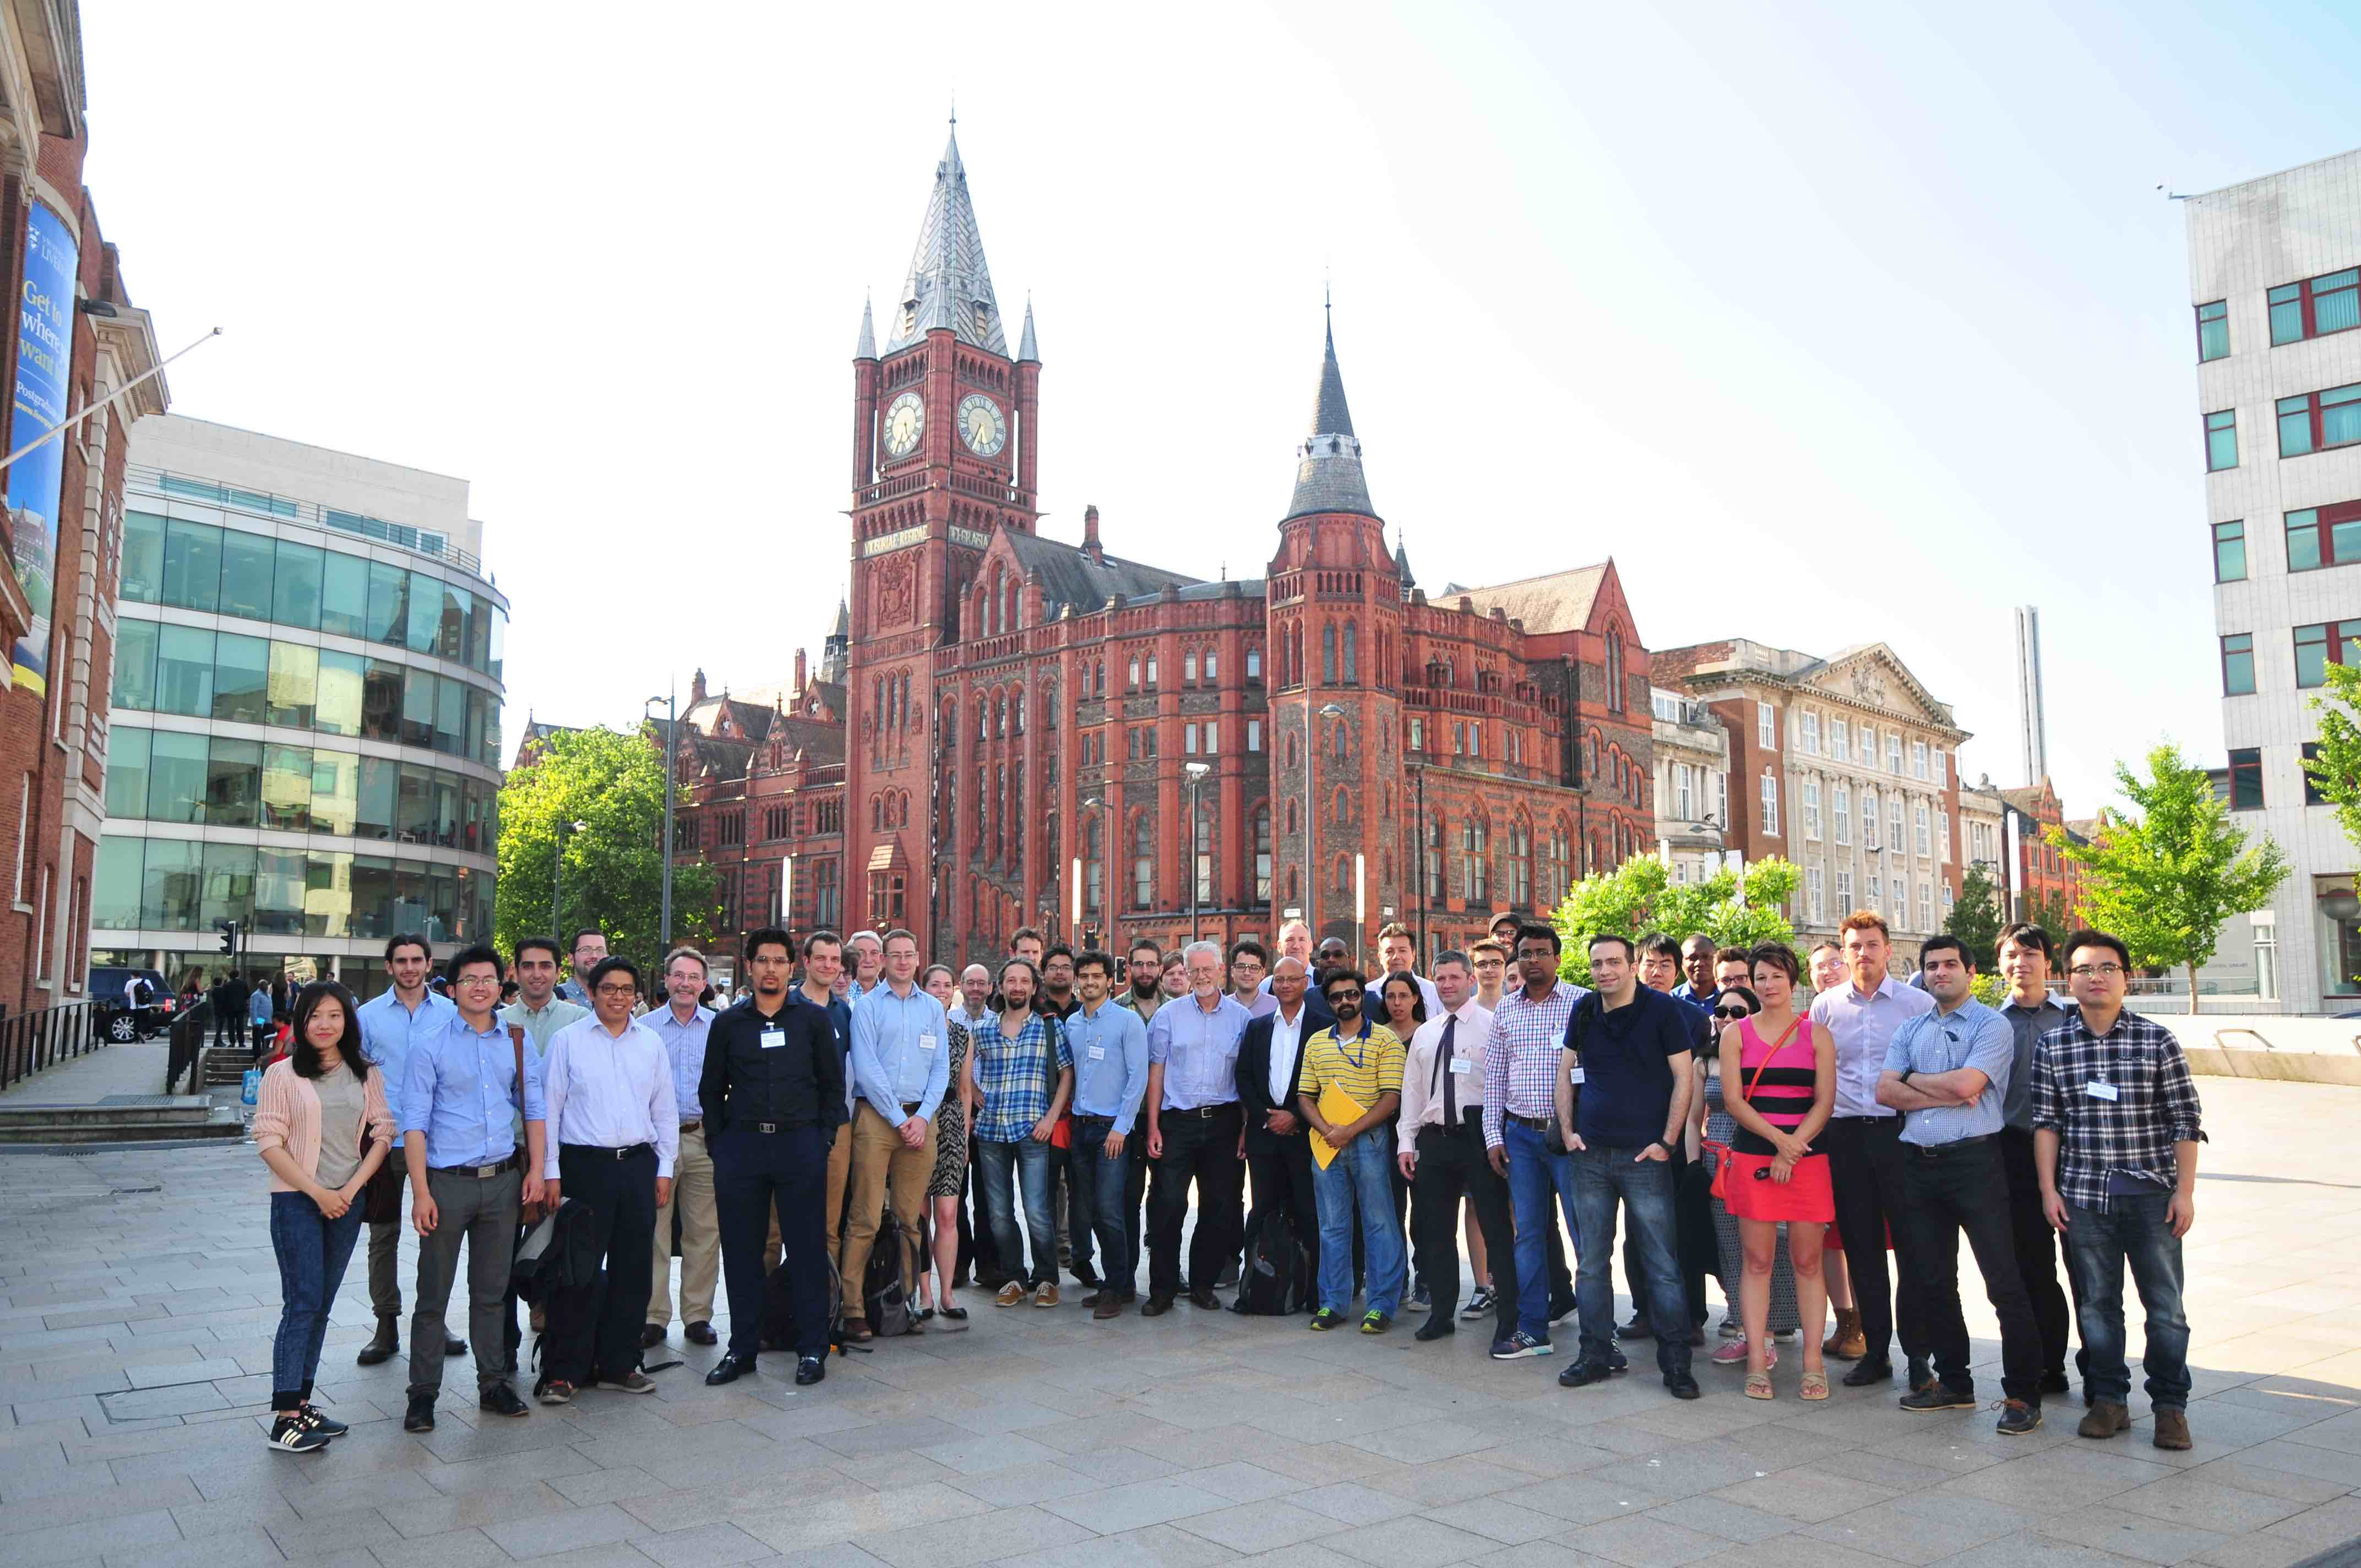
\includegraphics[width=1 \textwidth]{studygroup/picts/groupPicture.JPEG}}}
\end{wrapfigure}
\end{minipage}

\vspace{10pt}

\begin{minipage}{0.31 \linewidth}
 We were also delighted to welcome Colin Armstrong, Head of International Resilience at the Government Office for Science to give a pre-dinner talk on the
\end{minipage}

\begin{minipage}{0.99 \linewidth}
 Tuesday night, which stimulated a lot of interesting discussions  on uncertainty and risk communication during crises such as the outbreak of an epidemic or preventing terrorism. The Study Group served the purpose of addressing industrual challenges (amongst various other purposes) in an open, interactive forum. Sharing methods, exploring the real issues to be tackled and providing (in an intense few days of work) evidence for the necessity for such approaches to be of real benefit to all those who attended.
 
 \href{http://studygroup.riskinstitute.org.uk}{http://studygroup.riskinstitute.org.uk}
\end{minipage}

\vspace{5pt}

\centerline {\rule{1\linewidth}{.25pt}} % Horizontal line

\begin{center}
\href{https://liverpool.ac.uk/risk-and-uncertainty}{
\includegraphics[width=0.03\textwidth]{logos/Risk_cover.png}}\hspace{5pt}
\href{http://liru-cdt.org}{
\includegraphics[width=0.03\textwidth]{logos/icon_tree.png}}
 \hspace{5pt}
\href{https://twitter.com/riskcdt}{
\includegraphics[width=0.03\textwidth]{logos/Twitter_logo.png}}\hspace{5pt}
\href{https://www.flickr.com/photos/125564687@N02/}{
\includegraphics[width=0.03\textwidth]{logos/flickr-logo-png-3.png}}\hspace{5pt}
\end{center}













\cleardoublepage

\thispagestyle{StudyGroup}

\begin{minipage}[t]{.99\linewidth} % Mini page taking up 66% of the actual page
\hypertarget{studyGroup}{\heading{Uncertainty Quantification and Management Study Group with Industry}{1pt}}

%\begin{figure}[H]
%\centering \includegraphics[width=0.9\linewidth]{anas/.jpg}
%\end{figure}
\end{minipage}

Matt Butchers\footnote{Knowledge Transfer Manager, Industrial Mathematics and Sensor Systems at The Knowledge Transfer Network}; Marco De Angelis\footnote{Centre for Doctoral Training in Risk \& Uncertainty Manager, Research Associate, University of Liverpool}, Alejandro Diaz\footnote{Lecturer Applied Mathematics and Statistics, Institute for Risk \& Uncertainty, University of Liverpool}, 


\begin{minipage}[!t]{.25\linewidth}
\begin{mdframed}[style=about,frametitle={}] % Sidebar box


\begin{figure}[H]
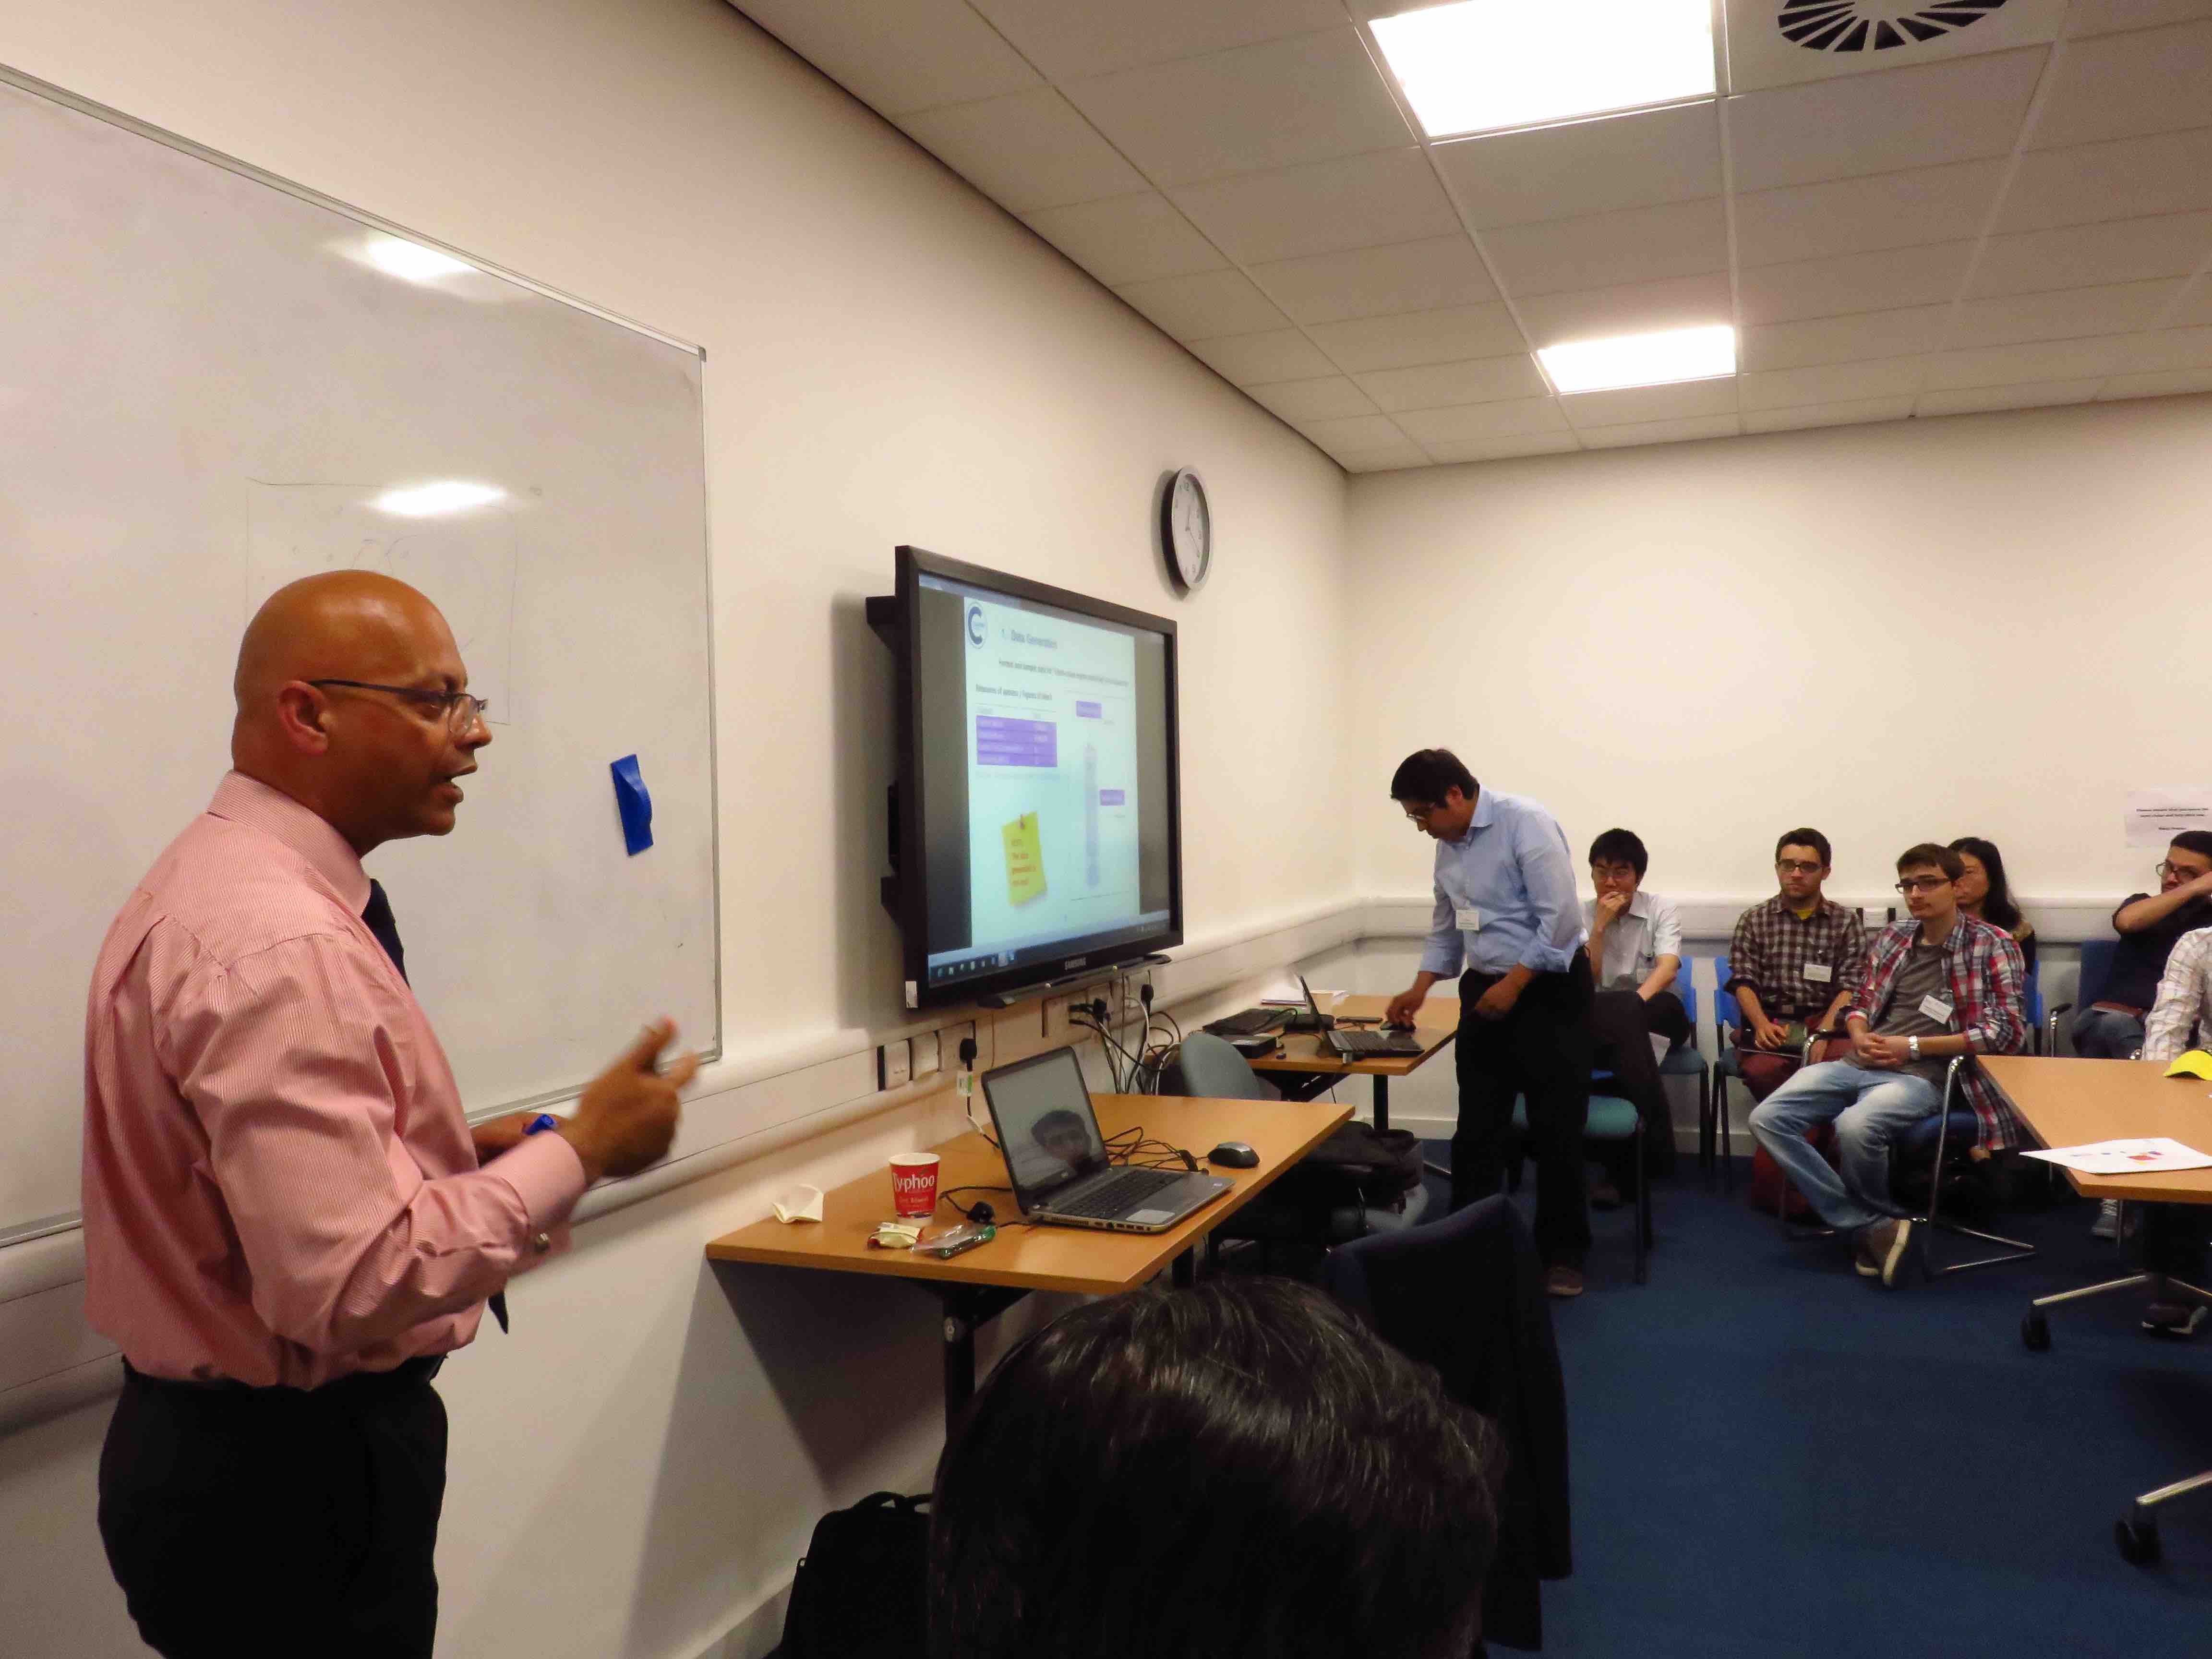
\includegraphics[width=1\linewidth]{studygroup/picts/IMG_1538_lr.jpg}
\end{figure}


``We, the KTN SIG for UQ\&M, wanted to see how the ESGI format would work for UQ\&M. Preparing the industrial case studies beforehand allowed interested academics to participate in the first UQ\&M Study Group, which was held in the Institute for Risk and Uncertainty at the University of Liverpool.
'' - 
{\bf Dr Sanjiv Sharma} - Chair of the UQ\&M SIG

``
I was impressed to see the great synergy between industrialists and academics working side-by-side towards the same goal. The Study Group has given everybody who participated the fantastic opportunity to work closely with top academics in the field of UQ\&M for three days in a row, and to access the very best of practice in this field
'' -
{\bf Dr Marco De Angelis} - Centre for Doctoral Training in Risk \& Uncertainty, University of Liverpool

%Raphael Moura is a Risk/Regulation Engineering Specialist on leave from the Brazilian Regulator for the Oil & Gas Industry (ANP) since October 2013, when he joined the University of Liverpool’s Institute for Risk and Uncertainty as a PhD candidate. 
%
%He has a Master’s degree in Offshore and Ocean Technology (Cranfield University, UK), a Master of Business Administration (FGV-RJ, Brazil), a postgraduate diploma in Offshore Systems Engineering (UFRJ, Brazil) and a Bachelor’s degree in Production Engineering (CEFET-RJ, Brazil). Mr. Moura joined the Brazilian regulator in November 2005, being appointed by the ANP’s Board of Directors as General Manager for Operational Safety in April 2007. He has been dealing with safety inspections, audits and incident investigations at onshore and offshore oil & gas facilities, and played a central role on the establishment of the risk-based safety regulatory framework in Brazil.
\centerline {\rule{1\linewidth}{.25pt}} % Horizontal line


\BackToContents % Link back to the contents of the newsletter

\end{mdframed}\hfill
\end{minipage}
\hspace{0.01\textwidth}
\begin{minipage}[!t]{.75\linewidth}




%\vspace{5pt}
%\includegraphics[width=0.3 \textwidth]{../../issue_1/bruno/nnl-site-logo.png}
%\includegraphics[width=0.2 \textwidth]{../../issue_1/bruno/Page-1.png}

\begin{multicols}{2} % Two-column layout
This Study group aimed to address broad industrial challenges in UQ\&M by tackling three case studies supplied by \textbf{Jaguar Land Rover}, \textbf{Airbus}, and \textbf{Zenotech}. 

The purpose of the Study group was four-fold:
\begin{itemize}
    \item To help companies with established UQ programmes refine their approaches,
    \vspace{5pt}
    \item To help companies new to the field understand the benefit that UQ\&M could have on their operations,
    \vspace{5pt}
    \item To expose UK researchers to the kind of challenges UK industries wish to apply UQ\&M to, and
    \vspace{5pt}
    \item To enable a cross-fertilisation of ideas between disciplines (data scientists, statisticians, numerical analysts etc.).
\end{itemize}

\vspace{5pt}
{\bf The Problems and Approaches}

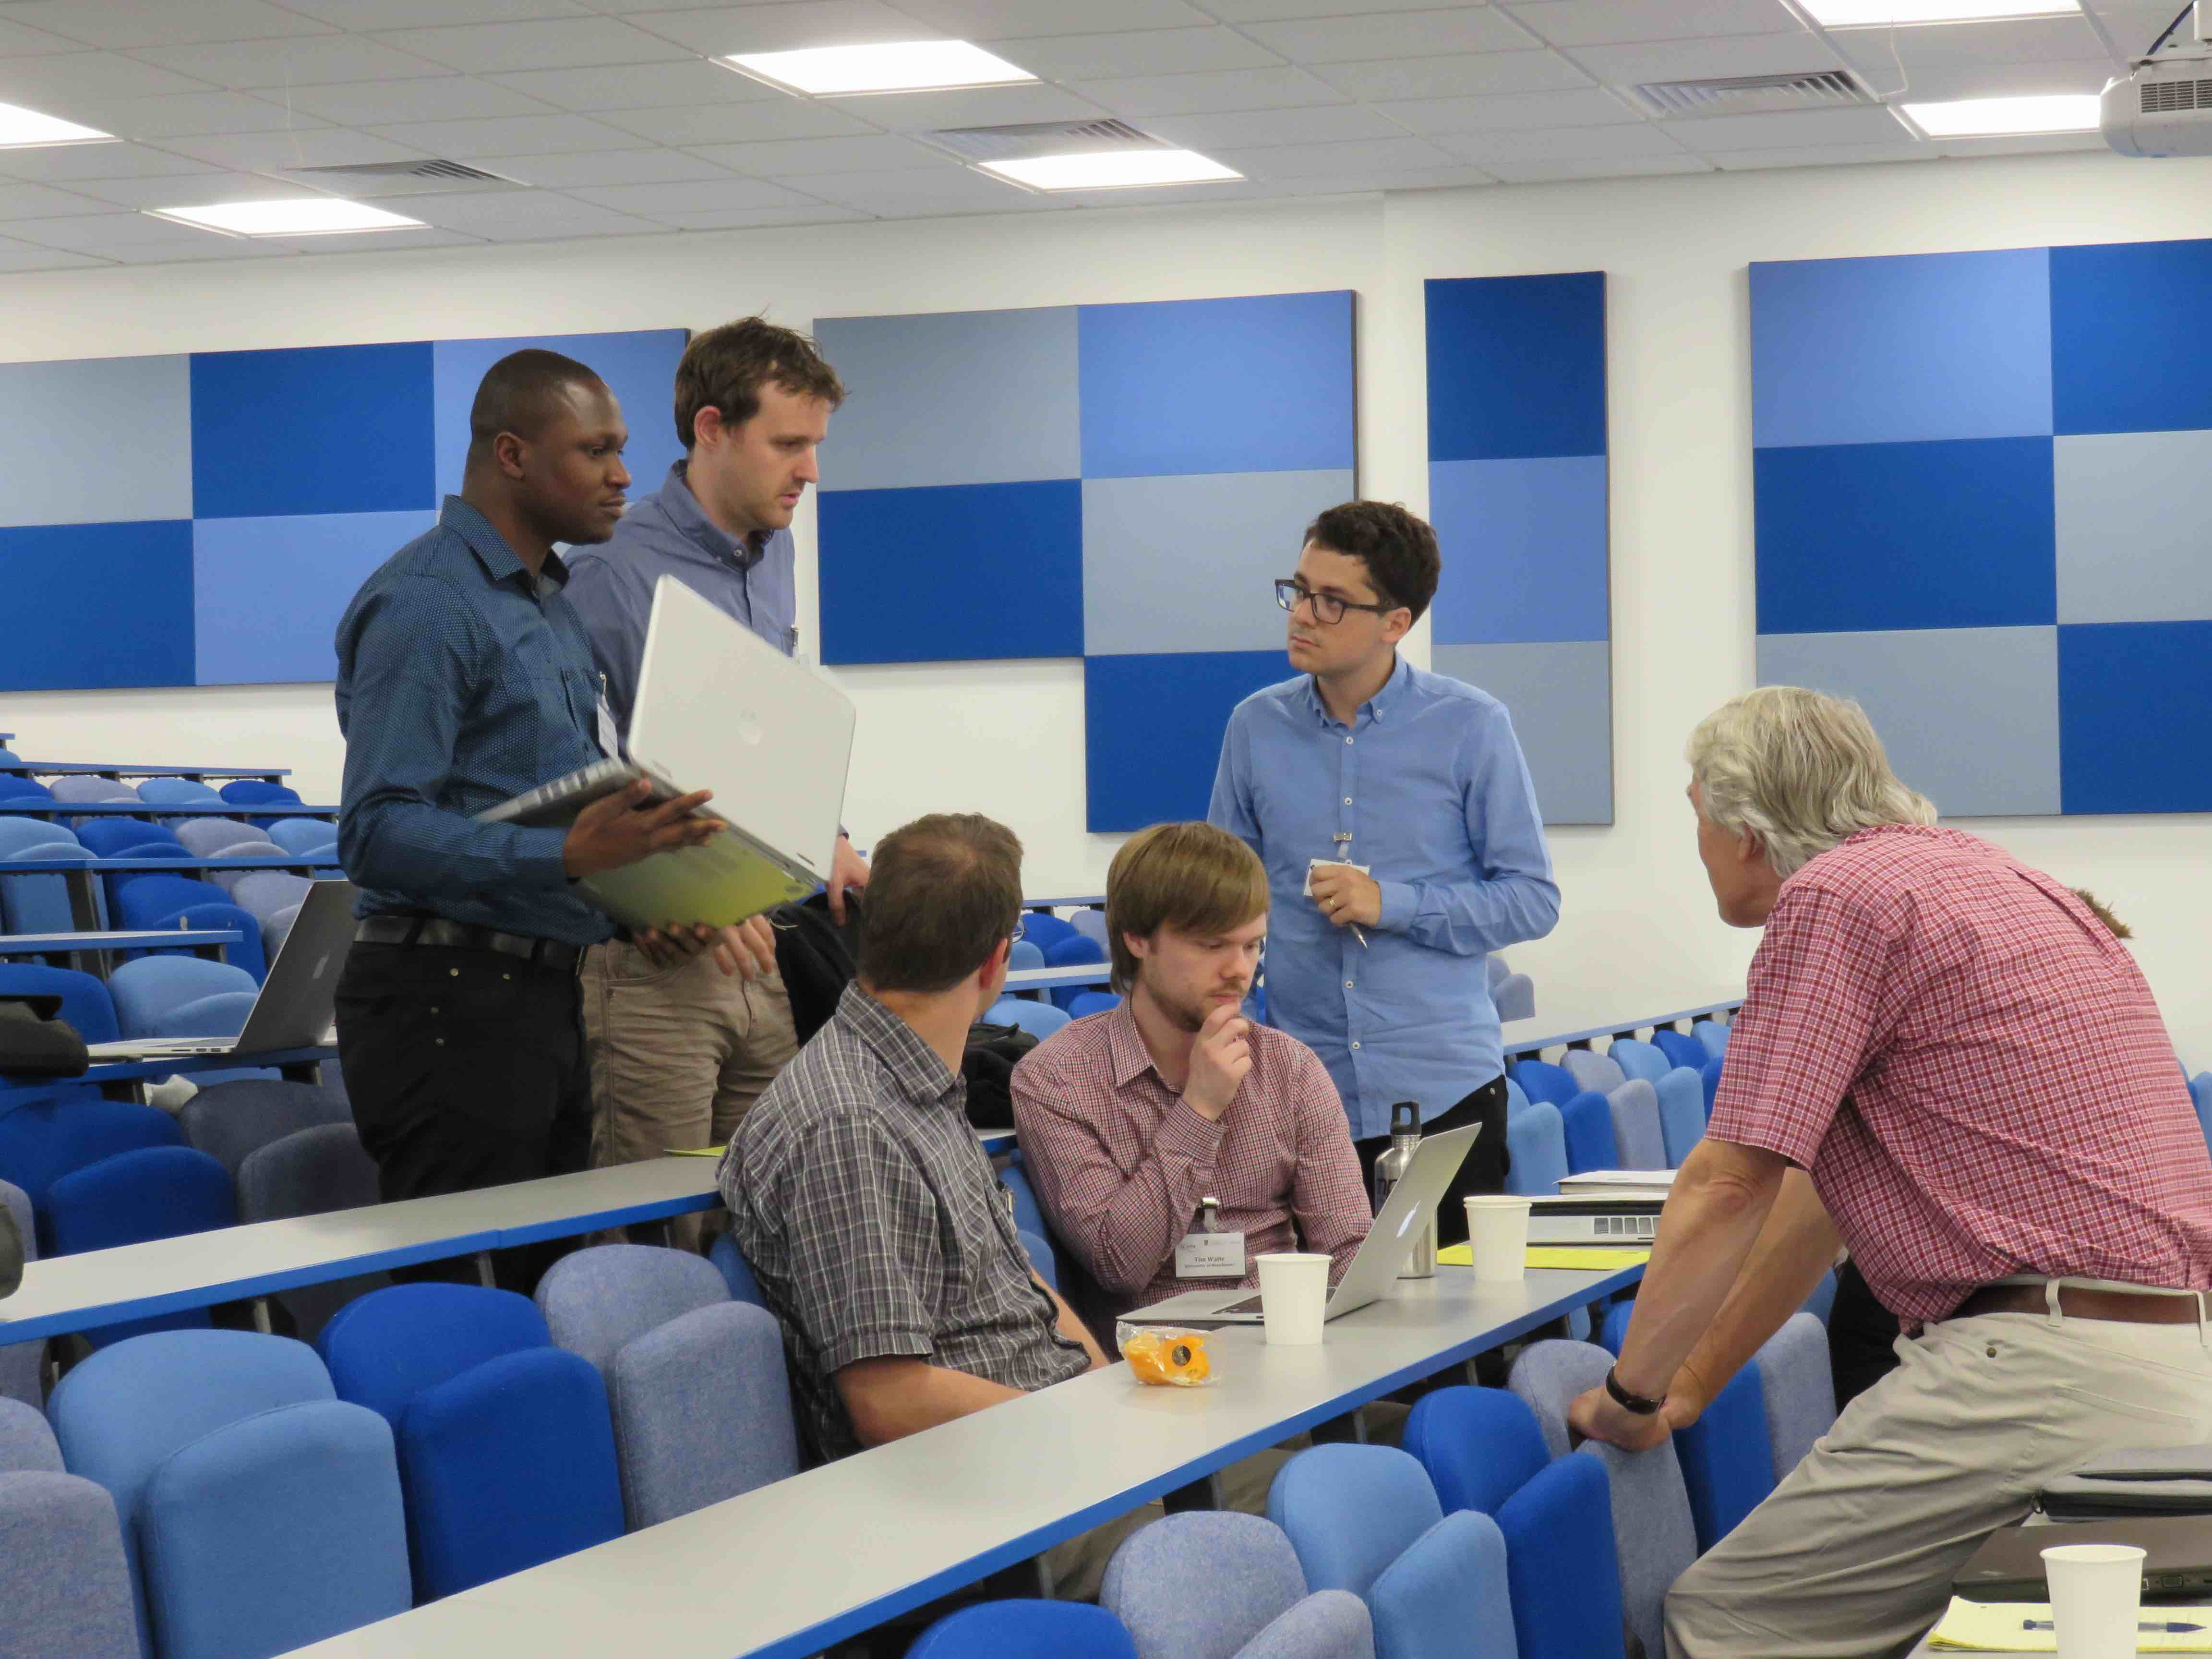
\includegraphics[width=0.5 \textwidth]{studygroup/picts/IMG_1580_lr.jpg}

{\bf Jaguar Land Rover} (JLR) came to the Study Group looking to address how to optimise the ride performance of a vehicle when mass property variations are taken into account, and how UQ\&M could be used to minimise the number of components required to achieve the desired ride performance metrics. Jacqui Morison and Peter Newbury (JLR) outlined their challenge on the Monday morning along with the other industries; all of whom attracted a huge amount of questions and comments. A self-organised group then explored various tasks for JLR including Gaussian process modeling and optimisation (maximising the probability of meeting design specifications), visualisation, robust design and tailored model-based design of experiments.

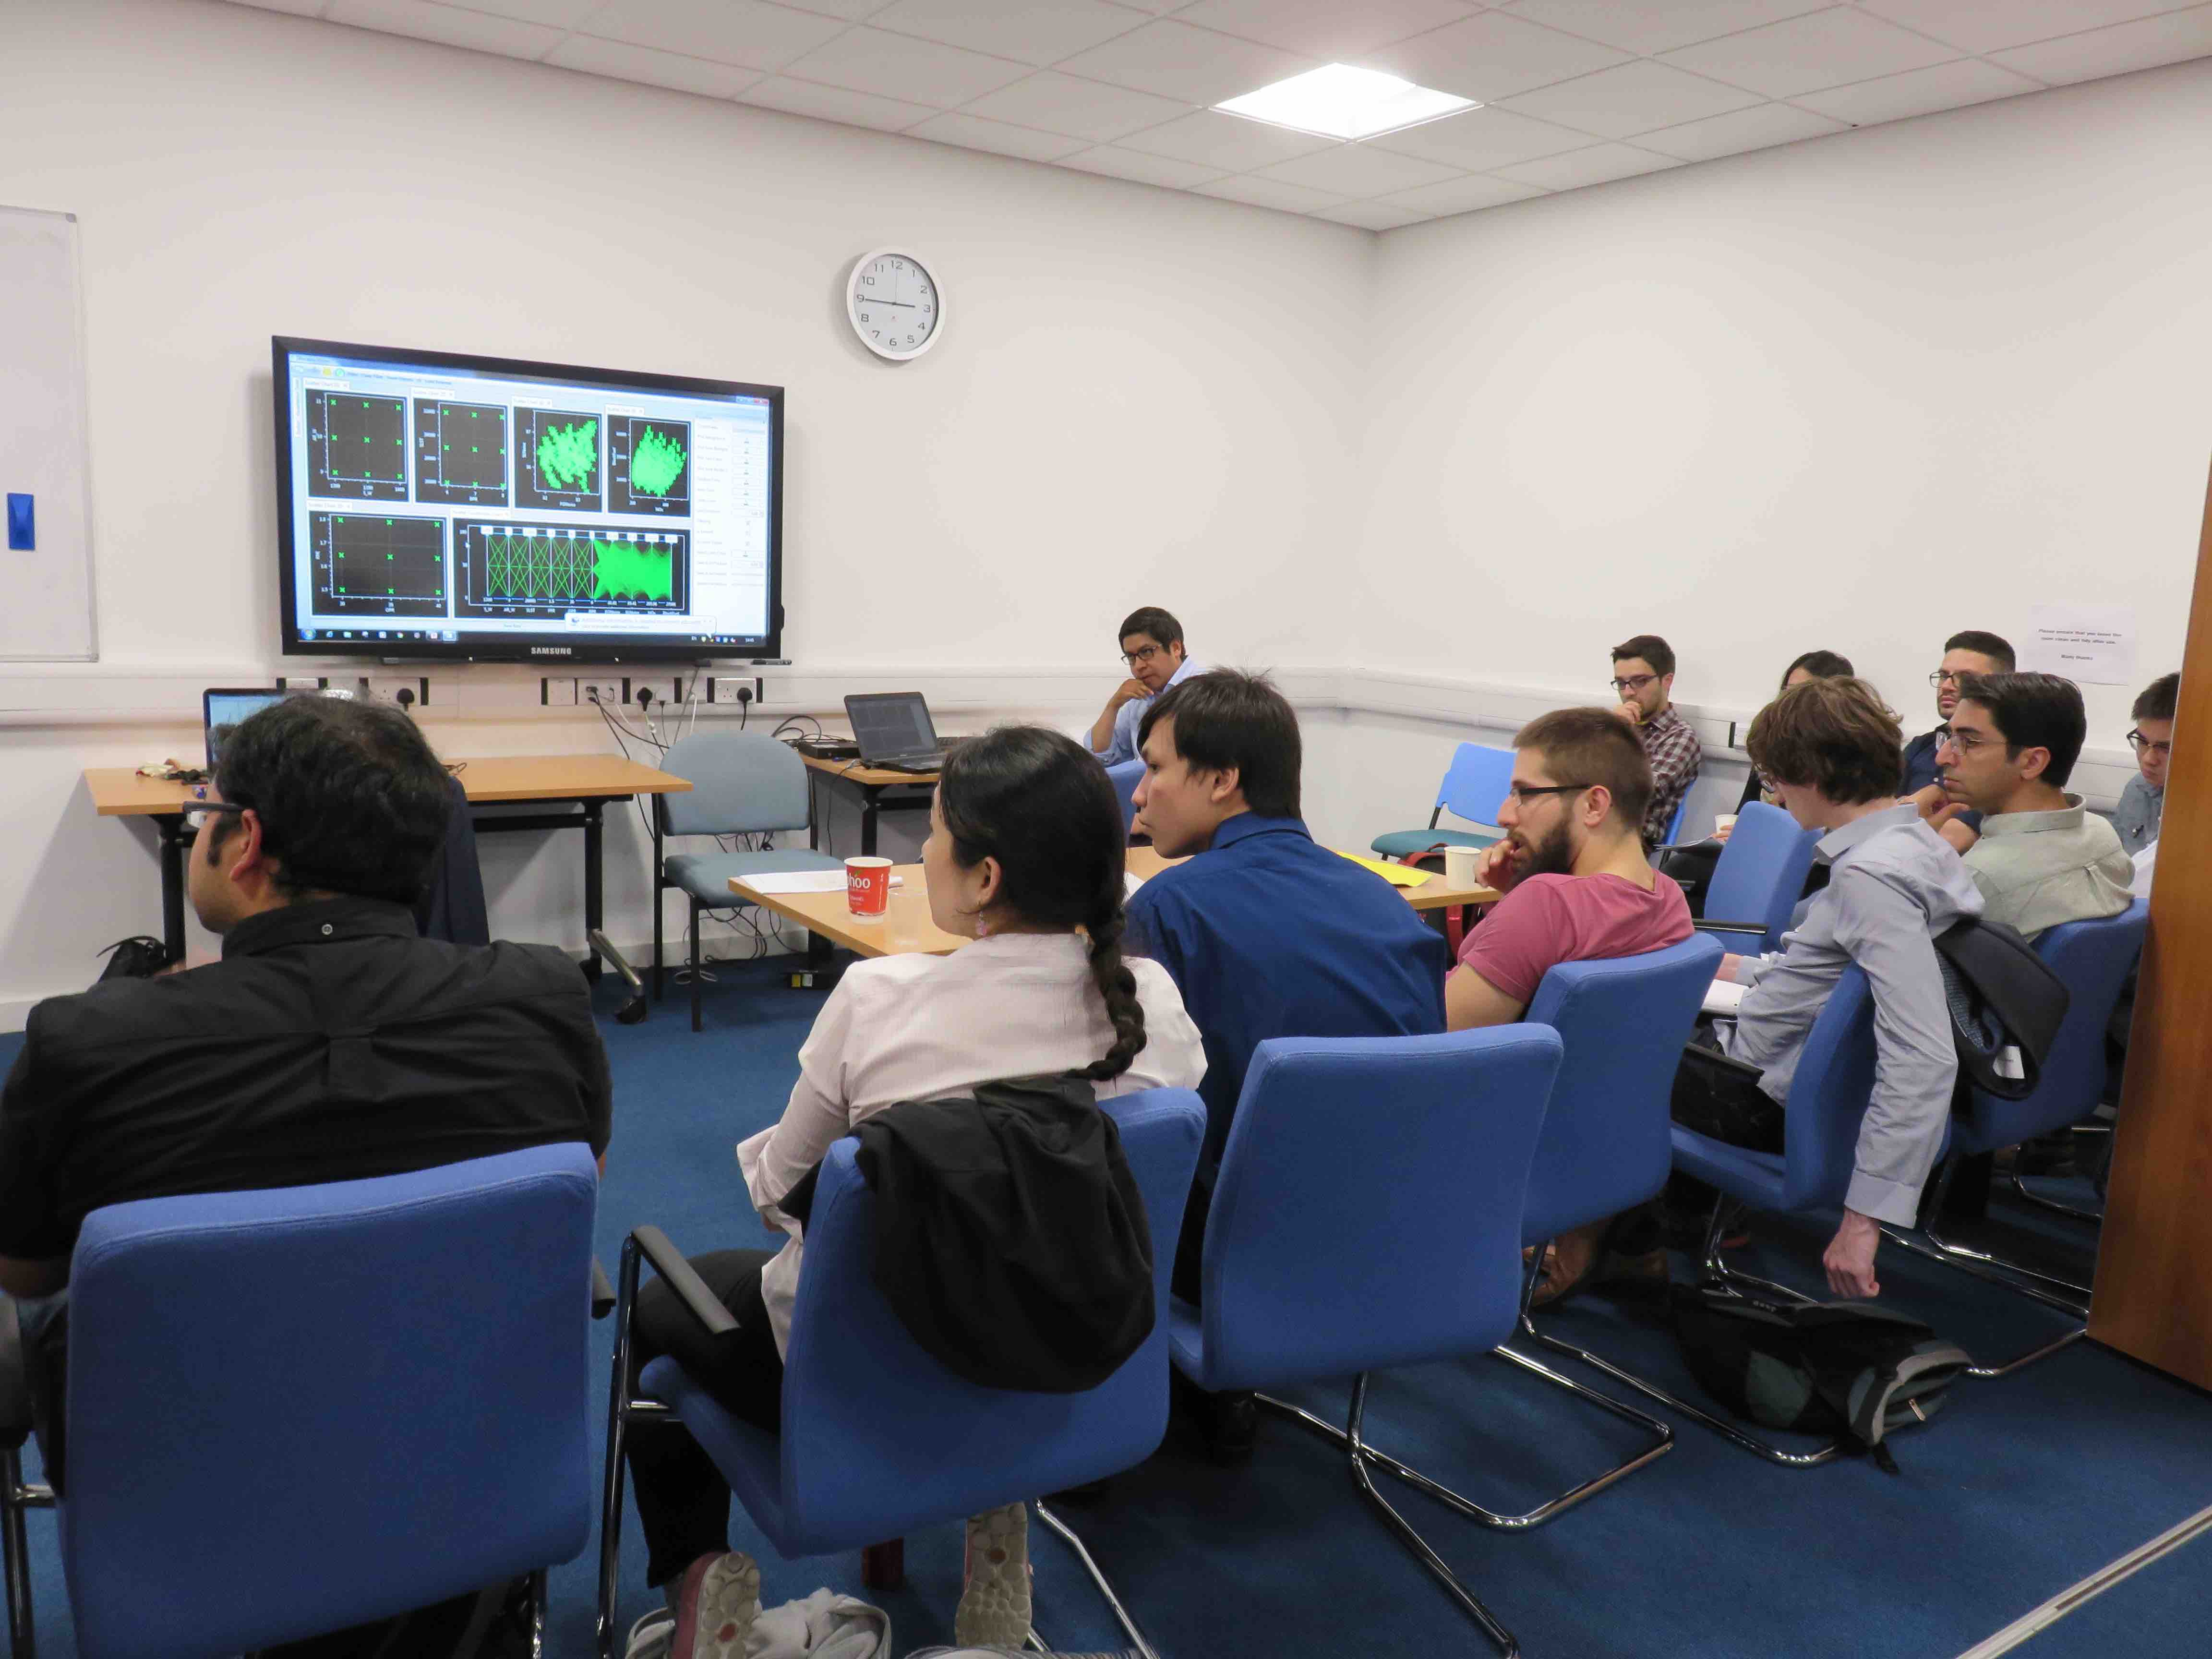
\includegraphics[width=0.5 \textwidth]{studygroup/picts/IMG_1592_lr.jpg}

Sanjiv Sharma from {\bf Airbus} presented his challenge - Climb-cruise Engine Matching. Sanjiv sought UQ\&M techniques that could better narrow a set of possible aircraft design configurations when uncertainty in introduced. This group explored ideas around history matching (determining input values which relate to a predetermined output range), finding key parameters of interest through global sensitivity analysis, and finding dependencies between inputs and outputs.




%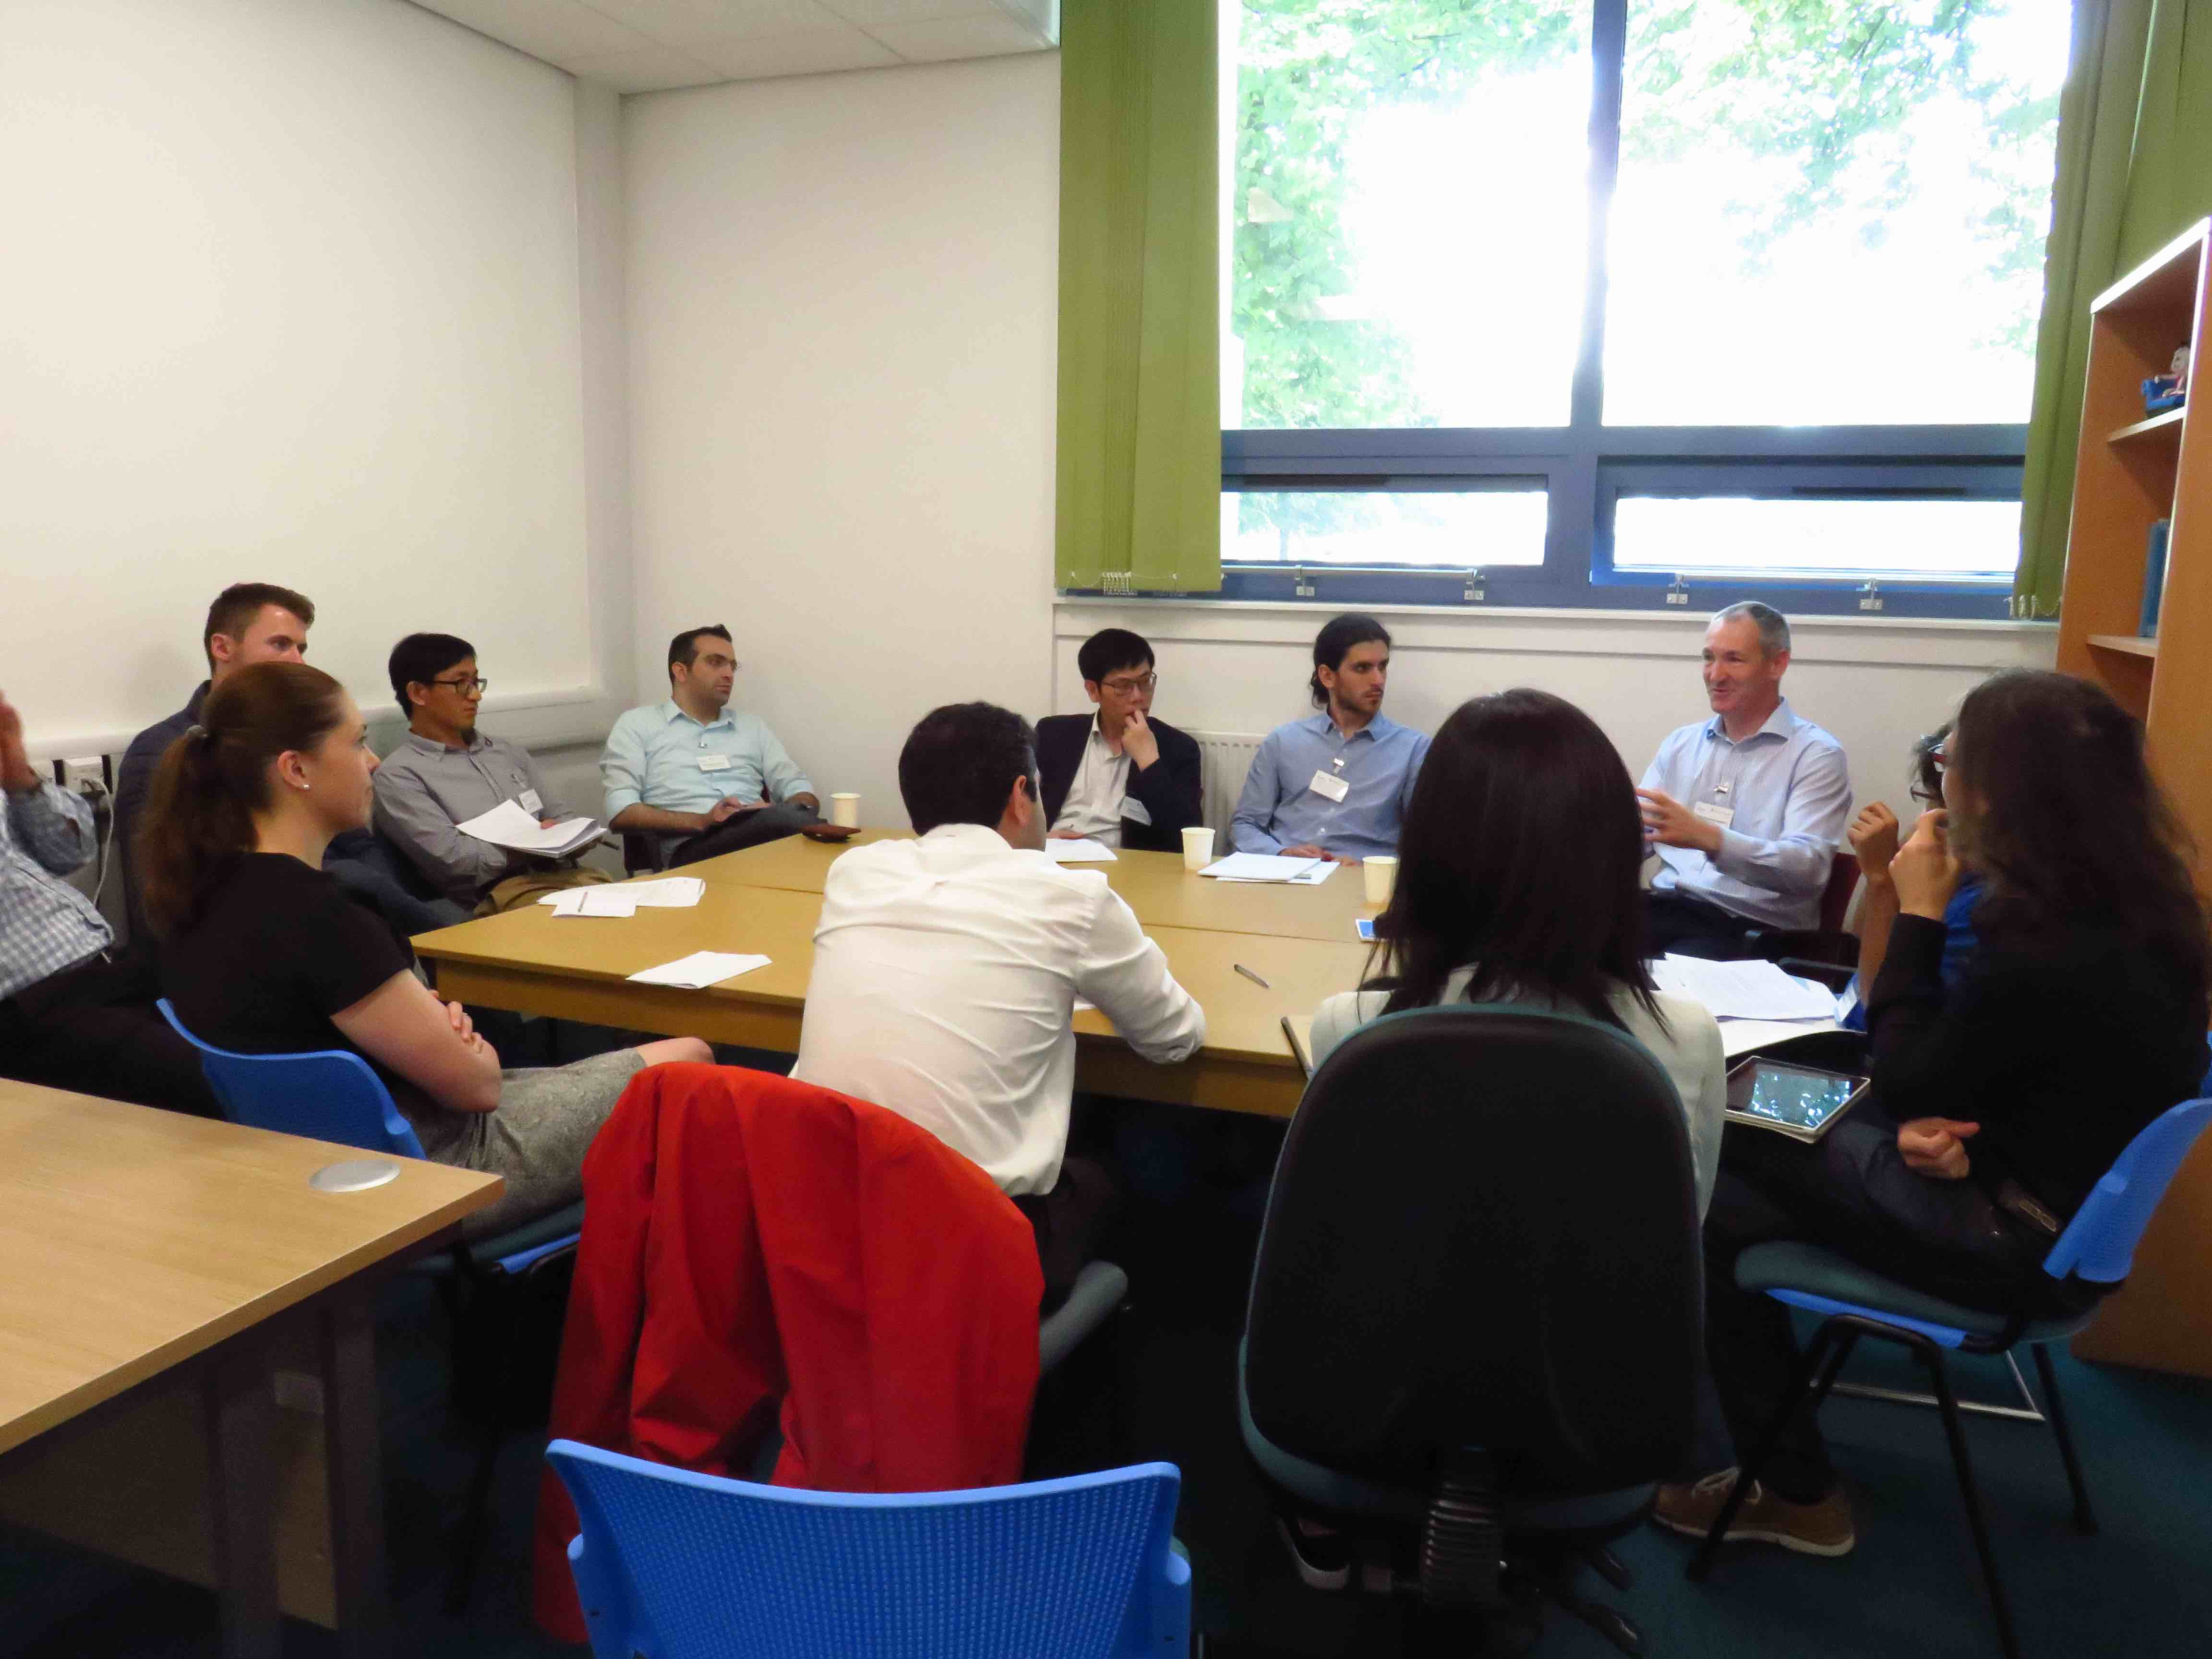
\includegraphics[width=0.5 \textwidth]{studygroup/picts/IMG_1536_lr.jpg}

%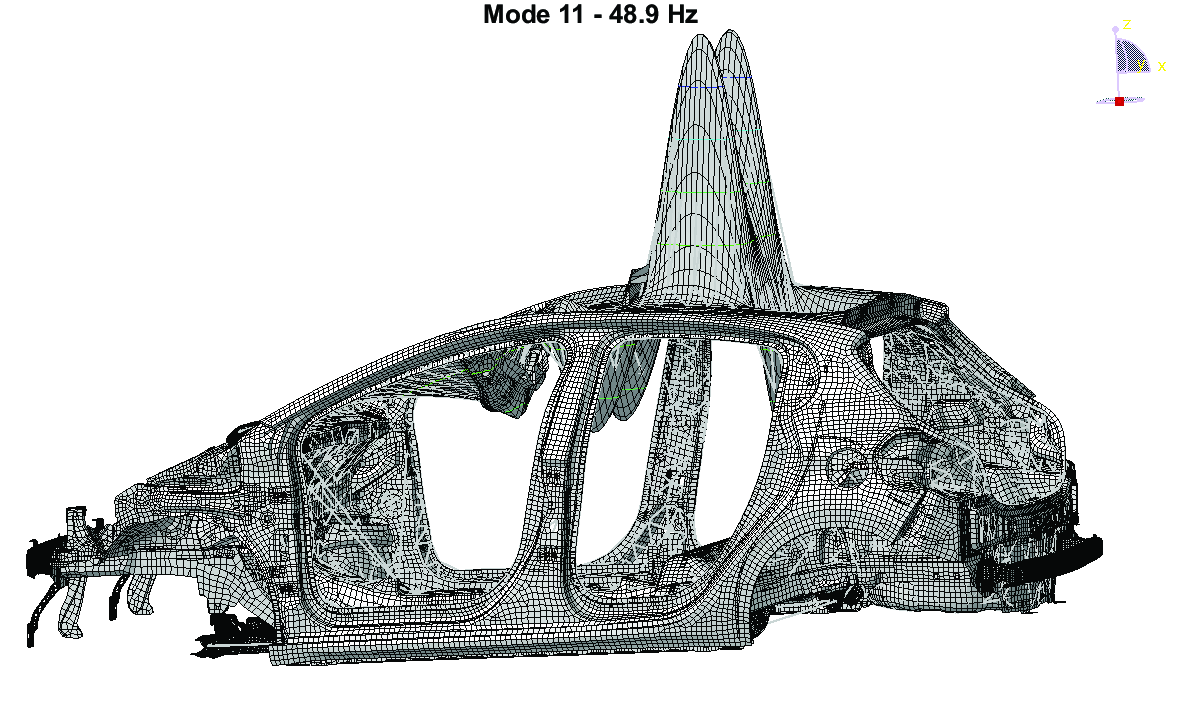
\includegraphics[width=0.5 \textwidth]{anas/fig1.png}
%{\scriptsize BIW automobile - Example of global mode belonging to the low-dimension Reduced-Order Basis}\\
%\begin{wrapfigure}[16]{r}[0pt]{0.8 \textwidth}
%\centering
%\includegraphics[width=0.8 \textwidth]{../../issue_1/bruno/figure.jpg}
%\vspace{-40pt}
%\caption{Future plan for Germany's phase out}
%\end{wrapfigure}

%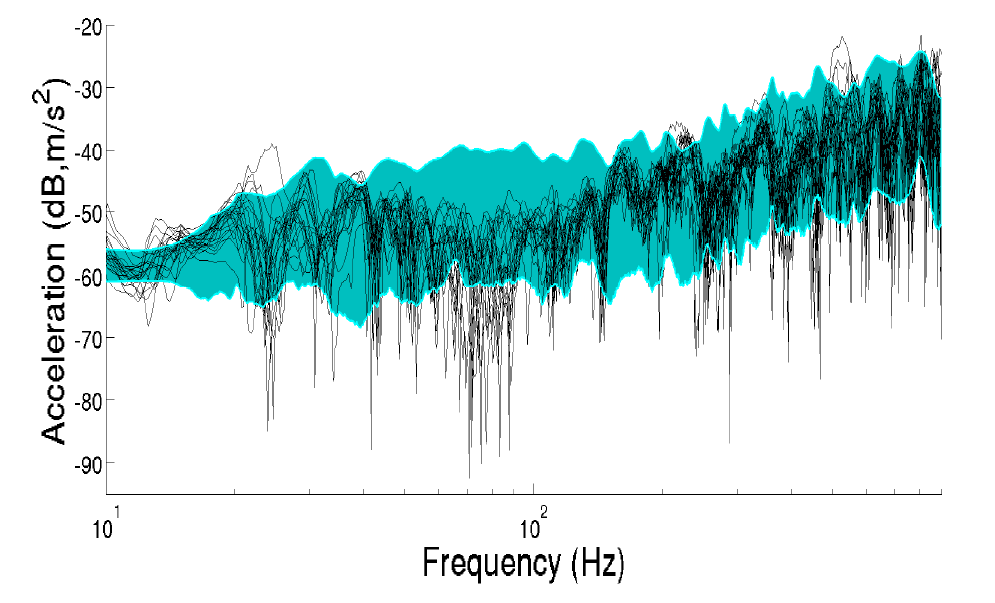
\includegraphics[width=0.5 \textwidth]{anas/fig2.png}
%{\scriptsize Experimental FRF measurements (black lines) and random FRF using the SROM (colored region)}\\

 
%\begin{wrapfigure}[5]{r}[0pt]{0.2 \textwidth}
%\vspace{-10pt}
%
\includegraphics[width=0.18 \textwidth]{anas/logoLR.jpg}
%\end{wrapfigure}


%\begin{wrapfigure}[3]{r}[0pt]{0.3 \textwidth}
%\centering
%
%\end{wrapfigure}

\end{multicols}
\end{minipage}










\cleardoublepage

\thispagestyle{StudyGroup}
\begin{minipage}[t]{.99\linewidth}
\vspace{0.1cm}
\end{minipage}

\begin{minipage}[t]{.99\linewidth} % Mini page taking up 66% of the actual page
\begin{multicols}{2}

David Standingford, Director of {\bf Zenotech} - an SME in the HPC and CFD space - posed the challenge of increasing certainty in offshore energy installations by checking the validity of CFD simulations. It was commented that a fraction reduction in damage caused by unpredicted wake effects could result in substantial cost savings for the energy industry. The Zenotech team worked to calibrate the CFD model with experimental data, create metamodels for the objective function, and use Bayesian optimisation given the expensive computer execution.

\vspace{10pt}
\begin{center}
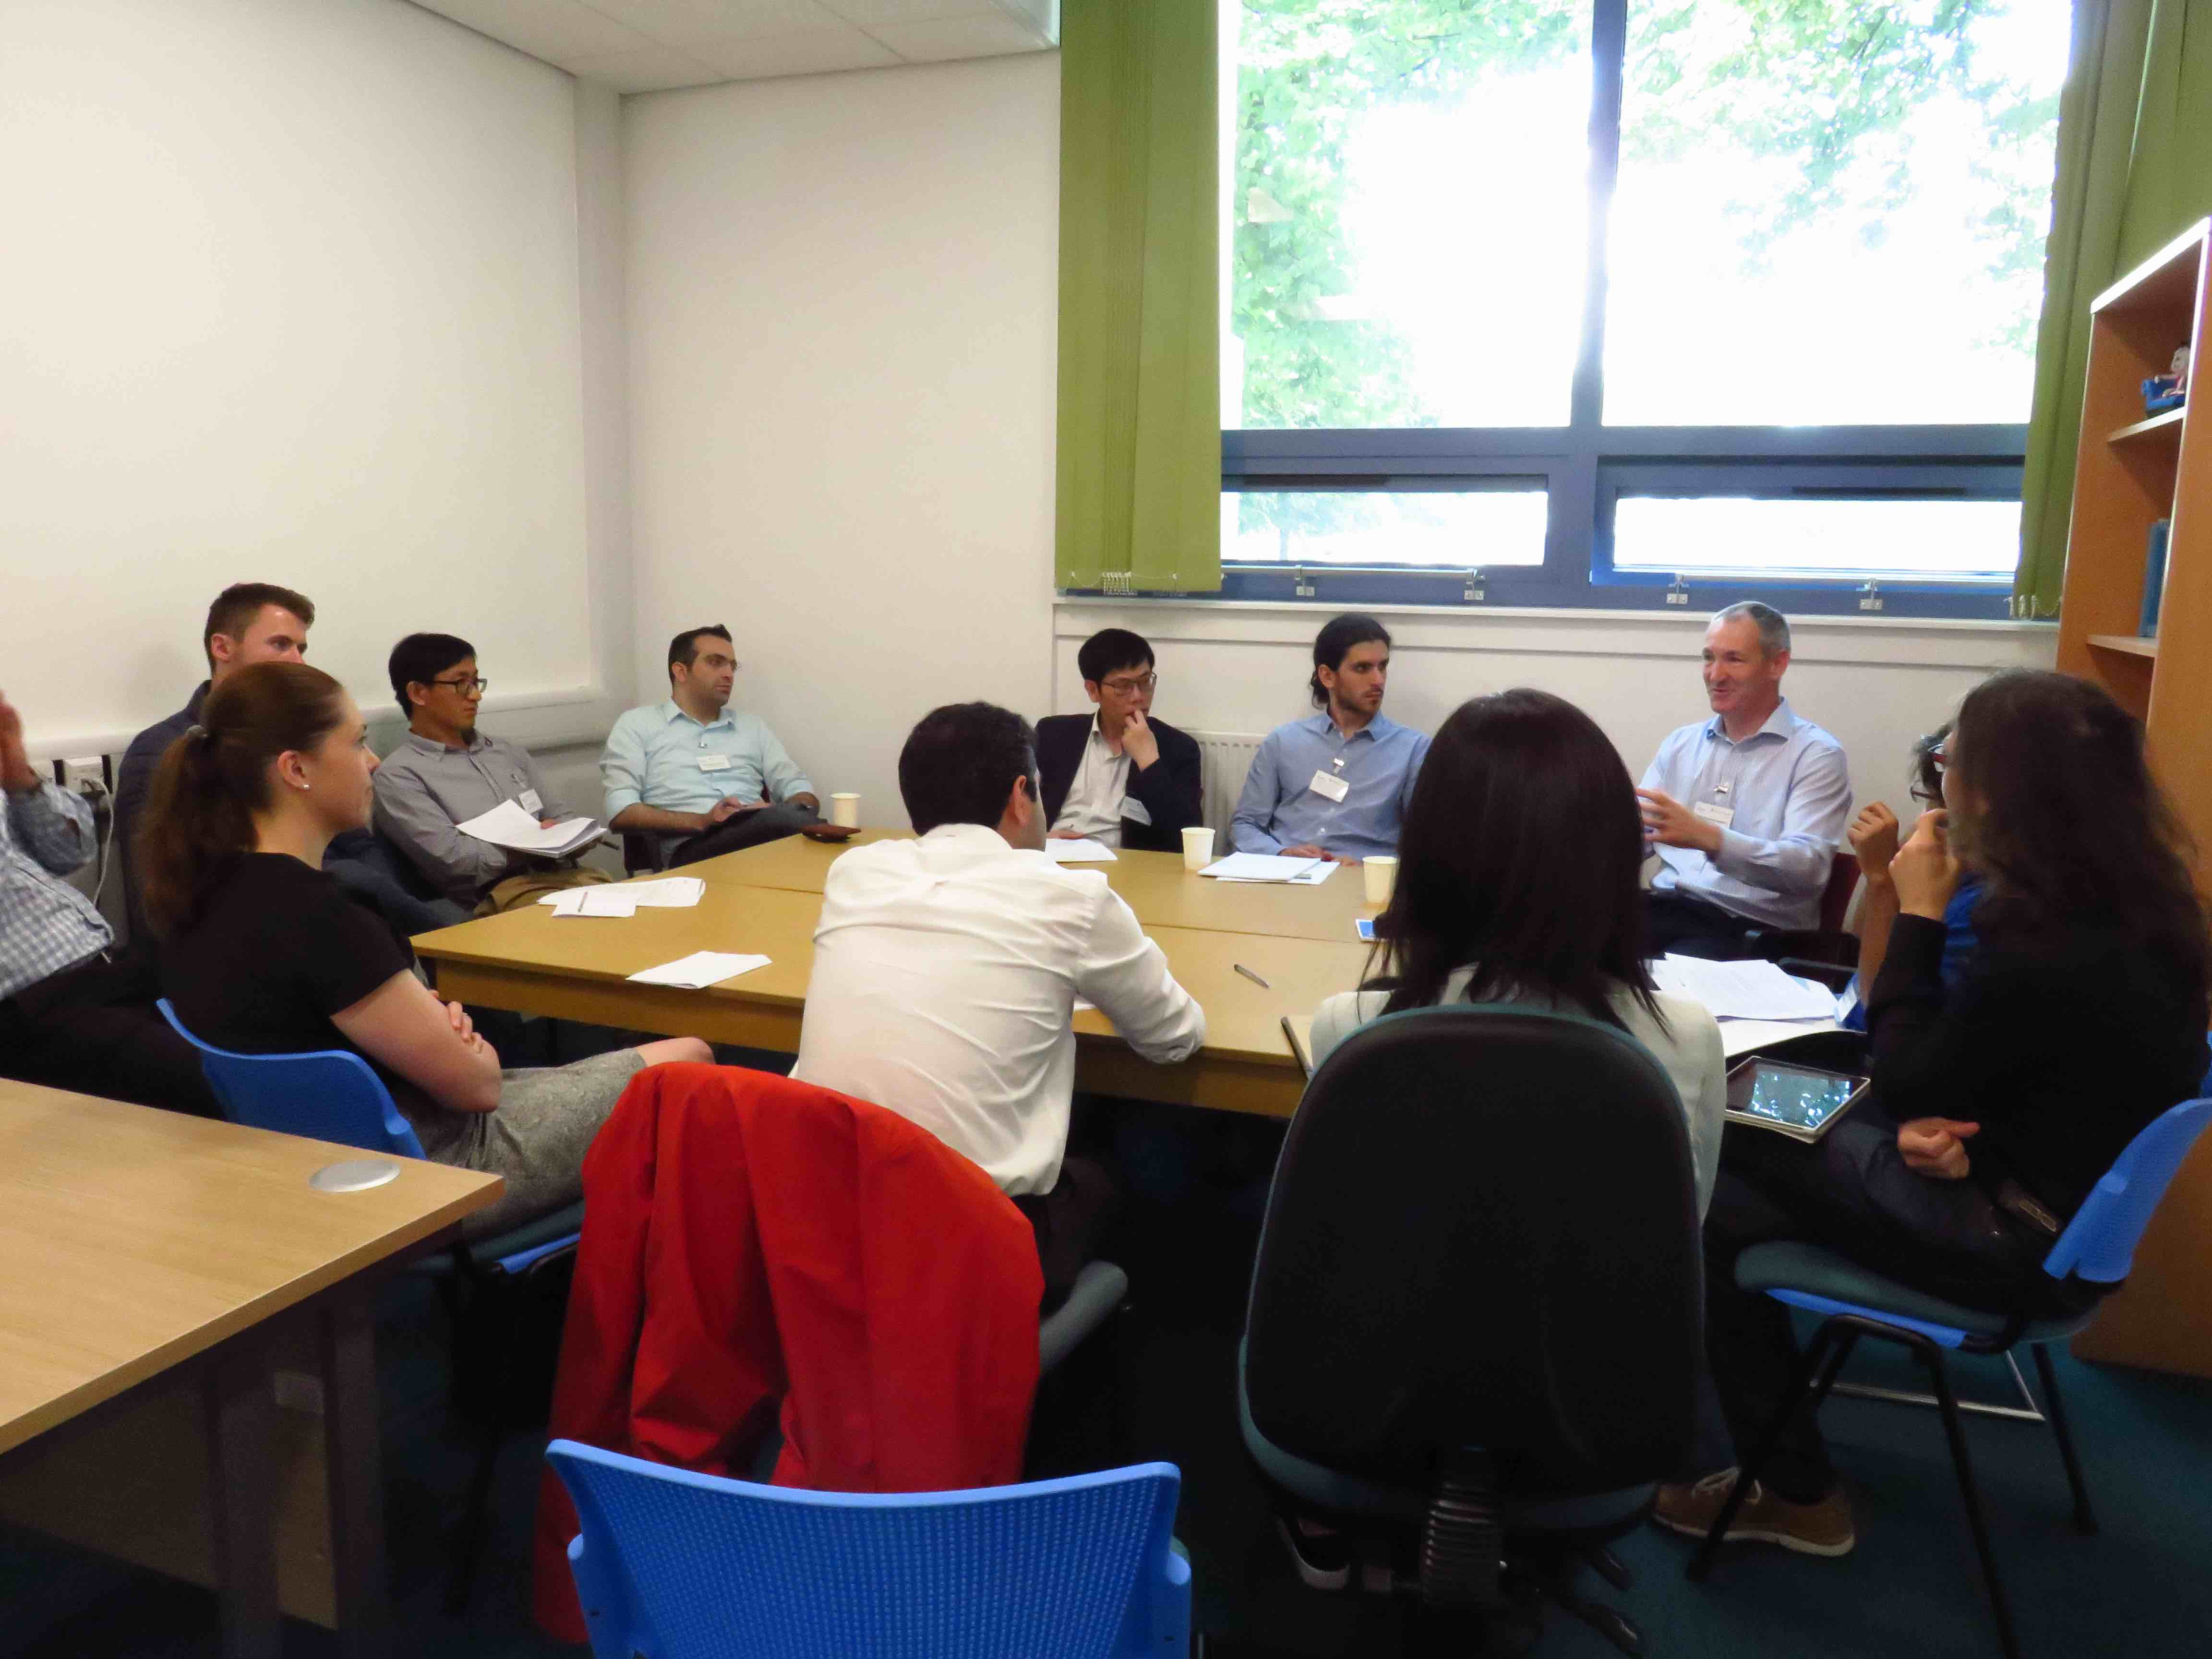
\includegraphics[width=0.46 \textwidth]{studygroup/picts/IMG_1536_lr.jpg}
\end{center}

\vspace{10pt}
\begin{mdframed}[style=about,frametitle={}, leftmargin=20pt, rightmargin=20pt] % Sidebar box
\vspace{5pt}
    `` At this inaugural event, three industrial case studies were presented during the first morning. This allowed researchers to assess where they wished to contribute, initially. Of course, they were free to move from one industrial case study to another; we maintained continuity by assigning a leader for each group who would stay with the case study and report on the findings. The buzz of conversations that took place to refine the problem statements, propose solutions, and test ideas was exciting - equally so for the industrialists, both as observers and as participants, because we were treated as an integral part of the Study Group. Through these conversations we jointly developed a better understanding of the problem whereby the researchers could seek appropriate solutions. A stimulating aspect of the self-organised researchers was that they were from different universities and different disciplines; yet by working together perhaps they have created opportunities for new collaboration beyond the Study Group. '' 

- {\bf Dr Sanjiv Sharma} - Chair of the UQ\&M SIG

\BackToContents % Link back to the contents of the newsletter
\end{mdframed}\hfill

\vspace{25pt}
{\bf Why UQ\&M in Manufacturing?}
Manufacturing contributes over £6.7 tr to the global economy and the UK is a major contributor. In terms of manufacturing Gross Value Added (GVA) the UK is in the world's top 10, generating 10\% of UK GVA. UK manufacturing directly employs 2.5 million people, generates half of UK exports and accounts for three quarters of business R\&D conducted in the UK.

Virtual design through modeling and simulation is extremely attractive for high value manufacturing. Virtual design can:
\begin{enumerate}
    \item Significantly speed up the development cycle (i.e. reduction of time from an idea to its implementation, that is very important for complex platforms and products), and
    \item Substitute with simulations some real-life tests necessary in many cases for approval of new materials, designs, platforms etc.
\end{enumerate}
When bringing a new product from conception into production, success rests on the careful management and control of risk in the face of many interacting uncertainties. Historically, chief engineers and project managers have estimated and managed risk using mostly human judgment founded upon years of experience and heritage. As the timescale from concept to commercialisation is eroding, there is decreasing time to build 'experience and heritage', and turnover of personnel and the cost of personnel time both mean that it is not practical to pass on all that 'experience and heritage' to one's successors.

In an era of virtual design, there is an opportunity to handle uncertainty in a systematic way, and create designs robust against these uncertainties. Today's fiercely competitive market and increasingly stringent regulatory environment is such that there is very little margin for error. Failure to understand and manage risks can result in severe financial penalties and even damage to reputation.

%{\bf Current State of Industrial Adoption of UQ\&M}
%Uptake of formal UQ\&M methods in HVM is a mixed bag. A recent project exploring the use of modeling and simulation in HVM performed by NAFEMS, Innovate UK, GE Power and KTN found no best practice was observed across the wide HVM sectors. Few formal programmes of activity were present, and where they were they were generally limited to sensitivity analysis.

%Reasons for the lack of uptake vary from sector to sector; for example those in the process industries stated that data uncertainties were to difficult to capture reliably. Cost, knowledge of decision makers, interpretation, and time all scored highly across HVM sectors

%The Study Group served the purpose of addressing these challenges (amongst various other purposes) in an open, interactive forum. Sharing methods, exploring the real issues to be tackled and providing (in an intense few days of work) evidence for the necessity for such approaches to be of real benefit to all those who attended.

{\bf What next?}
Reports for each case will be written and distributed by the organisers. Additionally, we wish to create a report which is of general interest and use to the wider manufacturing community.

Finally, given the very positive response in outputs and enjoyment of the process we would wish to explore the possibility of running such activities again. If you wish to know more about the 2016 Study Group for UQ\&M, or would like to take part in future activities, please do not hesitate to contact us.


\end{multicols}
\end{minipage}











%Members of the UK Uncertainty Quantification & Management (UQ&M) research community gathered in Liverpool this Summer for a joint Study Group run by the UQ&M SIG and the Institute for Risk and Uncertainty. This Study group aimed to address broad industrial challenges in UQ&M by tackling three use cases supplied by Jaguar Land Rover, Airbus, and Zenotech.

%The Study Group

%The Study Group focused around three industrial problems. Jaguar Land Rover, Zenotech and Airbus came with challenges and members of the UK research base were invited to attend for three days to work on them. We were also delighted to welcome Colin Armstrong, Head of International Resilienace at the Government Office for Science to give a pre-dinner talk on the Tuesday night, which stimulated a lot of interesting discussions on uncertainty and risk communication during crises such as the outbreak of an epidemic or preventing terrorism.

%The purpose of the Study group was four-fold:

%1. To help companies with established UQ programmes refine their approaches,
%2. To help companies new to the field understand the benefit that UQ&M could have on their operations,
%3. To expose UK researchers to the kind of challenges UK industries wish to apply UQ&M to, and
%4. To enable a cross-fertilisation of ideas between disciplines (data scientists, statisticians, numerical analysts etc.)
%“I was impressed to see the great synergy between industrialists and academics working side-by-side towards the same goal. The Study Group has given everybody who participated the fantastic opportunity to work closely with top academics in the field of UQ&M for three days in a row, and to access the very best of practice in this field.”

%- Marco de Angelis, CDT Manager, Institute for Risk and Uncertainty

%The Problems and Approaches

%Jaguar Land Rover (JLR) came to the Study Group looking to address how to optimise the ride performance of a vehicle when mass property variations are taken into account, and how UQ&M could be used to minimise the number of components required to achieve the desired ride performance metrics. Jacqui Morison and Peter Newbury (JLR) outlined the challenge on the Monday morning along with the other industries; all of whom attracted a huge amount of questions and comments. A self-organised group then explored various tasks for JLR including Gaussian process modelling and optimisation (maximising the probability of meeting design specifications), visualisation, robust design and tailored model-based design of experiments.

%Sanjiv Sharma from Airbus UK presented his challenge – Climb-cruise Engine Matching. Sanjiv sought UQ&M techniques that could better narrow a set of possible aircraft design configurations when uncertainty is introduced. This group explored ideas around history matching (determining input values which relate to a predetermined output range), finding key parameters of interest through global sensitivity analysis, and finding dependencies between inputs and outputs.

%David Standingford, Director of Zenotech – an SME in the HPC and CFD space – posed the challenge of increasing certainty in offshore energy installations by checking the validity of CFD simulations. It was commented that a fraction reduction in damage caused by unpredicted wake effects could result in substantial cost savings for the energy industry. The Zenotech team work to clibrate the CFD model with experimental data, create metamodels for the objective function, and use Bayesian optimisation given the expensive computer execution.


%Why UQ&M in Manufacturing?

%Manufacturing contributes over £6.7 tr to the global economy and the UK is a major contributor. In terms of manufacturing Gross Value Added (GVA) the UK is in the world’s to 10, generating 10 % of UK GVA. UK manufacturing directly employs 2.5 million people, generates half of UK exports and accounts for three quarters of business R&D conducted in the UK [1]

%Virtual design through modelling and simulation is extremely attractive for high value manufacturing. Virtual design can:

%1. Significantly speed up the development cycle (i.e. reduction of time from an idea to its implementation, that is very important for complex platforms and products), and
%2. Substitute with simulations some real-life tests necessary in many cases for approval of new materials, designs, platforms etc. [2]
%When bringing a new product from conception into production, success rests on the careful management and control of risk in the face of many interacting uncertainties. Historically, chief engineers and project managers have estimated and managed risk using mostly human judgment founded upon years of experience and heritage. As the timescale from concept to commercialisation is eroding, there is decreasing time to build ‘experience and heritage’, and turnover of personnel and the cost of personnel time both mean that it is not practical to pass on all that ‘experience and heritage’ to one’s successors.

%In an era of virtual design, there is an opportunity to handle uncertainty in a systematic way, and create designs robust against these uncertainties. Today’s fiercely competitive market and increasingly stringent regulatory environment is such that there is very little margin for error. Failure to understand and manage risks can result in severe financial penalties and even damage to reputation. [3]

%Current State of Industrial Adoption of UQ&M

%Uptake of formal UQ&M methods in HVM is a mixed bag. A recent project exploring the use of modeling and simulation in HVM performed by NAFEMS, Innovate UK, GE Power and KTN found no best practice was observed across the wide HVM sectors. Few formal programmes of activity were present, and where they were they were generally limited to sensitivity analysis.

%Reasons for the lack of uptake vary from sector to sector; for example those in the process industries stated that data uncertainties were to difficult to capture reliably. Cost, knowledge of decision makers, interpretation, and time all scored highly across HVM sectors (Figure 2)

%What needs to be done? Figure 3 highlights where barriers could be overcome. Rated highly are understanding the nature and requirements of the problem and understanding the benefits of available technologies.

%The Study Group served the purpose of addressing these challenges (amongst various other purposes) in an open, interactive forum. Sharing methods, exploring the real issues to be tackled and providing (in an intense few days of work) evidence for the necessity for such approaches to be of real benefit to all those who attended.

%“We, the KTN SIG for UQ&M, wanted to see how how the ESGI format would work for UQ&M. Preparing the industrial case studies beforehand allow interested academics to participate in the first UQ&M Study Group, which was held in the Institute for Risk and Uncertainty at the University of Liverpool. At this inaugral event, three industrial case studies were presented during the first morning. This allowed the researchers to assess where they wished to contribute, initially. Of course, they were free to move from one industrial case study to another; we maintained continuity by assigning a leader for each group who would stay with the case study and report on the findings. The buzz of conversations that took place to refine the problem statements, propose solutions, and test ideas was exciting – equally so for the industrialists, both as observers and as participants, because we were treated as an integral part of the Study Group. Through these conversations we jointly developed a better understanding of the problem whereby the researchers could seek appropriate solutions. A stimulating aspect of the self-organised researchers was that they were from diferent universities and different disciplines; yet by working together perhaps they have created opportunities for new collaboration beyond the Study Group.” 

%- Sanjiv Sharma, Expert for Modelling and Simulation at Airbus, and Chair of the UQ&M SIG

%What next?…

%Reports for each case will be written and distributed by the organisers. Additionally, we wish to create a report which is of general interest and use on the things which can be learnt for the wider manufacturing community.

%Finally, given the very positive response in outputs and enjoyment of the process we would wish to explore th possibility of running such activities again. If you wish to know more about the 2016 Study Group for UQ&M, or would like to take part in future activities, please do not hesitate to contact us.




































\cleardoublepage

\thispagestyle{Academic}

\begin{minipage}[t]{.99\linewidth} % Mini page taking up 66% of the actual page
\hypertarget{Anas}{\heading{Stochastic reduced-order model for dynamical structures having a High Modal Density: The HiMoDe ANR project}{1pt}}

%\begin{figure}[H]
%\centering \includegraphics[width=0.9\linewidth]{anas/.jpg}
%\end{figure}
\end{minipage}

{\bf PI: Anas Batou}\footnote{Reader, Institute for Risk and Uncertainty, University of Liverpool (prev. assistant professor, Universit{\'e} Paris-Est Marne-la-Vall{\'e}e);
%\href{https://news.liverpool.ac.uk/2015/10/06/university-welcomes-nuclear-computing-expert/}{https://news.liverpool.ac.uk/2015/10/06/university-welcomes-nuclear-computing-expert/}
}; Co-I: {\'E}vangéline Capiez-Lernout\footnote{Assistant professor, Universit{\'e} Paris-Est Marne-la-Vall{\'e}e}, Olivier Ezvan\footnote{PhD student, Universit{\'e} Paris-Est Marne-la-Vall{\'e}e}, Laurent Gagliardini\footnote{PhD, NVH expert, PSA Peugeot Citro{\"e}n}, Christian Soize\footnote{Professor, Universit{\'e} Paris-Est Marne-la-Vall{\'e}e}%, \textit{New Chair in Computational Modelling for Nuclear Engineering}

\begin{minipage}[!t]{.25\linewidth}
\begin{mdframed}[style=about,frametitle={}] % Sidebar box

\begin{figure}[H]
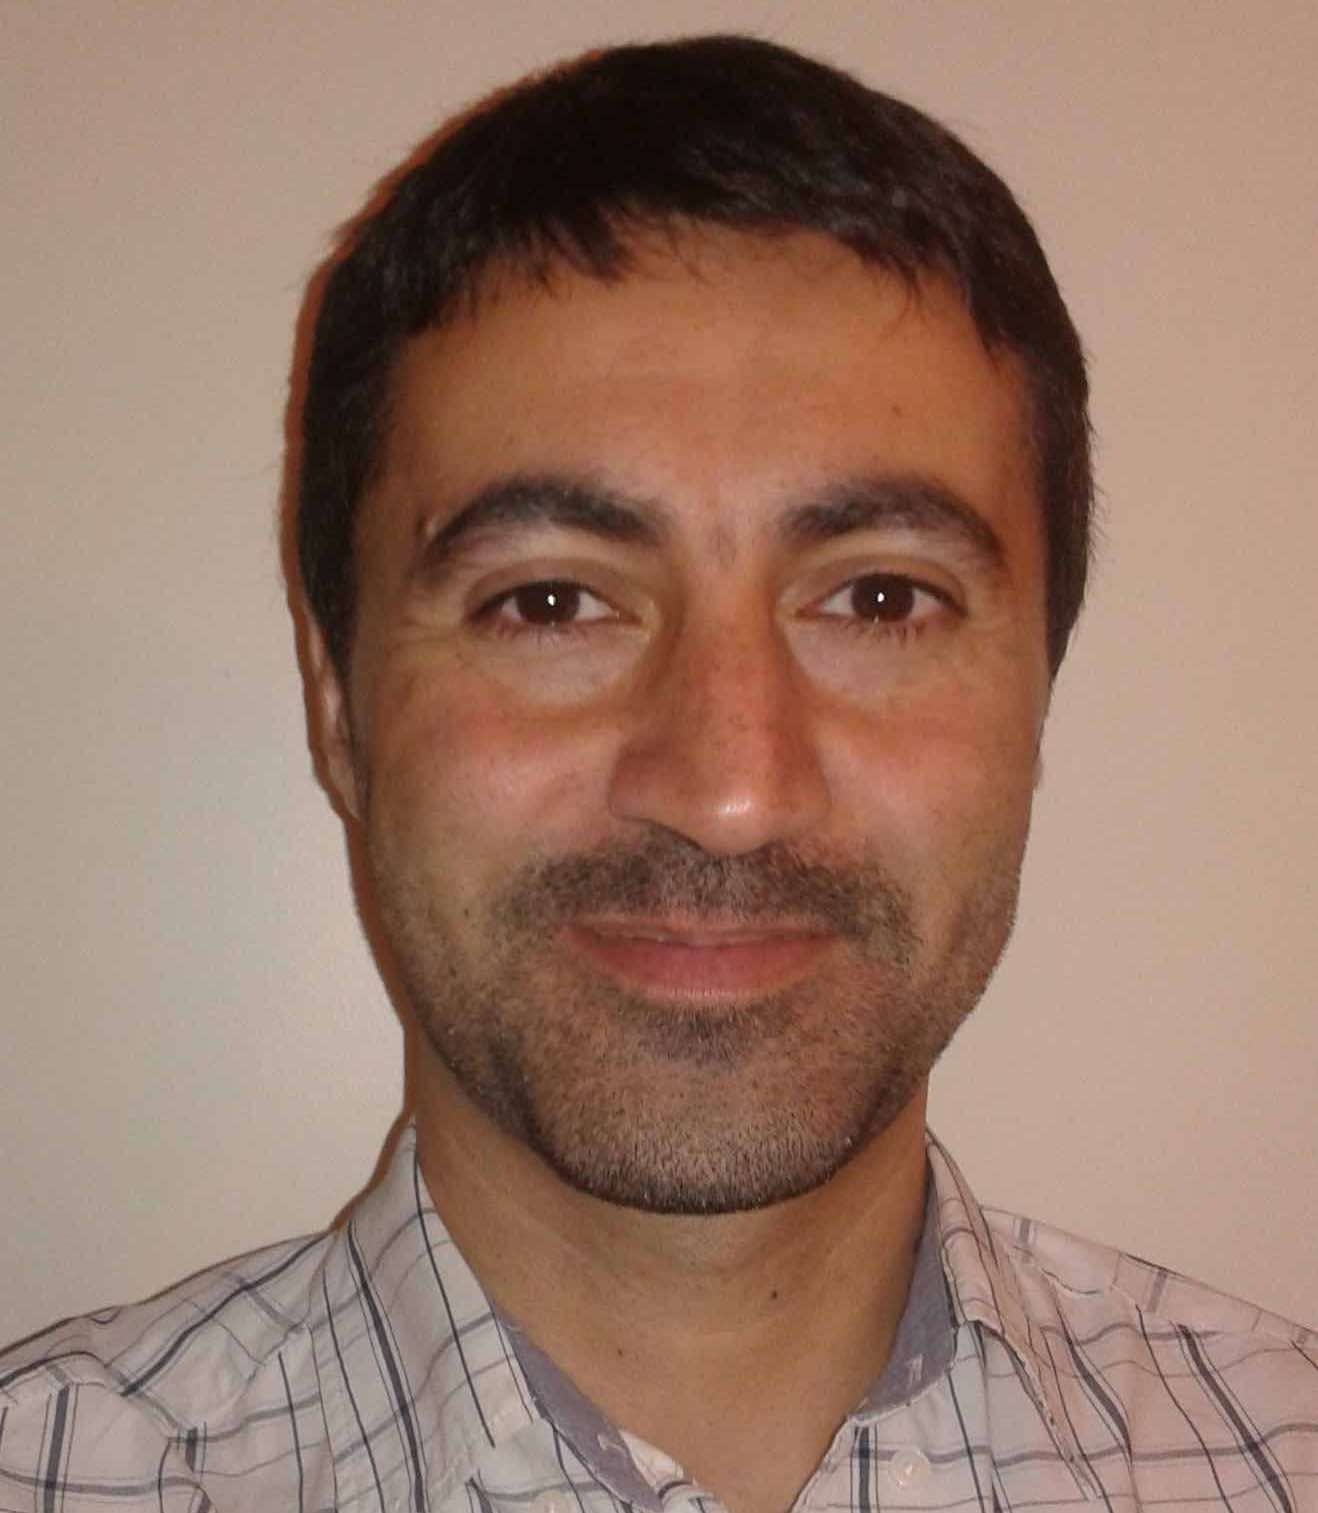
\includegraphics[width=1\linewidth]{anas/photo_cLR_cropped.jpg}
\end{figure}

\vspace{-10pt}

{\textbf{\large About Dr Anas Batou:}}

\begin{scriptsize}
Dr Anas Batou is member of the Liverpool Insitute for Risk and Uncertainty. He gratuated in “Mechanical Engineering” at {\'E}cole Normale Sup{\'e}rieure de Cachan and {\'E}cole Centrale de Paris in 2005. Anas obtained his PhD  at Université Paris-Est in 2008. From 2008 to 2016, he was assistant professor at Université Paris-Est where he got his Habilitation {\'a} Diriger des Recherches in 2014. In 2015, he obtained a six-months  research associate grant at Centre National de la Recherche Scientific-CNRS. He joined the University of Liverpool in September 2016 as Reader at the School of Engineering, Centre for Materials and Structures.

Anas' research activities are related to: Uncertainty quantification in structural and multibody dynamics, model-order reduction in structural dynamics, vibratory energy mitigation, generation of synthetic accelerograms. His research includes both theoretical aspects and industrial applications in automobile engineering and nuclear civil engineering.

\end{scriptsize}}
%Raphael Moura is a Risk/Regulation Engineering Specialist on leave from the Brazilian Regulator for the Oil & Gas Industry (ANP) since October 2013, when he joined the University of Liverpool’s Institute for Risk and Uncertainty as a PhD candidate. 
%
%He has a Master’s degree in Offshore and Ocean Technology (Cranfield University, UK), a Master of Business Administration (FGV-RJ, Brazil), a postgraduate diploma in Offshore Systems Engineering (UFRJ, Brazil) and a Bachelor’s degree in Production Engineering (CEFET-RJ, Brazil). Mr. Moura joined the Brazilian regulator in November 2005, being appointed by the ANP’s Board of Directors as General Manager for Operational Safety in April 2007. He has been dealing with safety inspections, audits and incident investigations at onshore and offshore oil & gas facilities, and played a central role on the establishment of the risk-based safety regulatory framework in Brazil.
\centerline {\rule{1\linewidth}{.25pt}} % Horizontal line
\begin{scriptsize}
anas.batou@liverpool.ac.uk%\\
\end{scriptsize}

\BackToContents % Link back to the contents of the newsletter

\end{mdframed}\hfill
\end{minipage}
\hspace{0.01\textwidth}
\begin{minipage}[!t]{.75\linewidth}




%\vspace{5pt}
%\includegraphics[width=0.3 \textwidth]{../../issue_1/bruno/nnl-site-logo.png}
%\includegraphics[width=0.2 \textwidth]{../../issue_1/bruno/Page-1.png}

\begin{multicols}{2} % Two-column layout
This Young Investigator project funded by the French National Research Agency (ANR) focuses on the dynamical behaviour of complex structures having a high modal density from the low- to the high-frequency band. As an example, an automobile may have about 20,000 elastic modes in the band [0, 2000] Hz. Two main problems arise when trying to construct a computational model for these structures. 

The first one concerns the construction of a low-dimension Reduced-Order Model (ROM), the use of the classical elastic modes being clearly prohibited for complex structures. The second problem is related to the presence, in the computational model, of inherent uncertainties that increase with the frequency. 
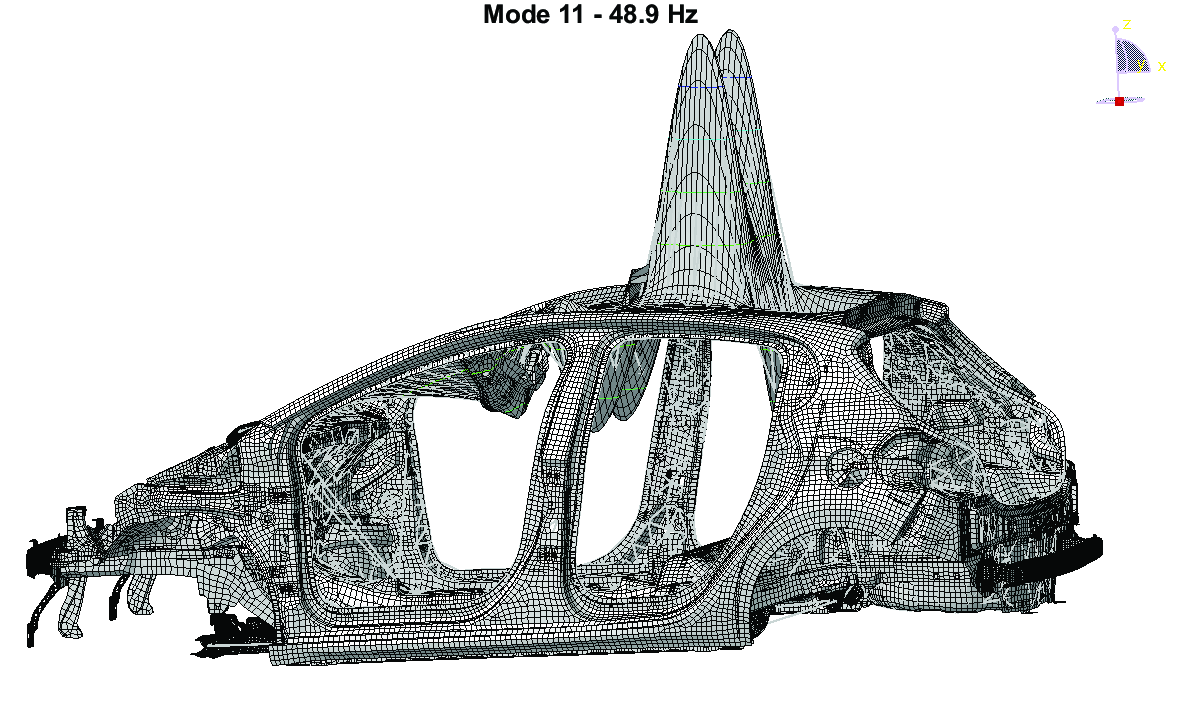
\includegraphics[width=0.5 \textwidth]{anas/fig1.png}
{\scriptsize BIW automobile - Example of global mode belonging to the low-dimension Reduced-Order Basis}\\
%\begin{wrapfigure}[16]{r}[0pt]{0.8 \textwidth}
%\centering
%\includegraphics[width=0.8 \textwidth]{../../issue_1/bruno/figure.jpg}
%\vspace{-40pt}
%\caption{Future plan for Germany's phase out}
%\end{wrapfigure}
In this project, a general  multi-level stochastic ROM (SROM) method has been developed to tackle these issues. It allows the construction of a low-dimension ROM for which the very localized non-contributing displacements are filtered. Furthermore, it allows the stochastic fluctuation related to each low-,  mid- and high-frequency ranges to be controlled separately. This method has been applied to linear as well as non linear structures.
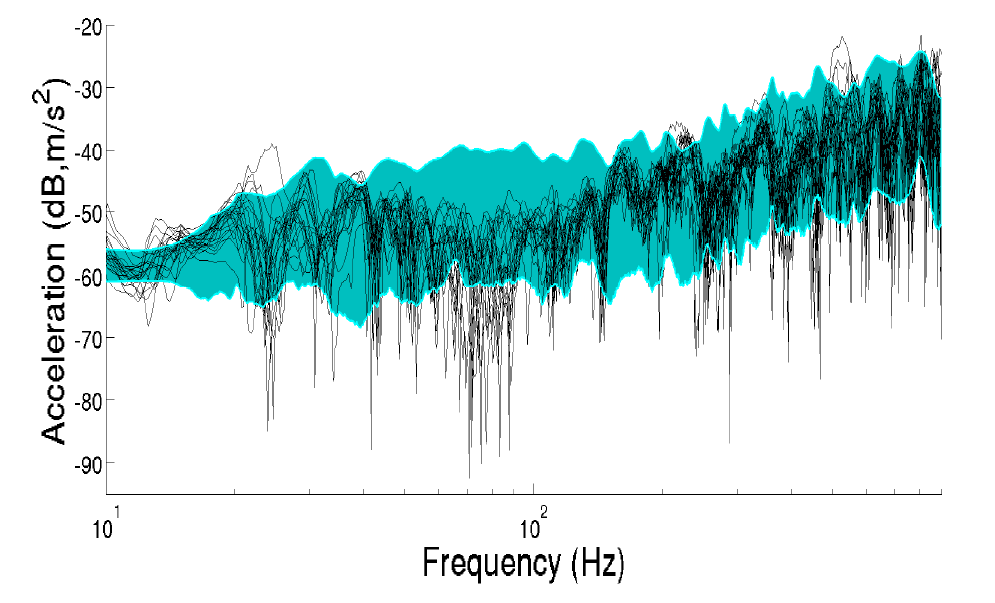
\includegraphics[width=0.5 \textwidth]{anas/fig2.png}
{\scriptsize Experimental FRF measurements (black lines) and random FRF using the SROM (colored region)}\\

In collaboration with the company PSA, 
\begin{wrapfigure}[5]{r}[0pt]{0.2 \textwidth}
\vspace{-10pt}

\includegraphics[width=0.16 \textwidth]{anas/logoLR.jpg}
\end{wrapfigure}
a SROM of an automobile has been constructed and the parameters of this model have been calibrated using experimental frequency responses measured on 20 vehicles from the same production line. The calibrated SROM allows a good prediction of the random dynamical response in the frequency band [0, 1000] Hz.
%\begin{wrapfigure}[3]{r}[0pt]{0.3 \textwidth}
%\centering
%
%\end{wrapfigure}

This project will terminate at the end of 2016. As possible future research to this project, the coupling of this approach with SEA-like methods could extend the domain of predictability of the  SROM to very large frequencies.
\end{multicols}
\end{minipage}

















\cleardoublepage

\thispagestyle{studentProjects}

\begin{minipage}[t]{.99\linewidth} % Mini page taking up 66% of the actual page
\hypertarget{Lauren}{\heading{Becoming an Expert: Lauren Swan on informing risk during an emergency}{6pt}}
%\vspace{-10pt}
%\begin{figure}[H]
%\centering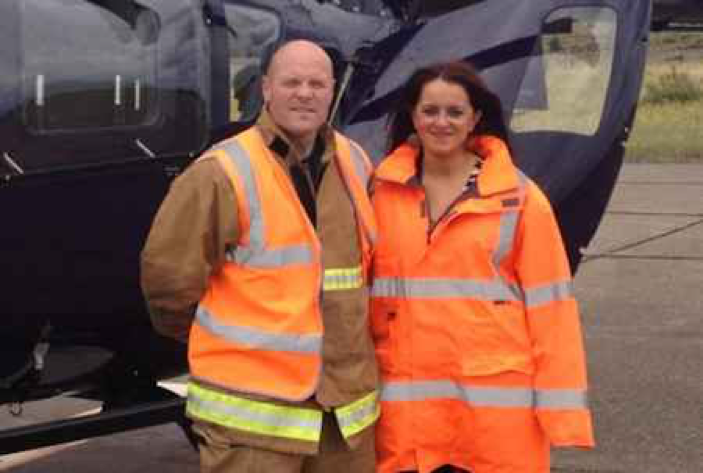
\includegraphics[width=0.9\linewidth]{lauren/laurenFireRescue.png}
%\end{figure}
\end{minipage}


{\bf Lauren Swan}, \textit{PhD Student, year three}\\
\textit{Supervisors}: Laurence Alison \footnote{Professor of Psychological Sciences, Chair in Forensic Psychology, Institute for Risk and Uncertainty, University of Liverpool, UK}, Michael Beer\footnote{Professor and Head: Institute for Computer Science in Civil Engineering, Leibniz University, Hannover, Germany}, Sara Waring\footnote{Lecturer, School of Psychology, Institute for Risk and Uncertainty, University of Liverpool, UK}\\


\begin{minipage}{.75\linewidth}
\begin{multicols}{2} % Two-column layout
Contrary to popular belief, it is uncommon for people to panic or act irrationally during an emergency. However, their behaviour can be unpredictable due to their lack of familiarity with the situation. It is therefore essential that casualties be given clear, concise and direct instructions during emergencies, although this is rarely at the forefront of emergency service training.

Thanks to the partnership between the University of Liverpool’s Department of Psychological Sciences, Merseyside Fire and Rescue Service and London Fire Brigade, I have had the opportunity to collect data from responders and casualties in numerous multi-agency training events.

Over the course of my PhD I have been in the unique position of being able to explore casualty perceptions and experiences within a number of national large scale, live, multi-agency exercise involving police, fire and ambulance and their partner agencies.

The first large scale exercise, known as 'Joint Endeavour', involved a train derailing from the tracks and colliding with a building, several vehicles and power lines, which in turn caused a bus to crash into a learning centre. The second large scale exercise, known as ‘Unified Response’, involved a building collapse on Waterloo tube station, which in turn injured hundreds of people. 

Members of the public, Amputees in Action and professional actors played the role of casualties and concerned family members in both exercises to add a level of realism for the  hundreds of practitioners who took part.

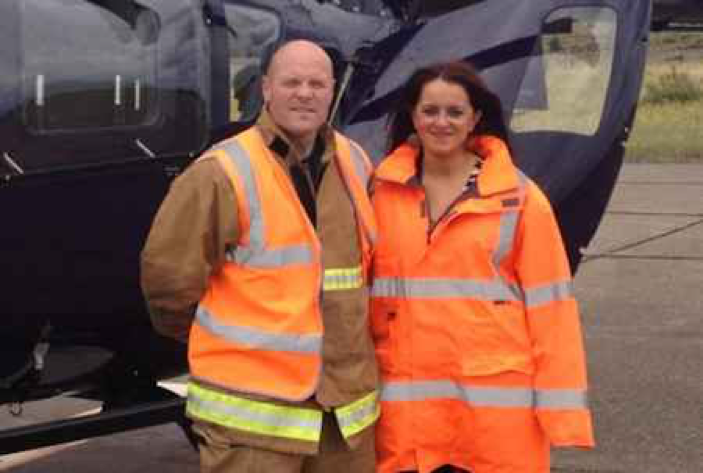
\includegraphics[width=0.5 \textwidth]{lauren/laurenFireRescue.png}\\
{\scriptsize Lauren Swan with Chief Fire Officer Dan Stephens of Merseyside Fire and Rescue Service}


Data was collected in the form of pre- and post-event surveys and post-event interviews, which provided a rich, in-depth account of casualty perceptions of how the emergency services interacted with them and how it felt to be a casualty.

This will feed into the work I am conducting to understand public preferences in relation to risk communication in order to aid in the production of adequate guidelines for risk communication training.

In addition to communicating risk information effectively at the acute end of an emergency, informing the public of potential risks and helping them to be prepared in advance can be very useful.

To be better informed and prepared for local emergencies, take a look at the Merseyside Prepared website: www.merseysideprepared.org.uk. 



\end{multicols}
\end{minipage}
\hspace{0.01\textwidth}
\begin{minipage}{.25\linewidth}
\begin{mdframed}[style=about,frametitle={}] % Sidebar box
%\begin{figure}[H]
%\includegraphics[width=1\linewidth]{lauren/profPict.jpg}
%\end{figure}

{\textbf{\large About Lauren:}}
%\hypertarget{About Petra:}{0pt}

\begin{footnotesize}
Lauren is in the third year of a full time interdisciplinary PhD with the Critical and Major Incident Research group in the Department of Psychological Sciences and the Liverpool Institute of Risk and Uncertainty. 

``The purpose of my PhD research is to identify the most effective ways to communicate risk to the public during an emergency. This is still a fairly novel area of research despite the number of high profile major disasters that have occurred over the last 30 years, such as Fukushima, and the evidence that ineffective risk communication can result in potentially fatal consequences.''

``I have been working with the MRF to develop a website that contains the type of risk and preparedness information that members of the public want to receive. This feedback has been utilised by the MRF to implement appropriate changes before the website went live on 30th October 2014.''

I have also gathered a wider range of public perceptions on the type of information that should be presented in advance of emergencies and how the public can best be helped to be prepared by carrying out a short on-line survey.
\end{footnotesize}

\centerline {\rule{1\linewidth}{.25pt}} % Horizontal line

\begin{scriptsize}
%For more details: \\
L.C.Swan@liverpool.ac.uk \\
%See more on the LIRU website
\end{scriptsize}
\BackToContents % Link back to the contents of the newsletter
\end{mdframed}\hfill
\end{minipage}

%\begin{minipage}{0.99 \linewidth}


%Emergency service resources are finite and the public can be empowered to help themselves and their families, thereby reducing some of the pressure on emergency services and enabling them to use resources more effectively to save lives.

%This is one of the concerns of the Merseyside Resilience Forum (MRF), which is a multi-agency partnership prescribed within the Civil Contingencies Act 2004 that provides guidance and support to the communities of Merseyside in order to improve community resilience.

%I have been working with the MRF to develop a website that contains the type of risk and preparedness information that members of the public want to receive. My initial contribution was to run focus groups with members of the Merseyside public to attain feedback throughout the development stages of the website in order to identify the type of information the public wanted to receive, the level of detail and how such information should be presented. This feedback has been utilised by the MRF to implement appropriate changes before the website went live on 30th October 2014. 

%I have also gathered a wider range of public perceptions on the type of information that should be presented in advance of emergencies and how the public can best be helped to be prepared by carrying out a short on-line survey, the findings of which have been directly fed back to the agencies within the MRF in order to improve their communication and relationship with the public. 

%To be better informed and prepared for local emergencies, take a look at the Merseyside Prepared website: www.merseysideprepared.org.uk. 


%\end{minipage}
















\cleardoublepage

\thispagestyle{studentProjects}

\begin{minipage}[t]{.90\linewidth} % Mini page taking up 66% of the actual page
\hypertarget{Lauren2}{\heading{Researchers evaluate UK’s largest disaster training exercise}{6pt}}
\vspace{-10pt}
%\begin{figure}[H]
%\centering\includegraphics[width=0.9\linewidth]{lauren/}
%\end{figure}
\end{minipage}


\begin{minipage}{.75\linewidth}
\begin{center}
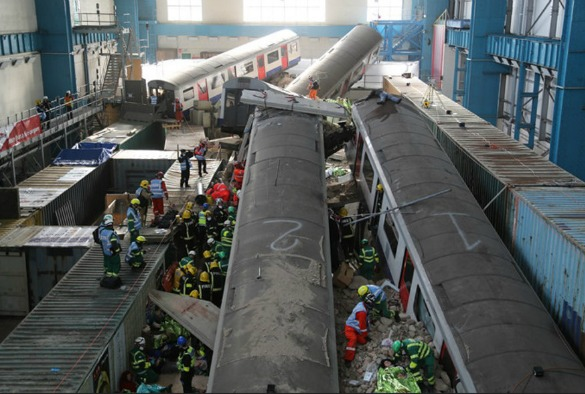
\includegraphics[width=0.98 \textwidth]{lauren/trainDerail.jpg}
\end{center}
{\scriptsize photo by @londonfire}
\begin{multicols}{2}

The University of Liverpool is part of the core team evaluating the largest disaster training exercise ever staged in the UK.

Exercise Unified Response (EUR) was hosted by the London Fire Brigade as part of the EU Civil Protection Mechanism, and involved fire-fighters, police officers and ambulance personnel from across London, the UK and Europe. They took part in a four-day scenario based on a building collapsing onto a major transport hub in the capital. The exercise was designed to test a number of national response frameworks and protocols, but also to test the international cooperation across various EU member states.

\textbf{Observation}\\
To help the emergency services learn from the experience, psychologists from the University’s Critical & Major Incident Psychology (CAMI) research group, from both the Liverpool and London campuses, have been involved throughout the planning and preparation stages of the event. 

The researchers coordinated a number of ’observer’ teams during the live exercise, collecting information on emergency service response, coordination and cooperation, as well as the experience of volunteers playing the part of victims and casualties. The exercise had more than 2,500 casualties, thousands of tonnes of rubble, seven tube carriages and hundreds of emergency service responders.

\textbf{Rescue teams}\\
The major operation involved over 4,000 emergency responders, including 300 responders from European specialist rescue units, representatives from local authorities and other assistance services. 
Dr Michael Humann\footnote{Centre for Critical \& Major Incident Psychology Research, School of Psychology} led the 22-strong University team, which included academic colleagues from the Department of Psychology, as well PhD and MSc students on our academic programme.

%The University was invited to assist with the exercise having supported the Joint Emergency Services Interoperability Programme (JESIP) exercise last year in Liverpool that saw a fire service training station turned into a disaster area as part of the national Home Office funded project.

%Essential
%To date, EUR is just one of the areas in which the CAMI research group has worked with emergency services. They have also assisted with a number of other exercises around Merseyside and the UK, while also developing long-term training and learning programmes.

%More information about CAMI can be found here.

\end{multicols}






\end{minipage}
\hspace{0.01\textwidth}
\begin{minipage}{.25\linewidth}
\begin{mdframed}[style=about,frametitle={}] % Sidebar box
\begin{figure}[H]

\includegraphics[width=1\linewidth]{lauren/humannProfPic.jpg}
\end{figure}

{\textbf{ Dr Michael Humann:}}
%\hypertarget{About Petra:}{0pt}

\begin{small}
``These types of exercises are essential to help emergency services respond quickly and effectively to large scale disasters.

Our team has not only been involved in the evaluation, but have also assisted in the planning of this complex large scale disaster simulation, ensuring a rich experience for the responders as well as the volunteering public. 

We are evaluating everything from the command structure to how individual units communicate with one another. This is crucial to help individuals and the services involved perform better in a real crisis. 

Similarly, we are also capturing the public’s experience of their interaction with the various agencies, as well as their overall perceptions of how the emergency services and other authorities train and prepare for such incidents, so as to improve the engagement and information exchange in the future.''

\end{small}

\centerline {\rule{1\linewidth}{.25pt}} % Horizontal line

\begin{scriptsize}
%For more details: \\
M.Humann@liverpool.ac.uk%\\
%See more on the LIRU website
\end{scriptsize}
\BackToContents % Link back to the contents of the newsletter
\end{mdframed}\hfill
\end{minipage}














\cleardoublepage

\thispagestyle{studentProjects}

\begin{minipage}[t]{.99\linewidth} % Mini page taking up 66% of the actual page
\hypertarget{Simon}{\heading{Risk of river flood inundation from vegetation change under climate change
}{6pt}}
\end{minipage}

{\bf Simon Clark}, \textit{PhD CDT Student, year one}\\
\textit{Supervisors}: James R. Cooper \footnote{Lecturer, School of Environmental Sciences, University of Liverpool}, Ming Li\footnote{School of Engineering, University of Liverpool}, Janet Hooke\footnote{Professor, School of Environmental Sciences, University of Liverpool}, Ponnambalam Rameshwaran\footnote{Centre for Ecology and Hydrology, UK}\\

\vspace{-10pt}

\begin{minipage}[t]{.24\linewidth}
\vspace{10pt}
\begin{mdframed}[style=about,frametitle={}] % Sidebar box

\begin{figure}[H]
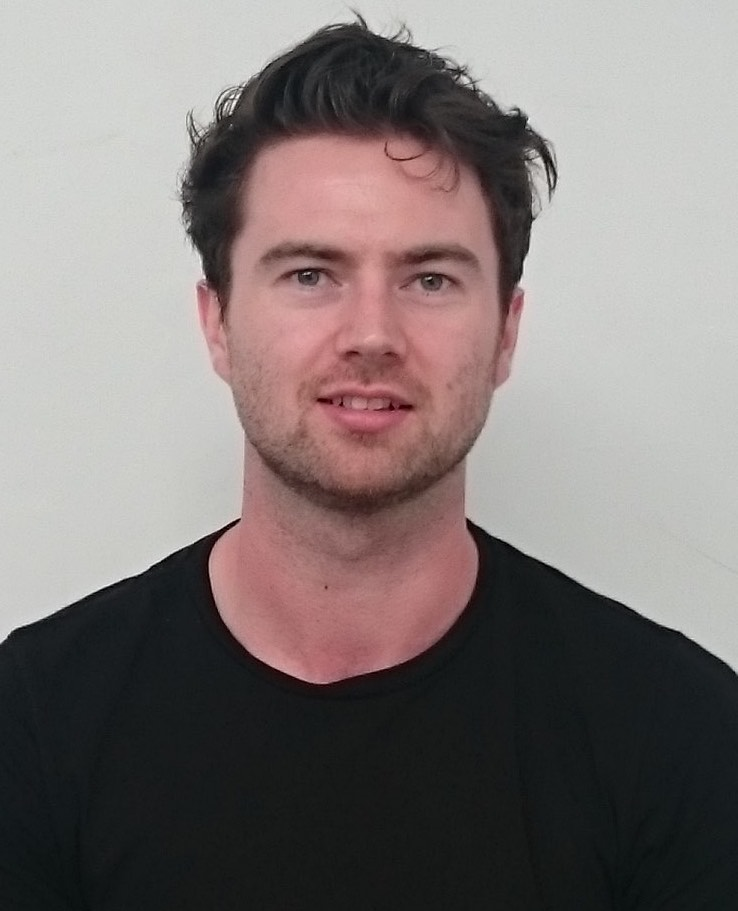
\includegraphics[width=1\linewidth]{simon/simonPict.jpg}
\end{figure}

\vspace{-10pt}

{\textbf{\large About Simon:}}

\begin{scriptsize}

I first studied Geography BSc at the University of Manchester. My studies allowed me to work in public and industrial positions, working at Natural England and hydrological consultancy Cascade Consulting. I returned to academia and studied an MSc in Environmental Modelling, Monitoring, and Reconstruction at the University of Manchester, before undertaking my current PhD in Liverpool. As a researcher I have always had a vested interest in hydrology, from policy and ecology to its cultural presence, however my core passion is flood risk mitigation.

Current research lacks a comprehensive model for estimating the effect of vegetation flow response on flood risk. This is further complicated by the complex and diverse factors involved in river flooding, such as climate gradients, dominant vegetation species, and river morphology. As such, including vegetation in flood models may allow for greater accuracy in flood prediction.

\end{scriptsize}
\centerline {\rule{1\linewidth}{.25pt}} % Horizontal line
\begin{scriptsize}
%For more details: \\
sdaclark@liverpool.ac.uk
%\BackToContents % Link back to the contents of the newsletter
\end{scriptsize}

\end{mdframed}\hfill
\end{minipage}
\hspace{0.01\textwidth}
\begin{minipage}[t]{.75\linewidth}

\vspace{1pt}
\begin{multicols}{2} % Two-column layout

%\vspace{-15pt}
%\begin{wrapfigure}[3]{r}[0pt]{0pt}
%\includegraphics[width=0.25\linewidth]{../peterHristov/park.PNG} 
%\end{wrapfigure}

The impacts of climate change are predicted to adversely affect human populations, therefore predicting changes in flood risk is vital for developing adaptive measures. In the UK, concern over river flooding have been exacerbated by recent flooding events and the projected increases in climatic pressures on river flow. An increasing collection of research suggests that interactions between in-stream vegetation and flow conveyance reduces both river velocity and river capacity, increasing local river depth. %This exaggerates local flood risk to populations near vegetated rivers, however it also opens up the possibility for localised flood storage to control flood risk downstream. 


%\end{minipage}
%\vspace{-15pt}


This project aims to enhance river flood prediction by accounting for the effects of in-stream vegetation. Vegetation has so far been absent from hydraulic models and may account for a considerable degree of uncertainty in flood predictions. Previous studies using 2D models have elucidated relationships between vegetation and flow, however 2D approaches are limited due to the 3D nature of plant profiles in the water column, and their agency in turbulence generation. The problem is further complicated by species-specific plant morphology (such as leaf shape and stem flexibility, respectively).% and growing seasons resulting in different effects on flow throughout the year. Climate change is set to alter growing seasons, as well as the intensity and frequency of rainfall, adding another layer of complexity.

To capture the effect of plant-flow dynamics a 3D model must be adopted. Current hydraulic approaches generally favour Reynolds-averaged Navier-Stoke equations (RANS). RANs are used in anisotropic turbulence models with one or multi-equation approaches, and are used to resolve local flow and turbulence induced features through a time-averaged flow field. Flow over or through vegetation can be predicted with RANS models by adding additional source terms to the RANS and turbulence transport equations to account for vegetative drag effects. RANS also offer a practical approach, offering reasonable accuracy of the time-averaged turbulent flow field.

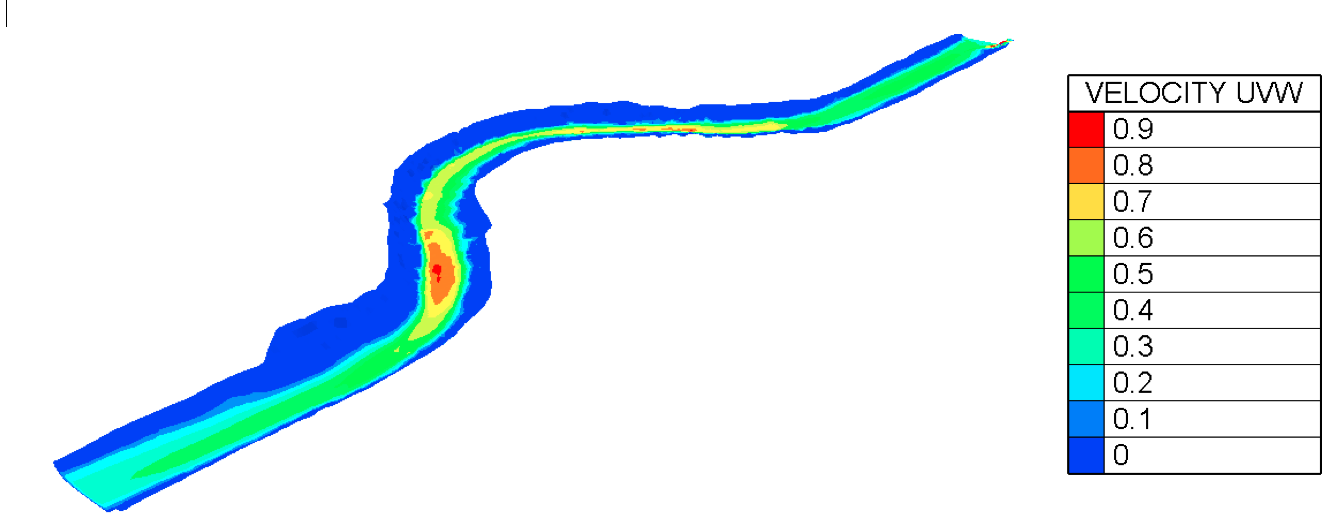
\includegraphics[width=1\linewidth]{simon/projectPict.png}
{\scriptsize Simulation of streamwise velocity (m/s) using Telemac 3D in the River }

The project uses TELEMAC 3D, a processing chain for three-dimensional free surface flow for the calculation of water in rivers. TELEMAC was chosen for three reasons: firstly, it is able to model river flooding effectively, solving full 3D non-hydrostatic RANS equations with a free surface; 
secondly, it’s ubiquitous in research and industry, positioning the research project to operate on a field similar to that of other professionals; thirdly, as an open-source model it freely allows for the addition of subroutines to specify complex and important flow phenomena – important for the integration of vegetation in the flood prediction model.

%The premise behind the educational campaigns is that a poor understanding of dog body language leads to greater risk-taking behaviours around dogs. Therefore, education in dog behaviour will decrease the number of bites. However, a recent study indicated that individuals often perceive dog bites as unavoidable, which may pose a barrier to instilling changes in their behaviour around dogs and the effectiveness of education.  
%\begin{wrapfigure}[4]{r}[0pt]{0pt}
%\includegraphics[width=0.2\linewidth]{../../issue_1/sara/royal_trust.png}
%\end{wrapfigure}
%To date, most research around dog bites uses traditional epidemiological approaches (11), which have not offered many insights into differences in individuals' perceptions of bites. Applying qualitative approaches to the study of bites, and in particular, using sociological models of risk is a novel and exciting way to approach this problem. 
\end{multicols}
\end{minipage}




\cleardoublepage













%\thispagestyle{IPW}

%\begin{minipage}[t]{.50\linewidth} % Mini page taking up 66% of the actual page
%%-----------------------------------------------------------
%
%\hypertarget{IPW}{\heading{LIRU hosts and organises the 13$^{\text{th}}$ International Probabilistic Workshop (IPW 2015)}{6pt}} % \hypertarget provides a label to reference using \hyperlink{label}{link text}

%The workshop has taken place in Liverpool, UK, from 4${^\text{th}}$ to 6${^\text{th}}$ of November at the University of Liverpool. IPW2015 has provided a multi-disciplinary forum for the exchange of knowledge and expertise, in the probabilistic methods, uncertainty quantification, safety and risk management.
%Overall, the conference programme consisted of 46 presentations and 5 keynote lectures by invited internationally renowned researchers. Around 100 delegates from 18 countries attended the workshops. \href{http://rpsonline.com.sg/rps2prod/ipw2015/index.html}{Proceedings} are freely available and can be downloaded at \href{http://ipw2015.org/}{http://ipw2015.org/}.

%The event was aimed at specialised and synergetic developments in both theory and practice. %Both industry and academia were invited to contribute and to join in the discussions on developments and needs in the field.

%This joint conference has been organised by the Institute for Risk \& Uncertainty. In the previous years a series of probabilistic workshops on safety and risk were organised starting in 2003.

%Next year the 14${^\text{th}}$ edition of the IPW event will take place at the Ghent University in Belgium.

%\end{minipage} % End the main body - first page mini page
%\begin{minipage}[t]{.50\linewidth} % Mini page taking up 66% of the actual page
%%-----------------------------------------------------------
%

%\vspace{-15pt}
%\begin{figure}[H]
%\includegraphics[width=0.95\linewidth]{../IPW/draw_1_3.png}
%\end{figure}
%\end{minipage} % End the main body - first page mini page

%\begin{minipage}[b]{0.99\linewidth}
%\vspace{-30pt}
%\centering
%\includegraphics[width=1\linewidth]{../IPW/draw_2_3.png}
%\end{minipage}














\cleardoublepage


\thispagestyle{Training}

\begin{minipage}[t]{0.99\textwidth}
\hypertarget{Training}{\heading{EPSRC \& ESRC Centre for Doctoral Training (CDT) in Risk and Uncertainty}{6pt}}
\end{minipage}

%\begin{center}
{\LARGE Uncertainty Quantification Training Course on HPC with COSSAN}\\
{\large 4$^{\text{th}}$, 5$^{\text{th}}$ and 6$^{\text{th}}$ May 2016, Warrington, UK}
%\end{center}

%{\LARGE Uncertainty Quantification Training Course on HPC with COSSANsoftware,  May 2016}

\begin{figure}[H]
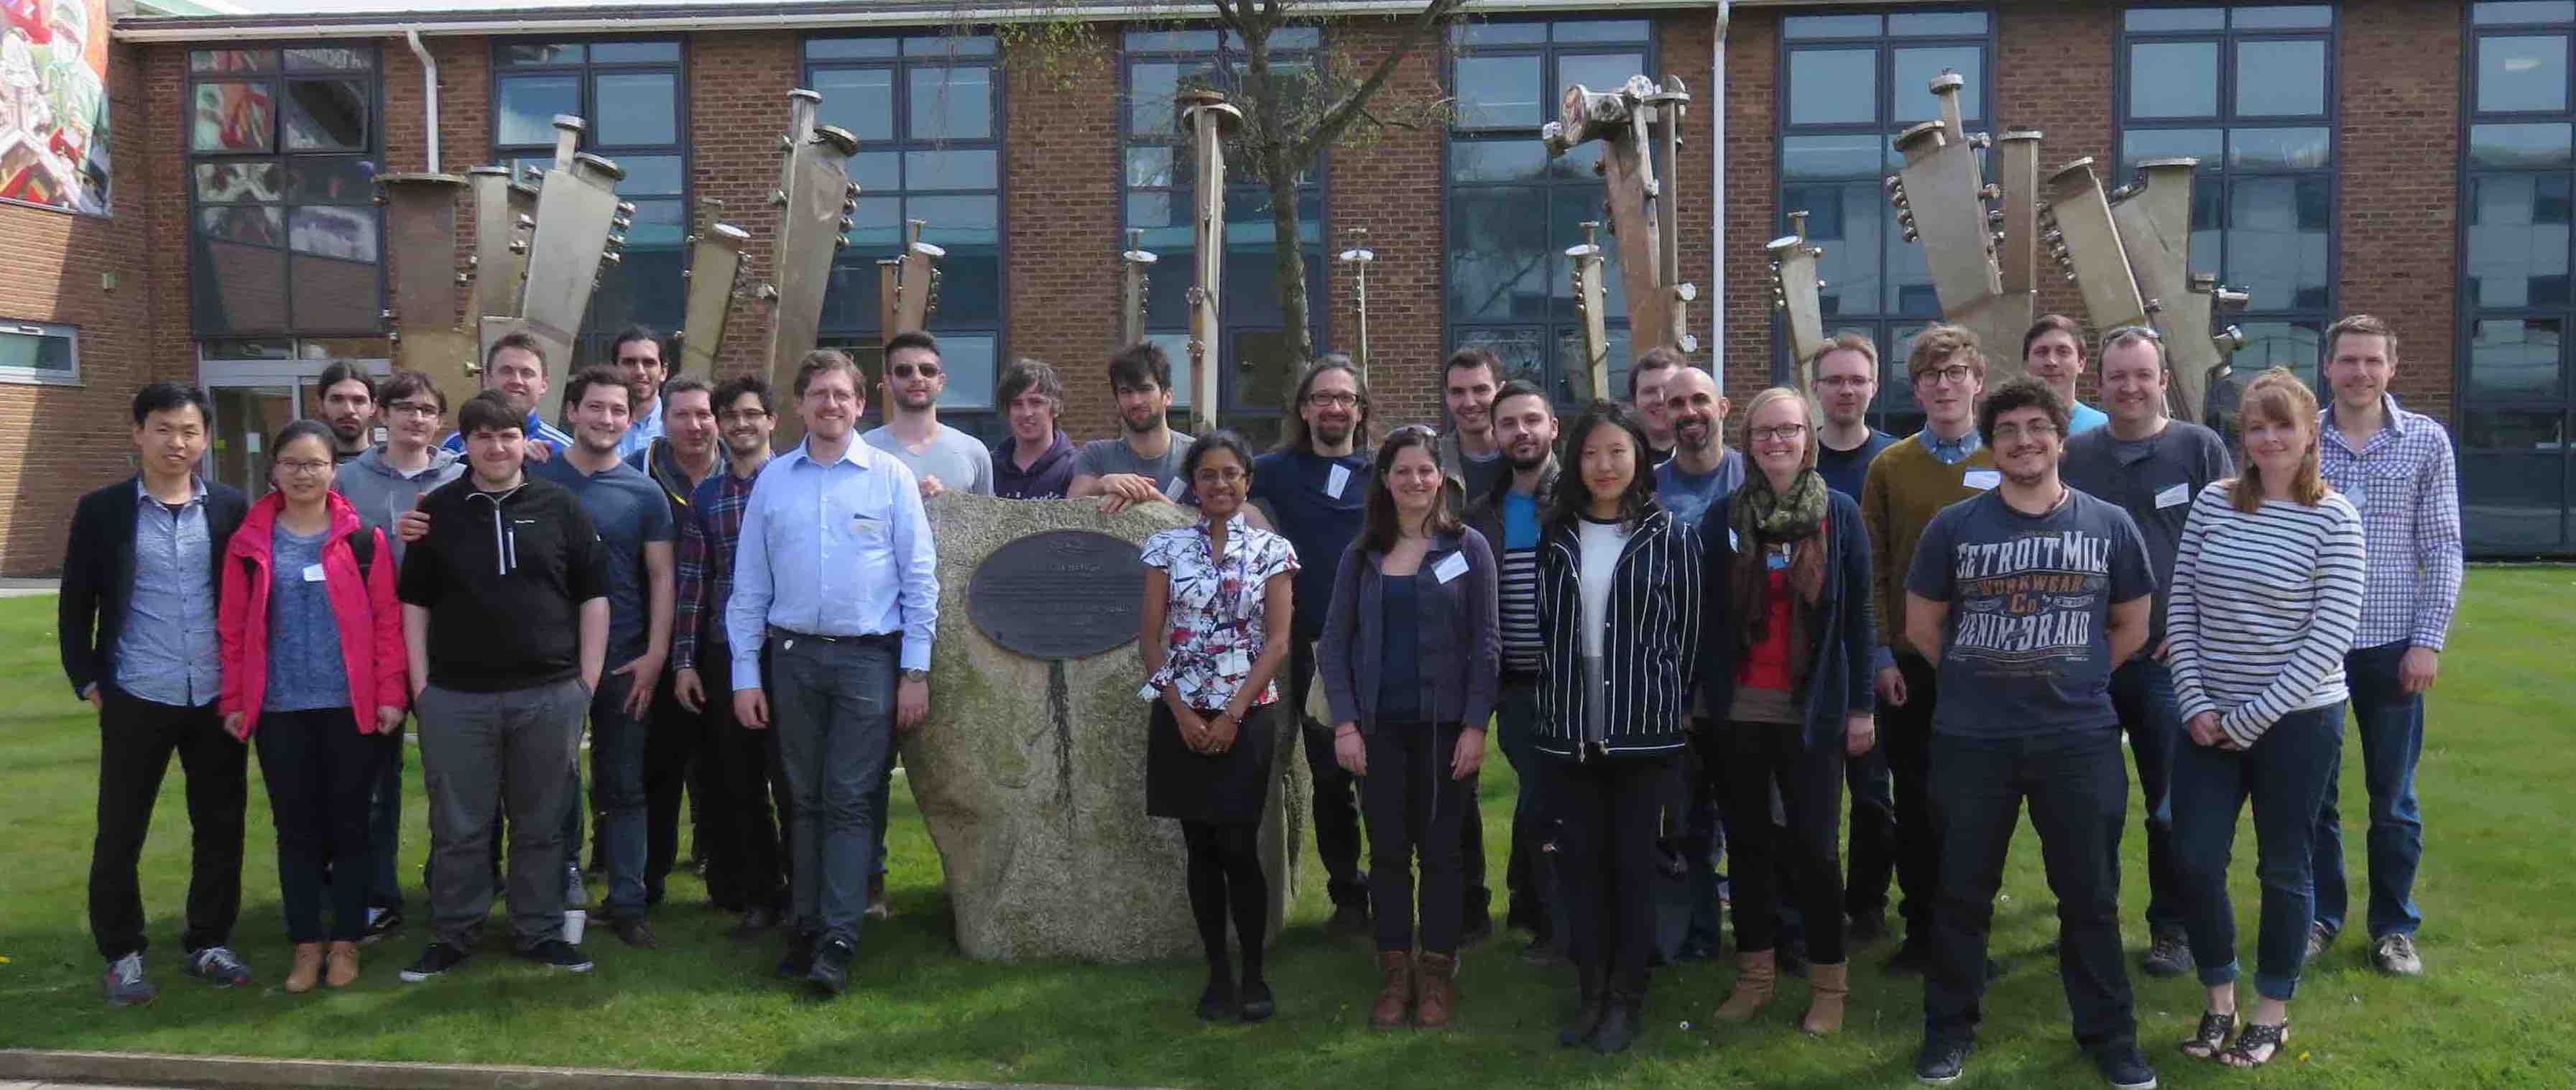
\includegraphics[width=0.95\linewidth]{training/groupPicture_lr.jpg}
%\caption{Group picture}
\end{figure}

\begin{center}
{\Large \color{blue} ``Uncertainty Quantification using COSSAN Software on High Performance Computing''}
\end{center}
%\vspace{10pt}

\begin{minipage}{0.6\textwidth}
{\bf Event Details}\\
In collaboration with the Institute for Risk and Uncertainty and Hartree Centre, a 3 days training course on Uncertainty Quantification using COSSAN Software on High Performance Computing has been offered. The Course took place - Wednesday 4th May 2016 - at STFC Daresbury Laboratory \href{http://maps.google.com/maps?f=q\&source=s_q\&hl=en&geocode=\&q=Daresbury+Innovation+Centre+Warrington+WA4+4FS+United+Kingdom}{(Science and Technology Park)}, in Warrington, Cheshire. Transportation from the University to the Science Park as well as lunch have been provided to all participants charging a small fee (\pounds 50). The list of participants can be seen on the event  \href{https://eventbooking.stfc.ac.uk/news-events/cossan-software}{webpage}.
\end{minipage}
\begin{minipage}{0.39\linewidth}
\begin{center}
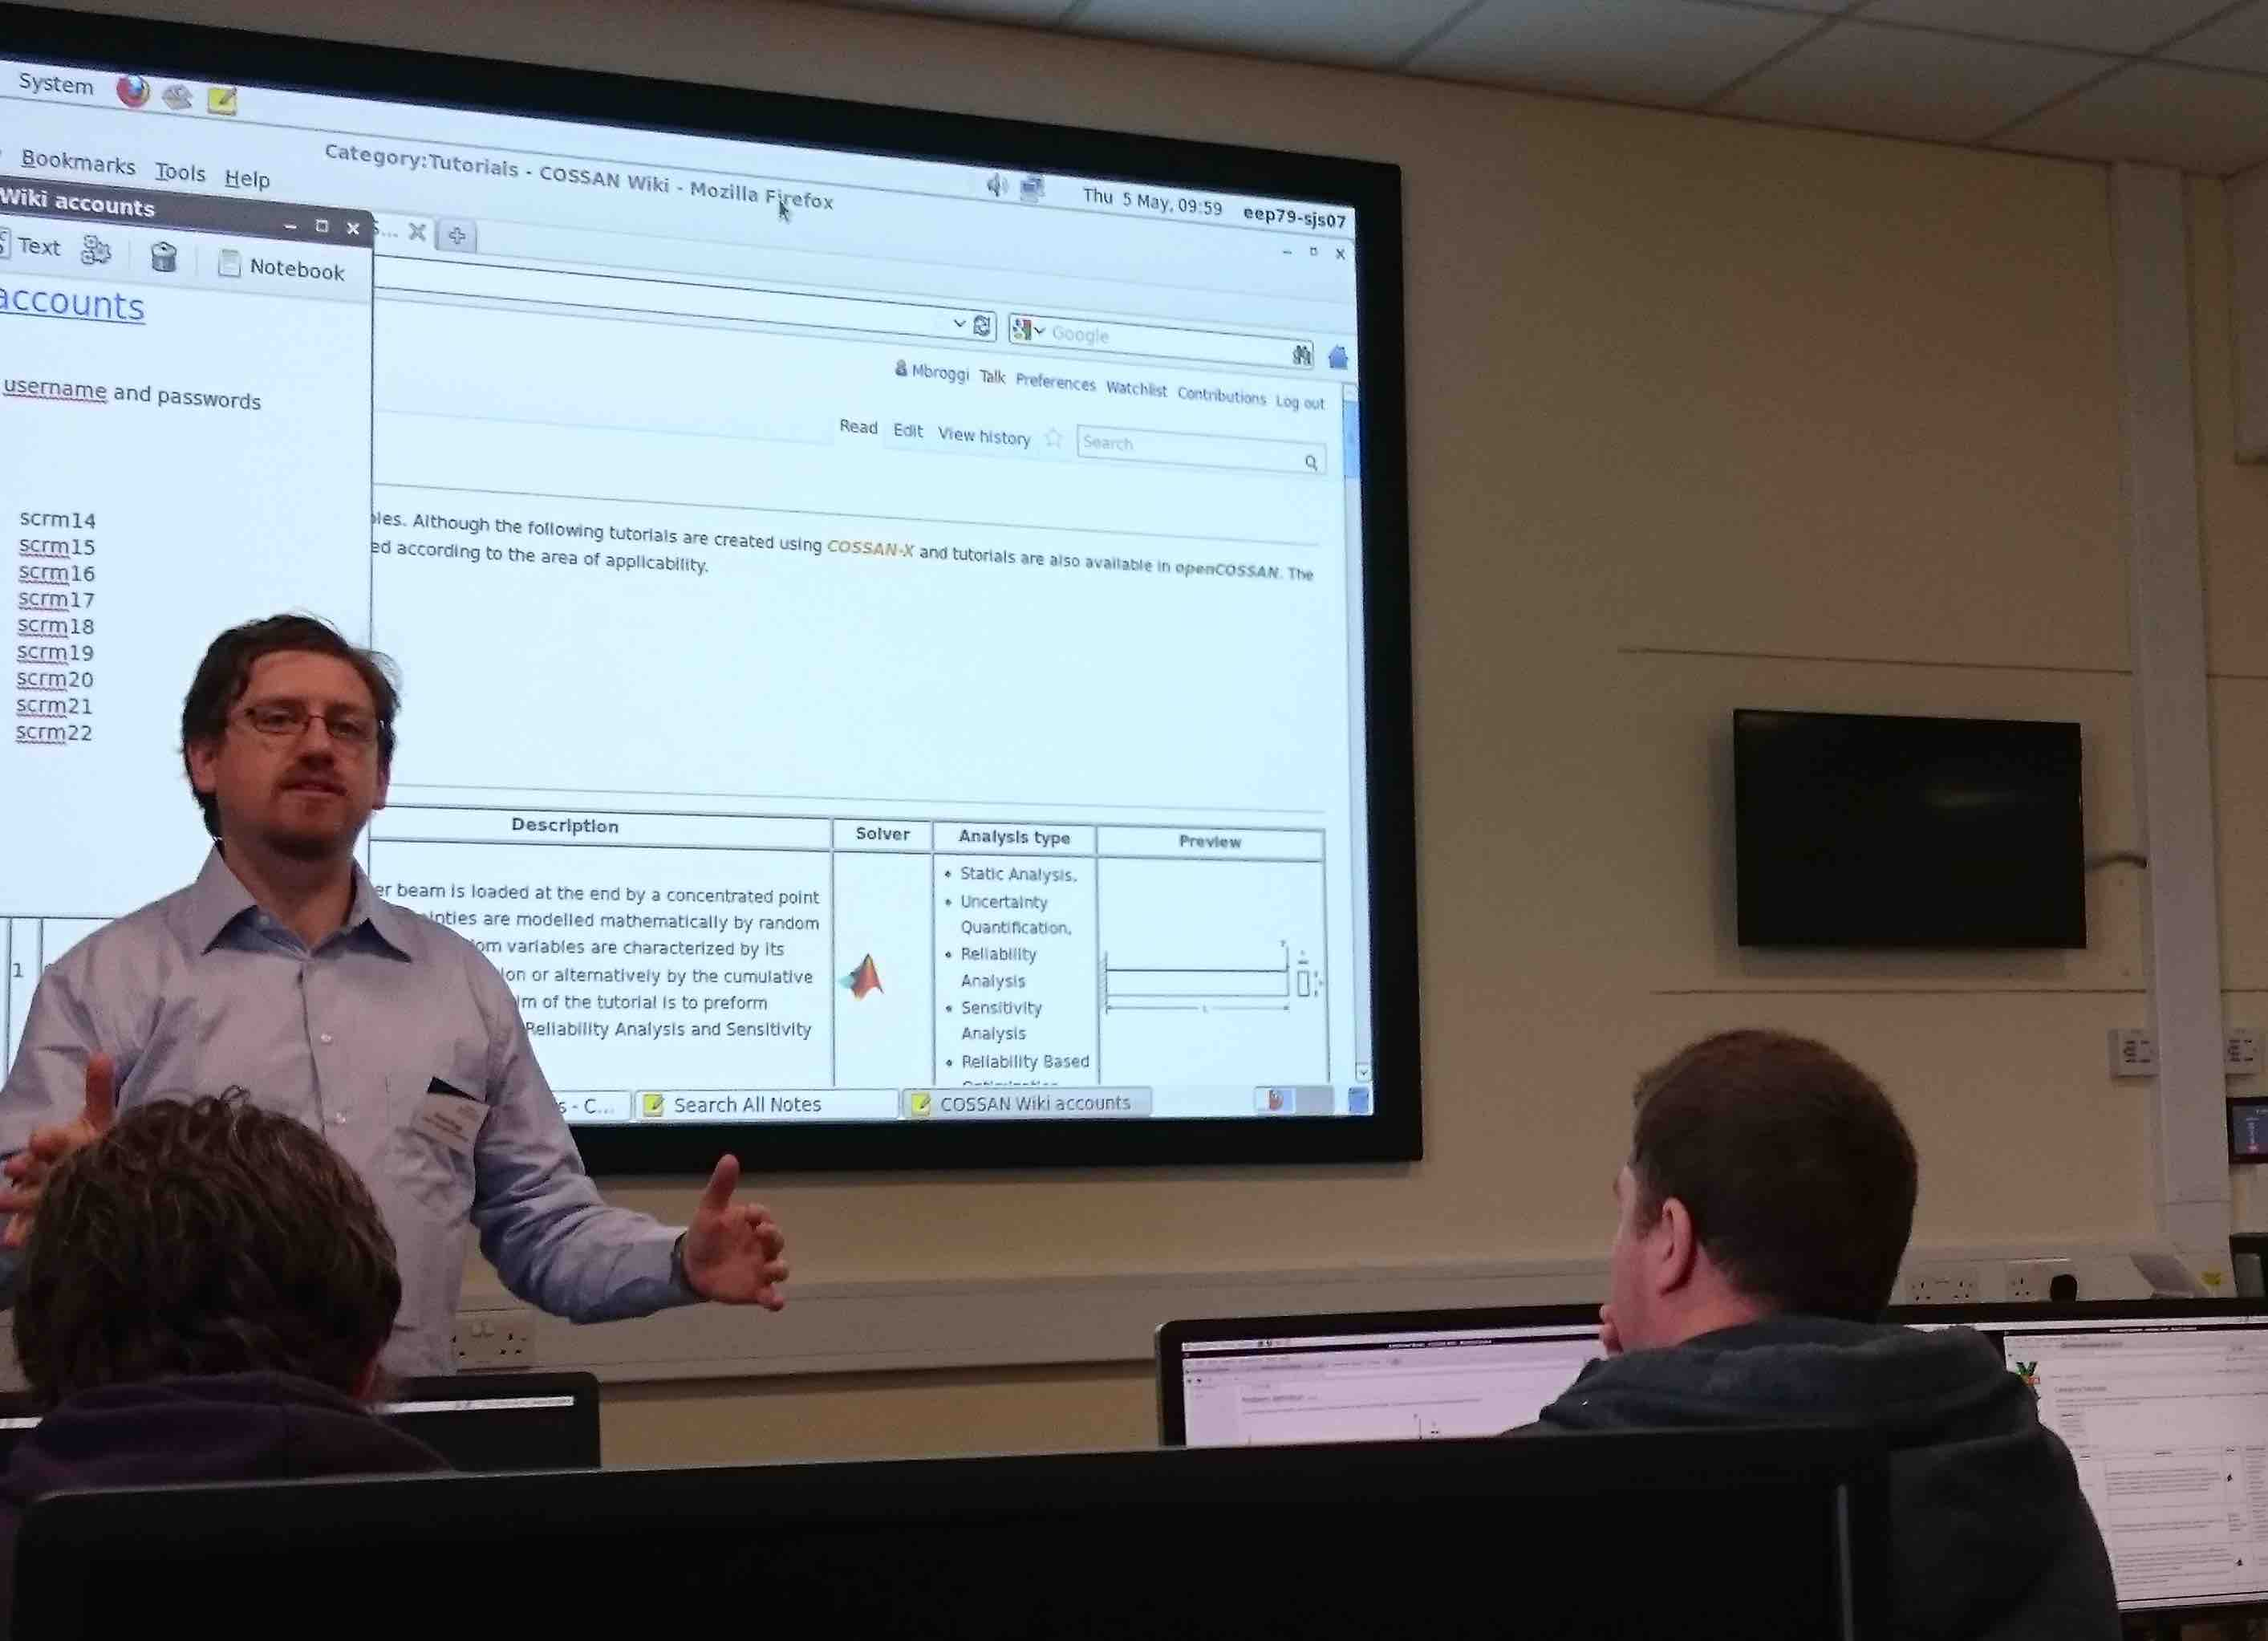
\includegraphics[width=0.95\linewidth]{training/matteo3_lr.jpg}\\
{\small Dr Matteo Broggi - Leibniz University of Hannover}
\end{center}
\end{minipage}


\begin{minipage}{0.39\linewidth}
\begin{center}
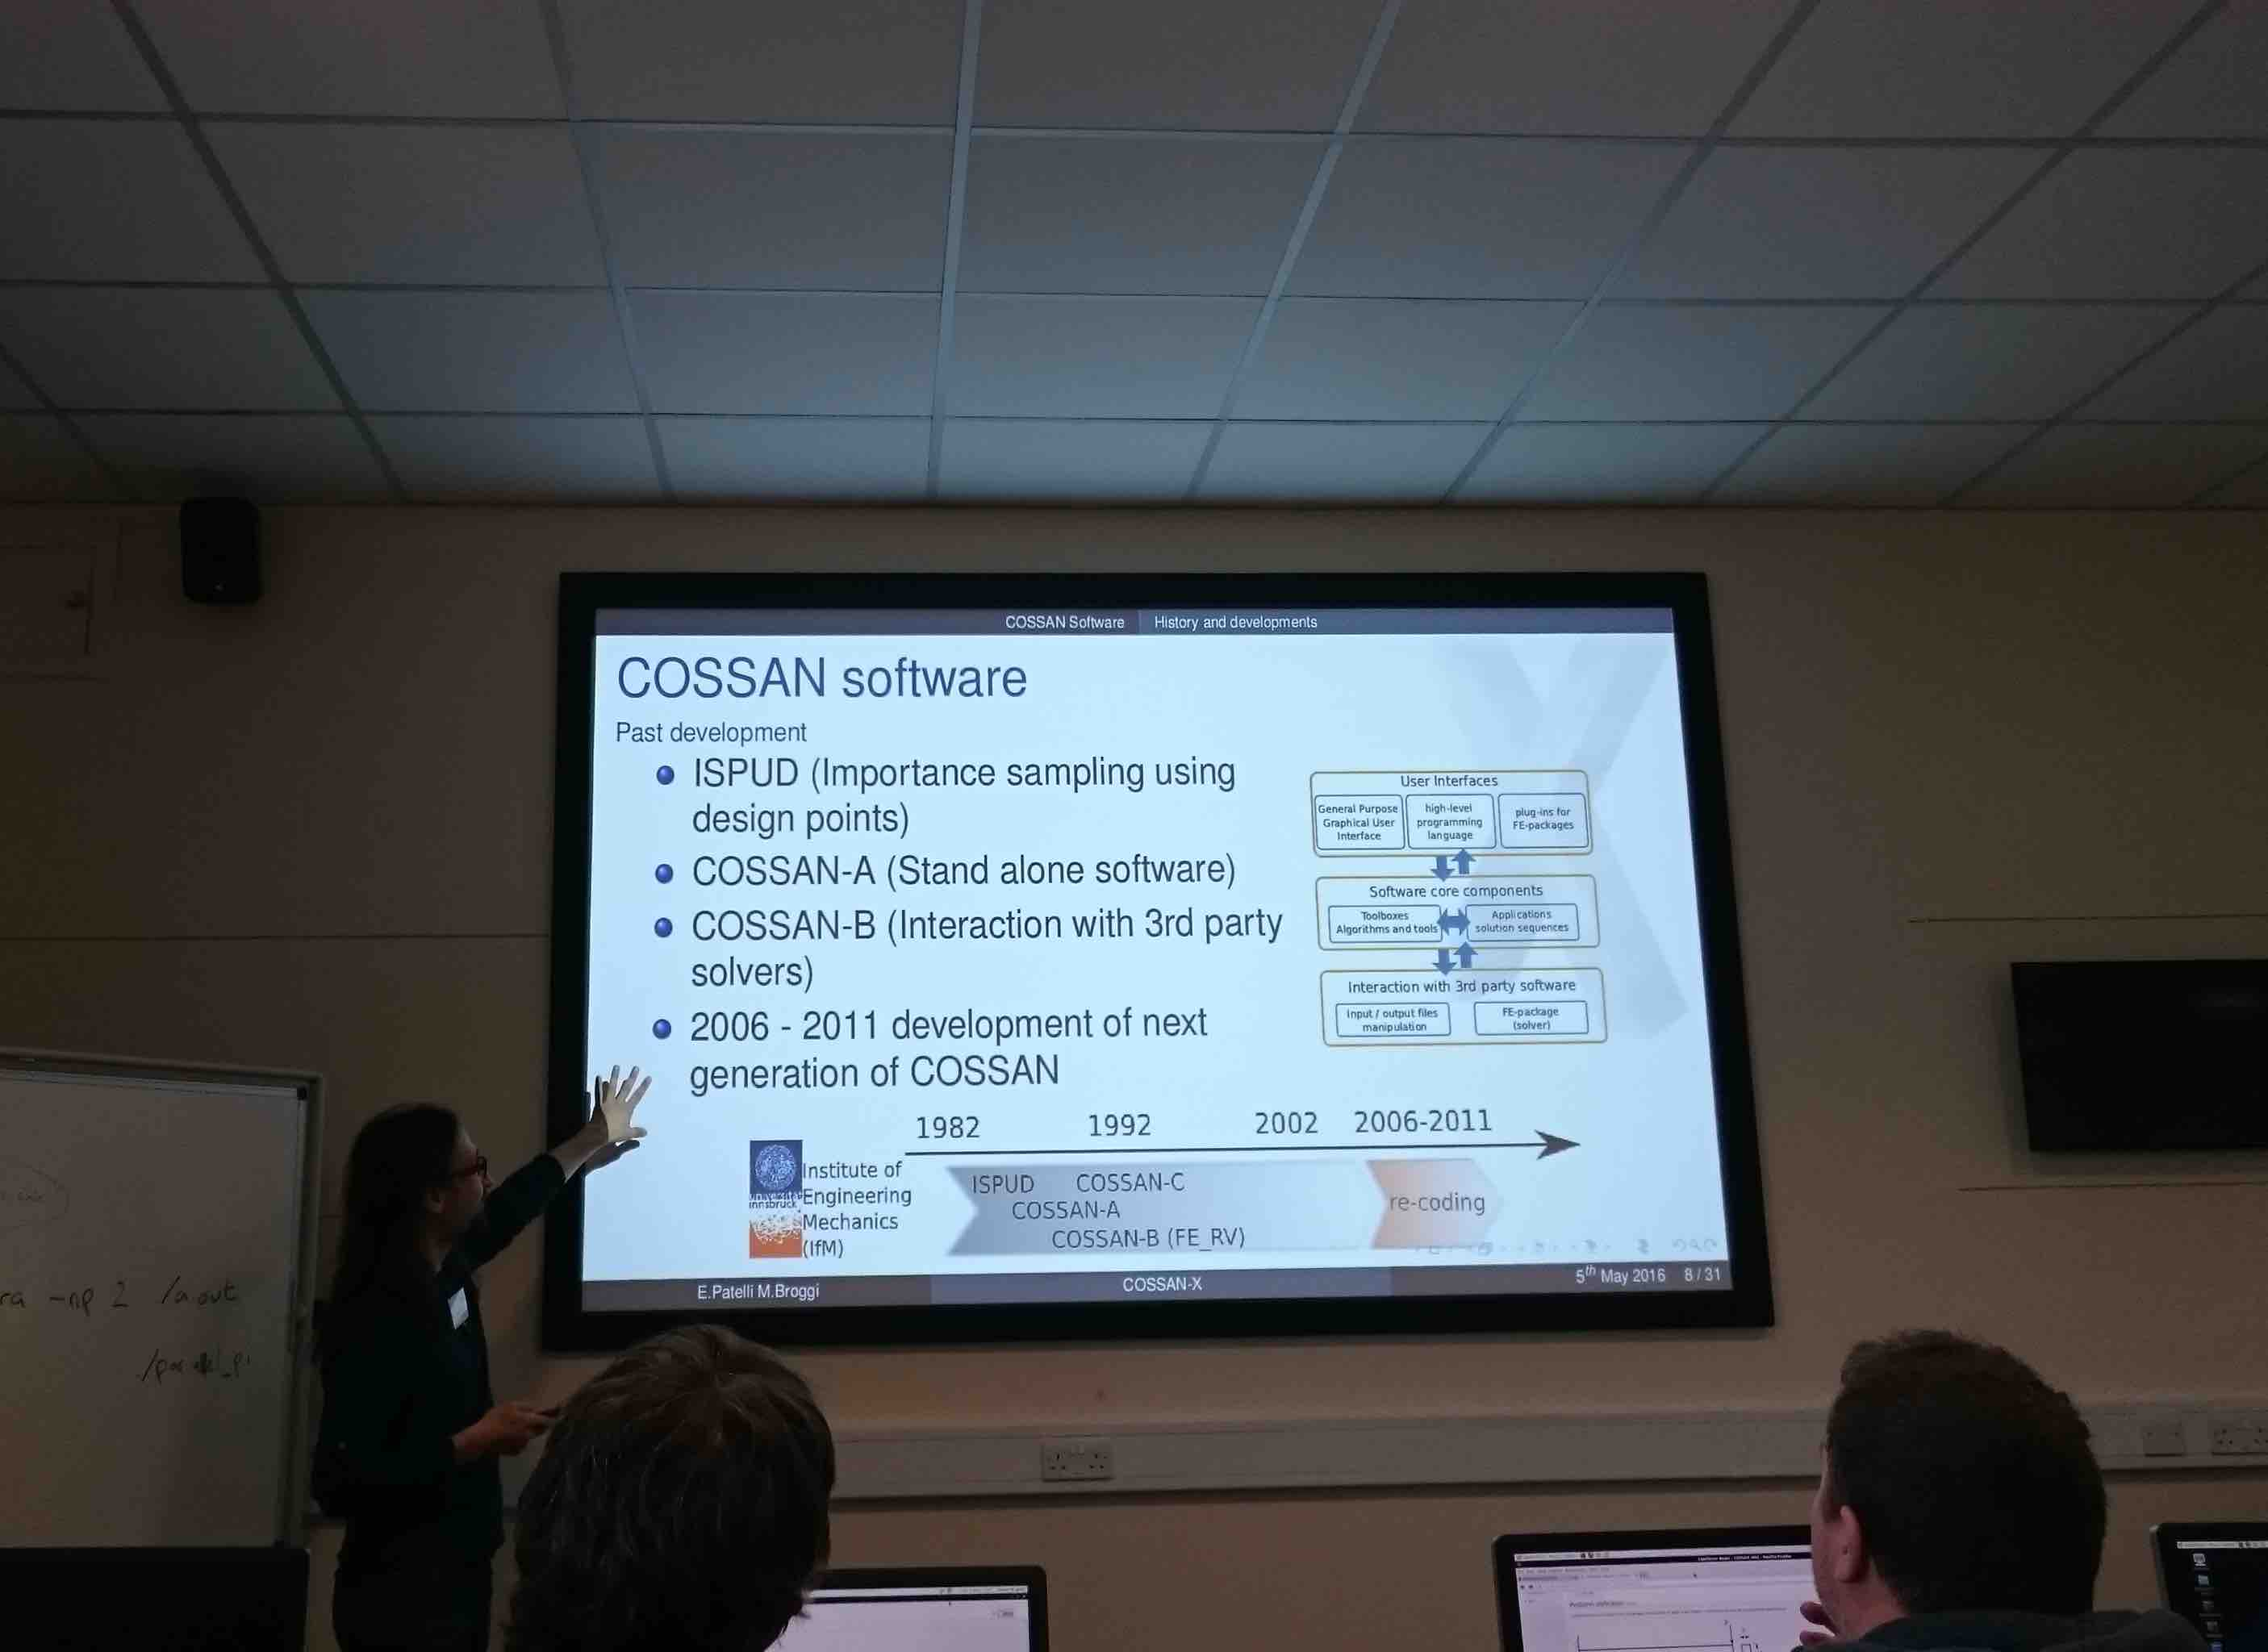
\includegraphics[width=0.95\linewidth]{training/edo1_lr.jpg}\\
{\small Dr Edoardo Patelli - University of Liverpool}
\end{center}
\end{minipage}
\begin{minipage}{0.6\textwidth}
{\bf Strucutre of the Training Programme}\\
Each day focuses on a specific topic. This allows the participation to attend a specific training day. The first day is dedicated to an introduction of general concepts of stochastic and probabilistic analysis as well as an introduction to High Performance Computing with practical exercises. The second day is dedicated to COSSAN-X software while the last day will concentrate on the OpenCossan software.

{\bf Aims and Learning outcomes}\\
The users have been taught the main techniques available for dealing with Risk and Uncertainty and how to use High Performance Computing to speed up the analysis.
\end{minipage}

For more information about the Course visit the webpage: \href{http://cossan.co.uk/training/training\_UQ2016.html#}{http://cossan.co.uk/training/training\_UQ2016.html}

















\cleardoublepage

\thispagestyle{Training}

\begin{minipage}{1.\textwidth}
\vspace{20pt}
{\LARGE {Cohort 2 visit the UoL's London Campus and Lloyd's Register}}\\ {\large 16$^{\text{th}}$ and 17$^{\text{th}}$ May 2016, London, UK}
\end{minipage}

\begin{minipage}{1.\textwidth}
\begin{figure}[H]
\centering
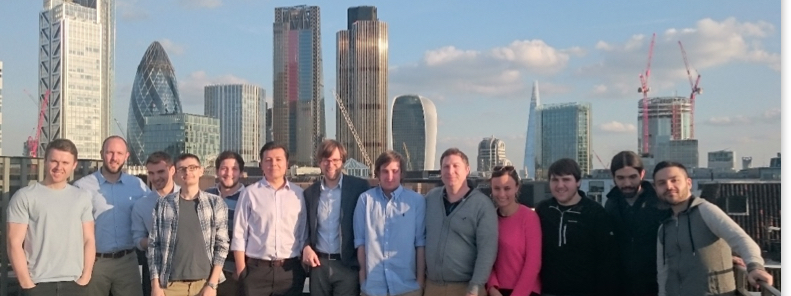
\includegraphics[width=0.9\linewidth]{training/LGroupPicture_2.jpg}\\
%{\small Group picture on the roof top of the UoL Building in Londond}
\end{figure}
\end{minipage}


%\vspace{10pt}

\begin{minipage}{1.\textwidth}
\begin{multicols}{2}
The Liverpool-based Centre for Doctoral Training (CDT) in Risk \& Uncertainty ran a two-day event, within the Masters of Research (MRes) training programme. Dr Alejandro Diaz, Programme Director of the MRes, and Dr Marco de Angelis, Manager of the CDT, accompanied the second cohort of CDT students to the University of Liverpool’s London Campus. The central location of the campus, in Finsbury Square, is an easy-access meeting point for companies and organisations based in and around the Capital.

The visit provided the Risk & Uncertainty CDT students with opportunities to engage with experts from a broad range of academic and industrial backgrounds. On this occasion, the students met Dr Kimmo Soram{\"a}ki, from Financial Network Analytics (FNA), who gave a lecture on Financial Cartography; namely the understanding of financial risk via correlation networks and other graphical tools.\\
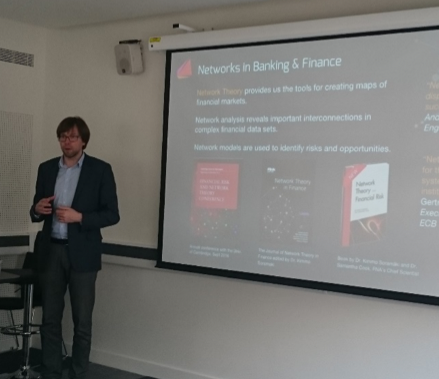
\includegraphics[width=0.48\linewidth]{training/Picture1.png}
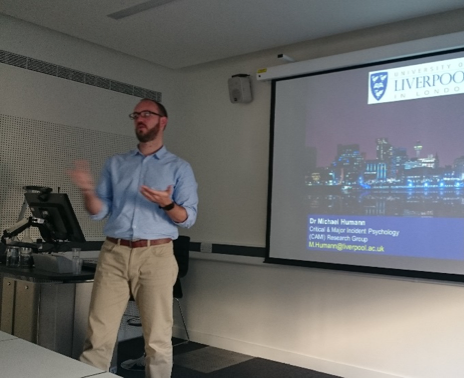
\includegraphics[width=0.51\linewidth]{training/Picture2.png}\\
{\footnotesize Dr Kimmo Soram{\"a}ki (FNA) and Dr Michael Humann (School of Psychology)}

Dr Michael Humann, from the School of Psychology, then gave a lecture on team work and risk communication, in preparation for the training exercise that the CDT students would have to go through later in the week. This was followed by a Q&A session with Dr Humann and Professor Laurence Alison (also from the School of Psychology) on public engagement and risk communication.

Day One finished with an informal networking forum, in the reception area of the London campus building. This was rounded-off by a stunning roof-top visit, which provided wonderful views over the city. 

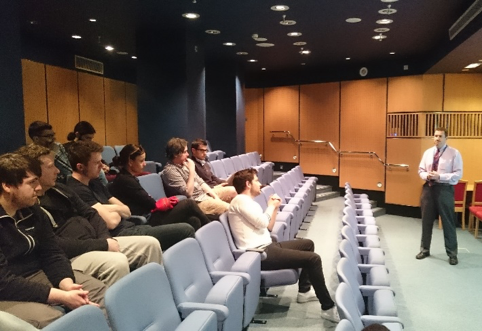
\includegraphics[width=0.5\linewidth]{training/Picture3.png}
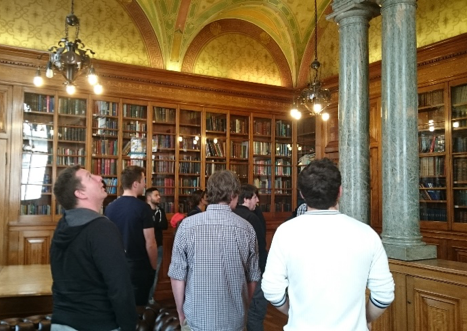
\includegraphics[width=0.485\linewidth]{training/Picture4.png}\\
{\footnotesize Lloyd's register theatre and historic library}

On Day Two of the London trip, Dr Diaz and Dr de Angelis went along with the CDT student group to visit Lloyd’s Register, whose roots in the city of London go back as far as 250 years. There, the students met experts and practitioners in transport classification and energy safety regulations. 

The visit was an exceptional opportunity for the students to acquire knowledge and understanding of risk from a more industry-focused perspective. It was also a chance for them to appreciate the history and evolution of standards and safety regulations. 
After the visit, the students returned to the University’s campus, where they participated in a 10kV test session developed by colleagues from the School of Psychology. This enabled the group to interact with each other and answer questions about decision-making and risk communication, as well as for them to provide feedback on the training module (RISK622) associated with the visit to London.\\
\BackToContents
\end{multicols}

\end{minipage}



















\cleardoublepage


\thispagestyle{Training}

\begin{minipage}{1.\textwidth}
\vspace{20pt}
{\LARGE {Risk Communication Workshop with National Nuclear Labs (NNL)}}\\
{\large 18$^{\text{th}}$ May 2016, Liverpool, UK}
\begin{multicols}{2}
The programme of the Master of Research in Decision Making under Risk and Uncertainty includes a core module called “Assessment and Communication of Risk”. The module examines quantitative tools, industrial experiences and psychological theories relating to the process of decision-making and communicating risk.

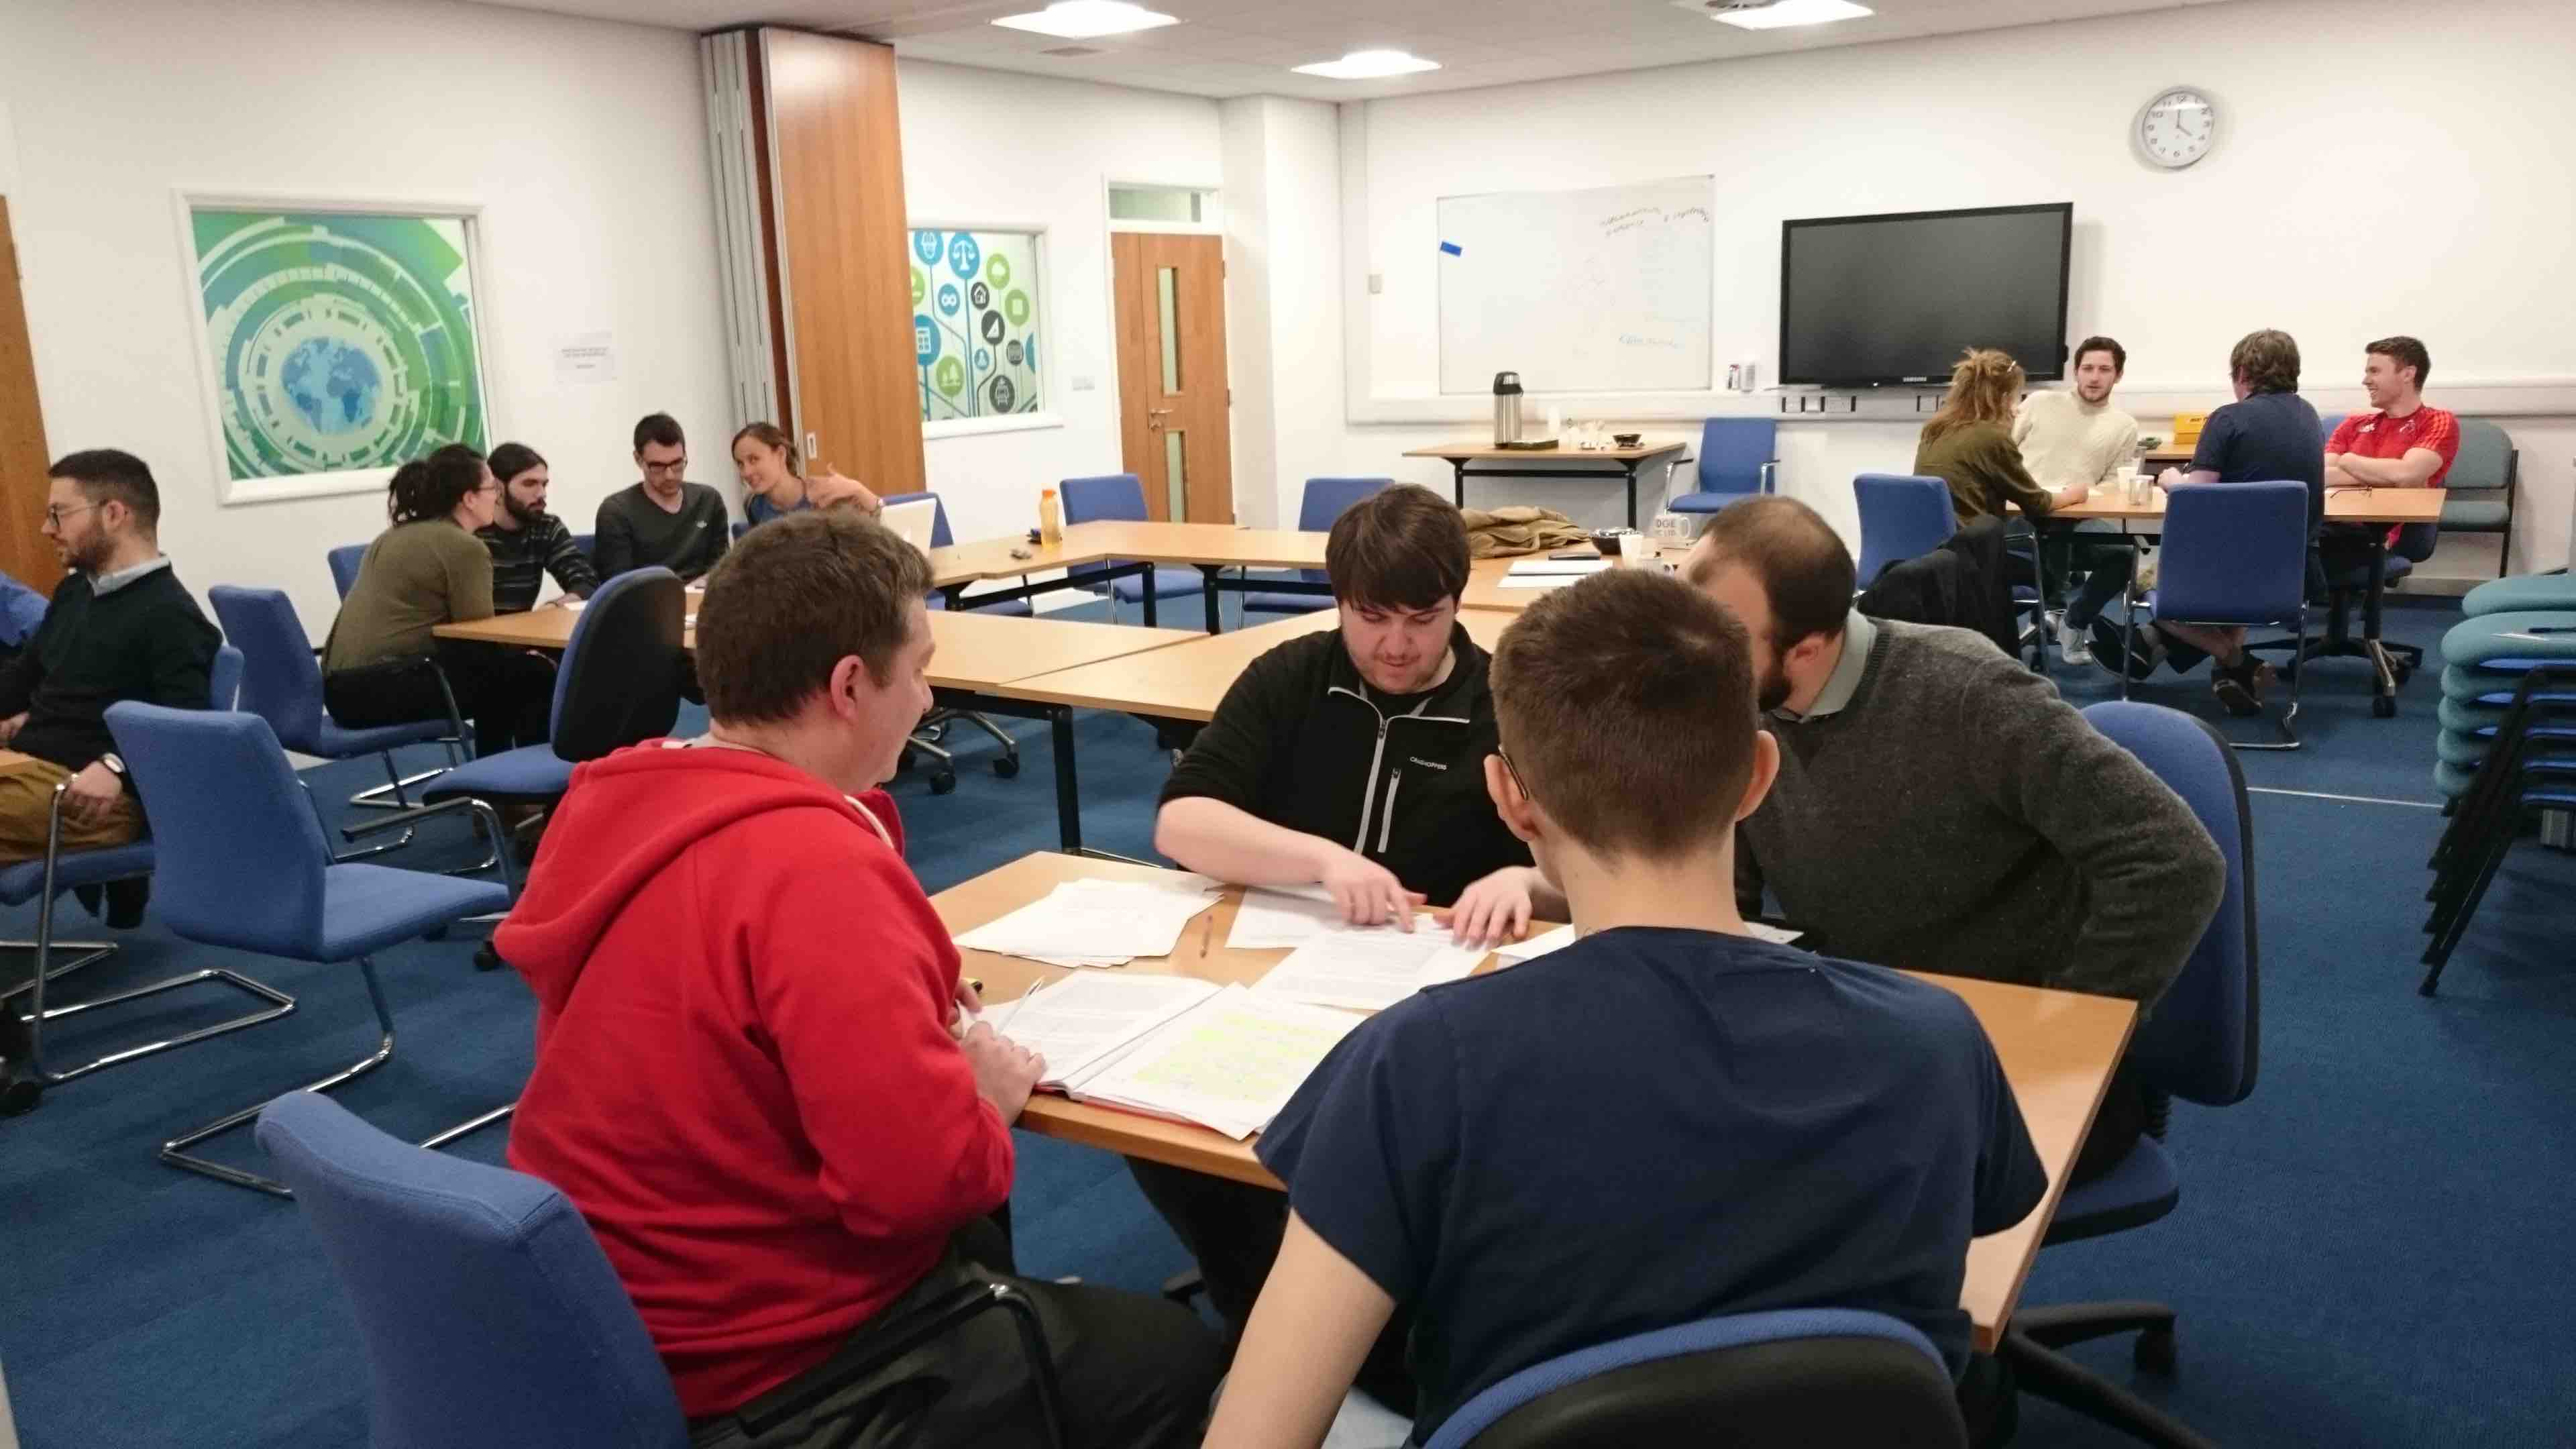
\includegraphics[width=1\linewidth]{training/Picture6.jpg}

This year one of the master classes was translated into a workshop to train the Master degree students to effectively communicate design decisions to a general audience of stakeholders. At the workshop a group of 4 experts from National Nuclear Laboratories (NNL) were invited to give a presentation and subsequently engage with the students in informal discussion groups.The students’ task was to solve an optimization problem and to try to find the best solution of deployment of a certain amount of radiation sensors to detect a radiation leak or any other potential nuclear threat cost efficiently; and subsequently communicate these findings via a press conference to the general public. 

The students had the opportunity to prepare beforehand for potential questions during the conference and ask NNL experts for their opinion and advice. They had to consider issues such as cost of a false alarm, the location of the sensors – the trip levels near nuclear power plants and elsewhere, the consequences of  missing a real “event”, at what point does the cost of sensors outweigh the potential benefit or the level of perception of potential threat by expert and by public. The task was not easy as the message had to be communicated clearly in a fairly short time frame and no jargon was to be used. 
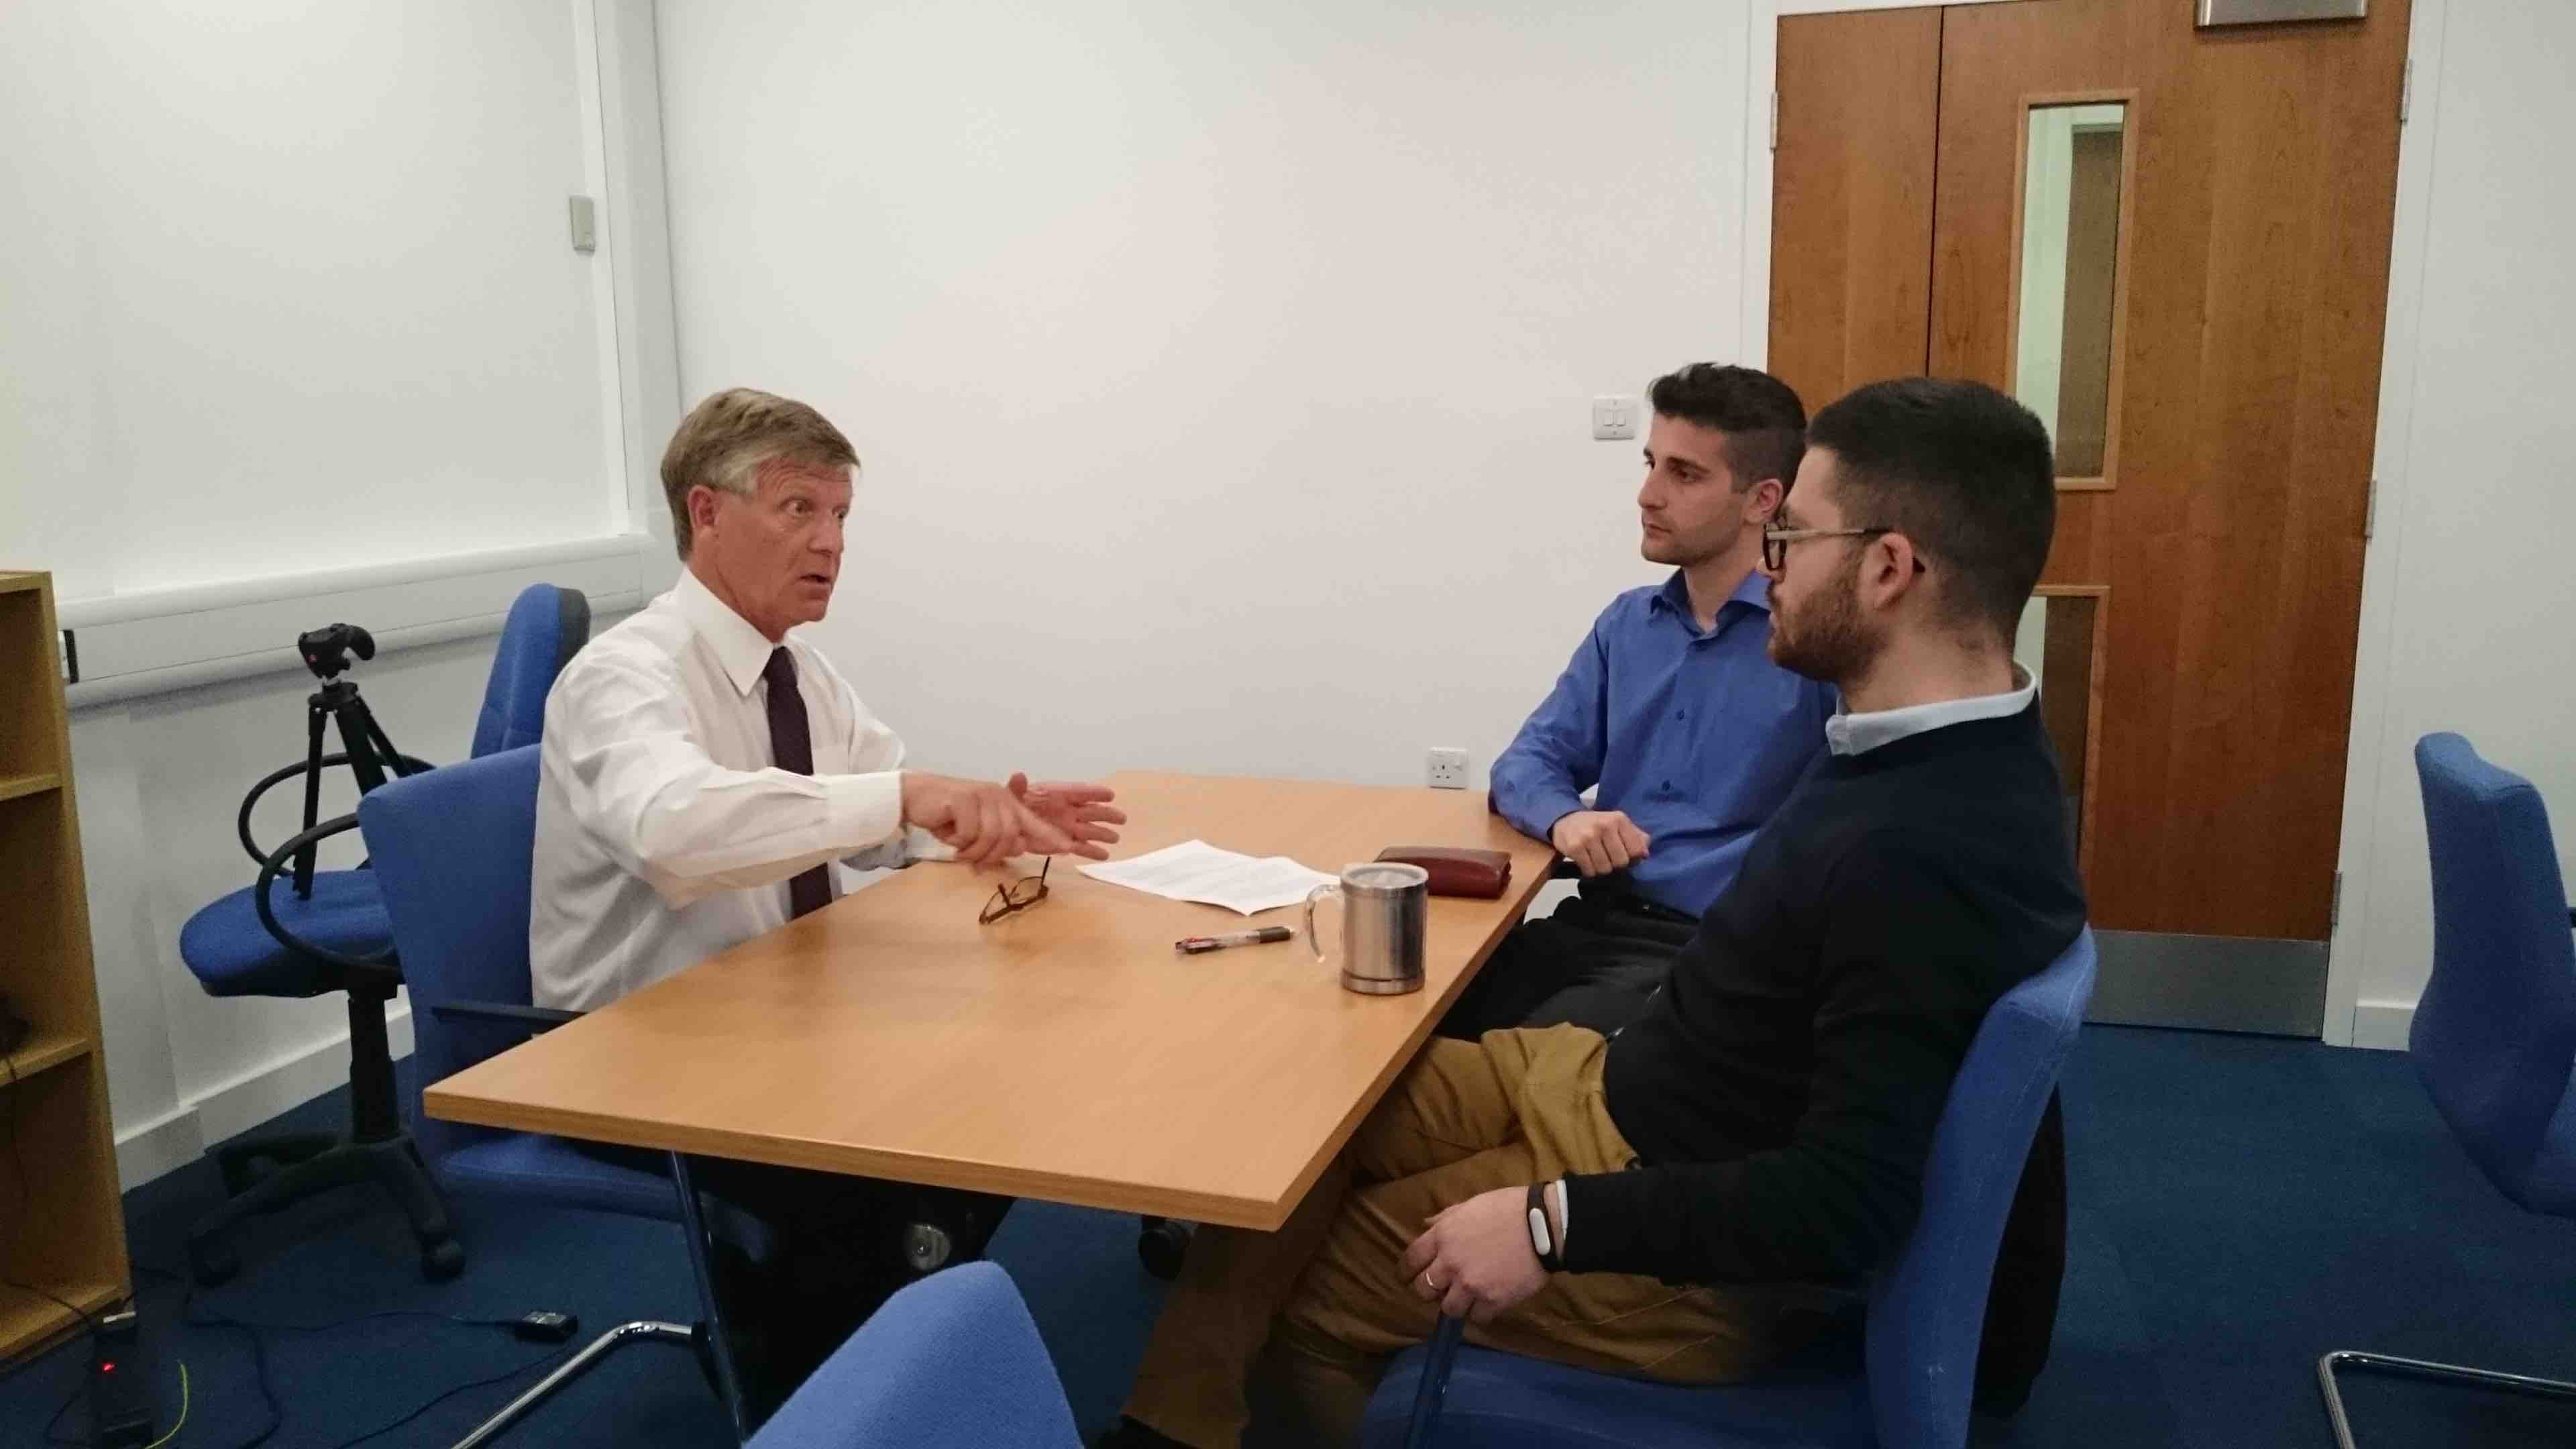
\includegraphics[width=1\linewidth]{training/Picture5.jpg}

\end{multicols}
\end{minipage}


%\begin{minipage}{1.\textwidth}
%\vspace{20pt}
%{\LARGE \href{https://www.liverpool.ac.uk/qfra/}{Summer School}, June 2016, Rhodes, Greece:}

%text
%\end{minipage}


\begin{minipage}{1.\textwidth}
\vspace{20pt}
{\LARGE {Poster Day at the Engineering Annual PhD Conference}}\\
{\large 1$^{\text{st}}$ July 2016, School of Engineering, University of Liverpool}

The Poster Day was organised within the MRes Programme as part of the RISK 661 module entitled ``Research Project''. Students had the opportunity to showcase their research to academics of the Risk Institute, to receive feedback and comments just a few months before they submit their research papers. The event was very well attended by staff members of the Risk Institute, which included as many as fifteen academics.

\begin{multicols}{2}

\includegraphics[width=1\linewidth]{training/Picture8.jpg}


\includegraphics[width=1\linewidth]{training/Picture7.jpg}

\end{multicols}
\end{minipage}



















\cleardoublepage

\thispagestyle{Training}
\begin{minipage}{1.\textwidth}
\vspace{20pt}
{\LARGE {2nd Symposium on Quantitative Finance and Risk Analysis (QFRA)}}\\
{\large 9$^{\text{th}}$ and 10$^{\text{th}}$ June 2016, Rhodes, Greece}
\begin{multicols}{2}
The multi-disciplinary Institute for Risk \& Uncertainty, through the EPSRC \& ESRC Centre for Doctoral Training on Quantification and Management of Risk and Uncertainty in Complex Systems & Environments and the Adam Smith Business School in the University of Glasgow organised the 2nd Symposium in Quantitative Finance and Risk Analysis (QFRA) in Rhodes, Greece from 9-10 June 2016.

\includegraphics[width=1\linewidth]{training/PictureSS1.png}

The symposium provided a multi-disciplinary forum for the exchange of knowledge and expertise in the broader area of Quantification Finance, Risk Analysis and Management. The event attracted 50 delegates from more than 10 countries, who are experts and decision makers in a variety of disciplines such as mathematics, economics, finance and engineering to name just a few. Invited speakers were:
\begin{itemize}
    \item Prof Bilal Ayyub, Centre for Technology and Systems Management, University of Maryland, USA. 
    \item Prof Michael Dempster, Centre for Financial Research, University of Cambridge, UK.
    \item Prof Marcel Prokopczuk, Institute for Financial Markets, Leibniz University Hannover, Germany
\end{itemize}
Two special issues have been dedicated to this event:
Journal of Commodity Markets (Elsevier) will publish a special conference issue on papers dedicated to ``Quantitative Analysis of Commodity Markets''. 
ASCE-ASME Journal of Risk and Uncertainty in Engineering Systems (ASCE publications) will publish a special conference issue on papers dedicated to “Community Resilience Economics”. 
For more details, please visit the \href{https://www.liverpool.ac.uk/qfra/}{QFRA2016 webpage}.

\includegraphics[width=1\linewidth]{training/QFRA2016_21.JPG}

\end{multicols}
\end{minipage}

\begin{minipage}{1.\textwidth}
\vspace{20pt}
{\LARGE {{\bf Upcoming ESRA Webinar}: \href{http://esra.eu-vri.eu/home.aspx?lan=230&tab=2768&itm=2768&pag=1082}{Alternative approaches to the treatment of epistemic uncertainties in risk assessment} - Prof Micheal Beer}}\\
{\large 2$^{\text{nd}}$ November 2016, 3.00 - 4.00 p.m. (GMT+1) }
\begin{multicols}{2}

Wednesday 2$^{\text{nd}}$ November 2016 from 3.00 to 4.00 p.m. (GMT+1), {\bf Prof Michael Beer}  will be teaching the ESRA Webinar: "Alternative approaches to the treatment of epistemic uncertainties in risk assessment". The webinar, Hosted by the European Safety and Reliability Association (ESRA),  will include a discussion on research opportunities in the international community. For more information about the speaker, to read the abstract and join the webinar go online here: \href{http://www.esrahomepage.eu}{http://www.esrahomepage.eu}

\end{multicols}
\end{minipage}




























\cleardoublepage

\thispagestyle{Training}
\begin{minipage}{1.\textwidth}
\vspace{20pt}
{\LARGE {Recent Trends in Decision Making under Risk and Uncertainty}}\\
{\large 19$^{\text{th}}$ September 2016, Shanghai, China}

\includegraphics[width=1\linewidth]{training/PictureThanasi2_crop.png}

The Institute for Risk & Uncertainty and the Management School in Shanghai University, China organized the {\bf International Workshop in Decision Making under Risk and Uncertainty} in Shanghai, China on 19 September 2016.
The event attracted more than 100 participants from 4 countries and 5 Chinese universities including Xi’an Jiaotong-Liverpool University.  

\begin{multicols}{2}


\includegraphics[width=1\linewidth]{training/PictureThanasi1_1.png}



\includegraphics[width=1\linewidth]{training/PictureThanasi1_2.png}

\end{multicols}
\end{minipage}






















\cleardoublepage

\thispagestyle{Symposia}

\begin{minipage}[t]{0.99\textwidth}
\hypertarget{Symposia}{\heading{Symposia in International Conferences}{6pt}}
\end{minipage}


\begin{minipage}[t]{0.15\textwidth}
\vspace{1pt}
\includegraphics[width=0.6\linewidth]{symposia/emi.jpeg}
\end{minipage}
\begin{minipage}[t]{0.79\textwidth}
\href{http://www.lem3.fr/2016EMI-IC/index.php?page=start}{EMI International Conference 2016},\\ 
25-27 Oct 2016, Metz, France\\
MS: Imprecise Recent Advances in Nonlinear Dynamics and Control: A Stochastic Perspective.\\
organised by M. Beer, I.A. Kougioumtzoglou, A.A. Pantelous, D. Yurchenko
\end{minipage}

\vspace{10pt}

\begin{minipage}[t]{0.15\textwidth}
\vspace{1pt}
\includegraphics[width=1\linewidth]{symposia/ieeeLogo.png}
\end{minipage}
\hspace{2pt}
\begin{minipage}[t]{0.79\textwidth}
IEEE Symposium Series on Computational Intelligence (SSCI)\\ 
Athens, Greece, December 6–9, 2016. \\
\href{http://ieeexplore.ieee.org/stamp/stamp.jsp?arnumber=7379091}{Symposium Computational Intelligence for Engineering Solutions (CIES)}\\ 
chaired by Prof Michael Beer, Prof Rudolf Kruse, Prof Vladik Kreinovich.
\end{minipage}

\vspace{10pt}

\begin{minipage}[t]{0.15\textwidth}
\vspace{1pt}
\includegraphics[width=1\linewidth]{symposia/ascelogo.png}
\end{minipage}
\hspace{2pt}
\begin{minipage}[t]{0.79\textwidth}
\href{}{ASCE Engineering Mechanics Institute Conference 2017},\\ 
4-7 Jun 2017, San Diego, USA\\
MS: Vibration measurement, modal analysis and model updating of structures.\\
chaired by Lam HF, Yang JH, Au SK
\end{minipage}

\vspace{10pt}

\begin{minipage}[t]{0.15\textwidth}
\vspace{1pt}
\includegraphics[width=1\linewidth]{symposia/uncecomp.png}
\end{minipage}
\hspace{2pt}
\begin{minipage}[t]{0.79\textwidth}
\href{https://2017.compdyn.org/}{2nd International Conference on Uncertainty Quantification in Computational Sciences and Engineering},\\ 
15-17 Jun 2017, Rhodes Island, Greece
\begin{itemize}
    \item[-] MS 2: ``Engineering Analyses with Vague and Imprecise Information'' (code MS-02-UB) organised by Edoardo Patelli (University of Liverpool, UK), Bruno Sudret (ETH Zurich, Switzerland), Matteo Broggi and Michael Beer (Leibniz University of Hannover, Germany)
    \item[-] MS 4: "Advanced simulation-based approaches to uncertainty quantification and reliability analysis" (code MS-04-UD) organised by Edoardo Patelli, Francisco Alejandro Diaz De la O (University of Liverpool, United Kingdom) and Siu-Kui Au (University of Liverpool, UK)
    \item[-] MS 6: ``Software for Uncertainty Quantification'' (code MS-06-UF) organised by Stefano Marelli, (ETH Zürich, Switzerland), Edoardo Patelli, Brian M. Adams (Sandia National Laboratories, United States) and Bruno Sudret.
\end{itemize}

\end{minipage}


\vspace{10pt}

\begin{minipage}[t]{0.15\textwidth}
\vspace{1pt}
\includegraphics[width=1\linewidth]{symposia/logo-icossar.png}
\end{minipage}
\hspace{2pt}
\begin{minipage}[t]{0.79\textwidth}
\href{http://www.icossar2017.org/}{12th International Conference on Structural Safety & Reliability (ICOSSAR 2017)}
\\ 
6-10 August, 2017. TU Wien Vienna, Austria.
\begin{itemize}
    \item[-] OS {\textit Uncertainty quantification for complex structures in dynamic environments.} Organized by Yurchenko/Beer/ Kougioumtzoglou/Chen/Li
    \item[-] MS {\textitImprecise probability methods in civil engineering.} Organized by Oberguggenberger/Beer/Patelli/Shields/Zhang 
    \item[-] MS {\textit Design of complex systems and structures under uncertain conditions.} Organized by Beck/Jensen/Beer/Valdebenito/Broggi
    \item[-] MS {\textitAdvances in simulation-based uncertainty quantification and reliability analysis.} Organised by Shields M, Au SK, Mahadevan S.
\end{itemize}
\end{minipage}


\vspace{10pt}

\begin{minipage}[t]{0.15\textwidth}
\vspace{1pt}
\includegraphics[width=1\linewidth]{symposia/eurodynLogo.png}
\end{minipage}
\hspace{2pt}
\begin{minipage}[t]{0.79\textwidth}
\href{http://eurodyn2017.it/}{10th International Conference on Structural Dynamics (EURODYN 2017)},\\ 
10-13 September 2017, Rome, Italy\\
MS: Reliability, robustness and design of complex and dynamical engineering systems.\\
chaired by Beck J, Jensen H, Au SK
\end{minipage}







%{\bf Keynote and Plenary Lectures:}

%\vspace{3pt}

%\begin{minipage}[t]{0.15\textwidth}
%%\includegraphics[width=1\linewidth]{symposia/logoISRERM.png}
%\end{minipage}
%\hspace{2pt}
%\begin{minipage}[t]{0.79\textwidth}
%2016, Aug 18: Keynote Lecture by Prof Michael Beer, 5th International Symposium on Reliability Engineering and Risk Management \href{http://www.isrerm2016.org/}{(ISRERM)} 
%\end{minipage}

%\vspace{3pt}

%\begin{minipage}[t]{0.15\textwidth}
%%\includegraphics[width=1\linewidth]{symposia/logoISRERM.png}
%\end{minipage}
%\hspace{2pt}
%\begin{minipage}[t]{0.79\textwidth}
%2016, Sept 14: Plenary Lecture by Prof Michael Beer, Colloquium on “Multi-uncertainty and Multi-scale Methods and related Applications” of the European Mechanics Society \href{www.euromech.org/conferences/EFMC/EFMC11}{(EUROMECH2016)} 
%\end{minipage}


%\vspace{10pt}




\cleardoublepage

\thispagestyle{Symposia}
\begin{minipage}{1.\textwidth}
\vspace{20pt}
{\LARGE {ASCE Workshop ``Resiliency of Urban Tunnels''}}\\
{\large 1$^{\text{st}}$ September 2016, ASCE Headqurters, VA, USA}

An international research consortia was formed to drive large scale developments in tunnel resilience and address needs with joint force. The ASCE Technical Report and follow up workshops will be held together with large grants applications. This workshop resulted as the collaboration between Tongji University, University of Maryland and Leibniz University Hannover.

\includegraphics[width=1\linewidth]{training/asceWorkshopFlyer.pdf}


\end{minipage}


















\cleardoublepage

\thispagestyle{Grants}

\begin{minipage}[t]{0.99\textwidth}
\vspace{5pt}
\hypertarget{Grants}{\Large{\bf Grants, Recognitions and Memberships}}
\end{minipage}

%{\bf Grants, Memberships and Recognitions:}

\begin{minipage}[t]{0.99\textwidth}
Congratulations to {\bf Prof Michael Beer} and {\bf Dr Edoardo Patelli} who won a grant within a Collaborative Research Center, titled: ``Risk Assessment of Regeneration Paths for Supporting Simultaneous Decisions'' by German Research Foundation, Grant No. D5 in SFB871, amount: E 126,600.

\vspace{10pt}

{\bf Prof Gabe Mythen} is President of the International Sociological Association Thematic Group the Sociology of Risk and Uncertainty
    (\href{http://www.isa-sociology.org/forum-2016/}{ISA conference} in Vienna).
    
\vspace{5pt}

{\bf Prof Ivan Au} is member of the scientific committee of the following international conferences:
    \begin{itemize}
        \item 10th International Conference on Structural Dynamics EURODYN 2017
        \vspace{5pt}
        \item 2nd International Conference on Uncertainty Quantification in Computational Sciences and Engineering
        \vspace{5pt}
        \item 7th International Workshop on Reliable Engineering Computing
        \vspace{5pt}
        \item 6th Asian-Pacific Symposium on Structural Reliability and its Applications
        \vspace{5pt}
        \item ASCE Engineering Mechanics Institute Conference 2016
    \end{itemize}
\vspace{5pt}
{\bf Prof Michael Beer} is member of the scientific committee of the following international conferences:
    \begin{itemize}
        \item 12th International Conference on Structural Safety and Reliability –  ICOSSAR2017
        \vspace{5pt}
        \item 3rd International Conference on Vulnerability and Risk Analysis and \& 7th International Symposium on Uncertainty Modelling and Analysis \& 4th International Symposium on Uncertainty Quantification and Stochastic Modeling – (ASCE-ICVRAM-ISUMA-UNCERTAINTIES 2018)
        \vspace{5pt}
        \item EMI (ASCE) International Conference 2016
        \vspace{5pt}
        \item  the 2nd International Conference on Uncertainty Quantification in Computational Sciences and Engineering – UNCECOMP 2017
        \vspace{5pt}
        \item Advisory Board and Technical Program Committee of the International Conference on Soft Computing in Engineering 2017
        \vspace{5pt}
        \item Program Committee of the International Conference on Information and Digital Technologies 2016 - IDT 2016
        \vspace{5pt}
        \item Scientific Committee of the 14th International Probabilistic Workshop - IPW 2016 
    \end{itemize}

{\bf Dr Edoardo Patelli} is Chair of the Technical Committee on Simulation for Safety and Reliability Analysis of European Safety and Reliability Association (ESRA), and is member of the scientific committee of the following international conferences:
    \begin{itemize}
        \item The annual European Safety and Reliability Conference (ESREL 2017)
        \vspace{5pt}
        \item Nuclear Power Plant Conference (NUPP 2017)
        \vspace{5pt}
        \item Conference on Parallel, Distributed, Grid and Cloud Computing for Engineering (PARENG 2017) 
    \end{itemize}


\vspace{5pt}    
{\Large{\bf Important Dates}}

The next {\bf Cossan Training Course} will be held at Tonjing University the {\bf 19th and 20th November 2016}. For more info: \href{http://cossan.co.uk/training/shanghai.php}{http://cossan.co.uk/training/shanghai.php}.

The next {\bf UQ\&M Study Group with Industry} will be held at the Institute for Risk \& Uncertainty, University of Liverpool, the {\bf 8th, 9th and 10th of March 2017}, contextually with the Stakeholder Workshop. For more info email Dr Marco De Angelis (marco.de-angelis@liverpool.ac.uk) or Dr Matt Butchers (KTN).

The next {\bf CDT Easter School} will be held at the Institute for Risk \& Uncertainty, University of Liverpool, the {\bf 19th, 20th and 21st of April 2017}. Registration will open in December 2016.

\end{minipage}















\cleardoublepage

\pagecolor{covercolor}\afterpage{\nopagecolor}

\thispagestyle{Projects}

\begin{minipage}[t]{0.99\textwidth}
\hypertarget{Projects}{\heading{Cohort 3: Student Projects starting in October 2016}{6pt}}
\end{minipage}

%The studentships are granted for 4 years and include, in the first year, a Master in Decision Making under Risk \& Uncertainty. The projects include extensive collaboration with prime industry to build an optimal basis for employability.

%The projects will commence October 2016.
\vspace{5pt}
%{\small Please apply online to the \emph{School of Engineering} providing the title and the name of the primary supervisor.}

\begin{minipage}{0.99\textwidth}

\begin{itemize}
{\small
\item {\bf Addressing the Risk of Food Security and Antimicrobial Resistance via Advanced Monitoring Techniques};
%{\footnotesize
\textit{Student}: Jodie Barber (Microbiology). 
\textit{Supervisors}: Prof Rasmita Raval (50{\%}), Chemistry; Dr Daimark Bennett (25{\%}), Integrative Biology; Heather Allison (25{\%}) Biological Sciences;\\
\textit{Industry Partner}: Croda 
%}
\vspace{5pt}
\item {\bf Stigmergy-based mapping of indoor hazardous environments};
\textit{Student}: James Butterworth (Computer Science). 
\textit{Supervisors}: Prof Karl Tuyls (60{\%}), Computer Science; Dr Paolo Paoletti (40{\%}), Engineering; \\
\textit{Industry Partner}: National Nuclear Laboratory
\vspace{5pt}
\item {\bf Living and Future Tools for Risk Assessment: An Examination of the Possibilities for Fusion};
\textit{Student}: Atousa Khodadadyan (Risk Management). 
\textit{Supervisors}: Professor Gabe Mythen (50{\%}), Sociology; Dr Hirbod Assa (30{\%}), Mathematical Sciences; Beverley Bishop (20{\%}), Health \& Safety Executive; \\
\textit{Industry Partner}: Health \& Safety Executive
\vspace{5pt}
\item {\bf Neural mechanisms of effort-based decision making};
\textit{Student}: Adam Byrne (Psychology). 
\textit{Supervisors}: Dr Andrej Stancak (60{\%}), Psychological Sciences, Dr Athanasios Pantelous (40{\%}), Mathematical Sciences; \\
\textit{Industry Partner}: Unilever
\vspace{5pt}
\item {\bf Rapid Screening Mass Spectrometry for Detection of Marine Toxins in Aquatic Food};
\textit{Student}: Barry Smith (Electrical Engineering).  
\textit{Supervisors}: Dr Simon Maher (70{\%}), Electrical Engineering \& Electronics; Dr Iain Young (30{\%}), Integrative Biology; \\
\textit{Industry Partner}: Q-Technologies
\vspace{5pt}
\item {\bf Training \& Learning Evaluation Frameworks: Monitoring Skills \& Knowledge Audits};
\textit{Student}: Darren Cook (Psychology).  
\textit{Supervisors}: Professor Laurence Alison (35{\%}), Psychology; Professor Simon Maskell (35{\%}), Electrical Engineering; Dr Michael Humann (30{\%}), Psychology; \\
\textit{Industry Partner}: National Counter Terrorism Unit, London Fire Brigade, Merseyside Fire \& Rescue
\vspace{5pt}
\item {\bf Big Data Adaptive Dynamic Route Planning for High-Sea Transportations};
\textit{Student}: No{\'e}mie Le Carrer (Physics). 
\textit{Supervisors}: Dr Jeyan Thiyagalingam (80{\%}), Electrical Engineering \& Electronics; Dr Peter Green (20{\%}), Engineering; \\
\textit{Industry Partner}: Hartree - STFC, Lloyds Register
\vspace{5pt}
\item {\bf Automatic Balancing Mechanisms in Public Pension Systems: A Solution to Face Demographic and
 Economic Risks?}
\textit{Student}: Maria Ferrer Fernandez (Mathematics). 
\textit{Supervisors}: Dr Carmen Boado Penas (70{\%}), Mathematical Sciences; Professor Brendan McCabe (30{\%}), Management School; \\
\textit{Industry Partner}: Swedish Pension Agency
\vspace{5pt}
\item {\bf Farming in transition in East Africa: financial risk taking and agricultural intensification};
\textit{Student}: Eleanor Balchin (International Development). 
\textit{Supervisors}: Professor Eric F{\'e}vre (50{\%}), Dr Rob Christley (10{\%}), Institute of Infection \& Global Health; Professor Jude Robinson (40{\%}), Sociology; \\
\textit{Industry Partner}: Financial Sector Development Programme
\vspace{5pt}
\item {\bf Testing the robustness of base-lined data required to assess and mitigate flood risk in 
lacustrine environments using multi-proxy evidence};
\textit{Student}: Hazel Phillips (Engineering). 
\textit{Supervisors}: Dr Neil Macdonald (40{\%}), Physical Geography; Professor Richard Chiverrell (40{\%}), Physical Geography, Dr Jonathan Bridge (20{\%}), Environmental Engineering, School of Engineering; \\
\textit{Industry Partner}: Environment Agency, NERC
}
\end{itemize}

%\begin{multicols}{2}
%\begin{footnotesize}
%%\begin{itemize}
%\begin{enumerate}
%	\item \href{https://www.liverpool.ac.uk/risk-and-uncertainty/postgraduate/cdt-research-projects-available/interbank-systems/}{Circular Layouts Representation of the Interbank Systems}(Mathematical Sciences / Engineering);
%	\item \href{https://www.liverpool.ac.uk/risk-and-uncertainty/postgraduate/cdt-research-projects-available/neural-mechanisms-of-effort-based-decision-making}{Neural mechanisms of effort-based decision making} (Psychological Sciences / Mathematical Sciences);
%	\item \href{https://www.liverpool.ac.uk/risk-and-uncertainty/postgraduate/cdt-research-projects-available/design-decision-tool/}{Development of a Robust Client Interface Design Decision Tool} (Engineering / Architecture);
%	\item \href{https://www.liverpool.ac.uk/risk-and-uncertainty/postgraduate/cdt-research-projects-available/structural-restoration-and-refurbishment}{Development of Sensible Structural Restoration and Refurbishment Analysis Methods} (Engineering / Architecture);	
%	\item \href{https://www.liverpool.ac.uk/risk-and-uncertainty/postgraduate/cdt-research-projects-available/risk-robust-analysis}{Reliability/Robustness-Based Approaches and Computational Tools for Multidisciplinary Systems under Mixed Aleatory and Epistemic Uncertainty} (Engineering / Environmental Sciences);
%	\item \href{https://www.liverpool.ac.uk/risk-and-uncertainty/postgraduate/cdt-research-projects-available/software-stochastic-analysis-large-scale-systems}{Efficient and Energy-Aware Software for Stochastic Analysis on Large-Scale Systems} (Engineering / Computer Science);
%	\item \href{https://www.liverpool.ac.uk/risk-and-uncertainty/postgraduate/cdt-research-projects-available/reinforced-concrete-near-field-explosions}{Reinforced Concrete Response to Near Field Explosions} (Civil / Structural Engineering);
%	\item \href{https://www.liverpool.ac.uk/risk-and-uncertainty/postgraduate/cdt-research-projects-available/stigmergy-based-mapping-indoor-hazardous-environments}{Stigmergy-based mapping of indoor hazardous environments}(Computer Science / Engineering);
%	\item \href{https://www.liverpool.ac.uk/risk-and-uncertainty/postgraduate/cdt-research-projects-available/electric-freight-vehicle/}{Quantification and management of the uncertainties of electric freight vehicle and failure modes analysis of aluminium foam structures} (Engineering / Computer Science);
%	\item \href{https://www.liverpool.ac.uk/risk-and-uncertainty/postgraduate/cdt-research-projects-available/modelling-measuring-risk-ict/}{Modeling and measuring risk in the Context of the Business Use of Information and Communication Technology (ICT)} (Management School / Mathematical Sciences);
%	\item \href{https://www.liverpool.ac.uk/risk-and-uncertainty/postgraduate/cdt-research-projects-available/risk-communication-major-incidents}{Improving multi-agency risk communication in major incidents}  (Psychology / Electrical Engineering);
%	\item \href{https://www.liverpool.ac.uk/risk-and-uncertainty/postgraduate/cdt-research-projects-available/balancing-critical-decisions}{Balancing ethicalilty, legality, security and safety critical decisions}  (Computer Science / Psychology);
%	\item \href{https://www.liverpool.ac.uk/risk-and-uncertainty/postgraduate/cdt-research-projects-available/fingerprinting-sources-of-sediment/}{Fingerprinting sources of sediment pollution in agricultural river systems} (Engineering / Environmental Sciences);
%	\item \href{https://www.liverpool.ac.uk/risk-and-uncertainty/postgraduate/cdt-research-projects-available/training-learning-evaluation-frameworks/}{Training \& Learning Evaluation Frameworks: Monitoring Skills \& Knowledge Audits} (Psychology / Computer Science);
%	\item \href{https://www.liverpool.ac.uk/risk-and-uncertainty/postgraduate/cdt-research-projects-available/estimating-energy-efficiency/}{Estimating Energy Efficiency of Applications on HPC Resources} (Electrical Engineering, Electronics and Computer Science / Engineering);
%	\item \href{https://www.liverpool.ac.uk/risk-and-uncertainty/postgraduate/cdt-research-projects-available/socio-ecological-networks/}{Untangling Risk and Uncertainty in Socio-ecological Networks} (Environmental Sciences / Engineering)
%	\item \href{https://www.liverpool.ac.uk/risk-and-uncertainty/postgraduate/cdt-research-projects-available/high-sea-transportations/}{Big Data Adaptive Dynamic Route Planning for High-Sea Transportations}  (Electrical Engineering, Electronics and Computer Science / Engineering);
%	\item \href{https://www.liverpool.ac.uk/risk-and-uncertainty/postgraduate/cdt-research-projects-available/hormone-analysis-aquaculture/}{Hormone Analysis in Aquaculture and Laboratory Fish Culture} (Electrical Engineering and Electronics / Institute of Integrative Biology);
%	\item \href{https://www.liverpool.ac.uk/risk-and-uncertainty/postgraduate/cdt-research-projects-available/marine-toxins-aquatic-food-sources/}{Rapid Screening Mass Spectrometry for Detection of Marine Toxins in Aquatic Food Sources} (Electrical Engineering and Electronics / Institute of Integrative Biology);
%	\item \href{https://www.liverpool.ac.uk/risk-and-uncertainty/postgraduate/cdt-research-projects-available/drought-risk/}{Drought Risk} (Environmental Sciences / Engineering);
%	\item \href{https://www.liverpool.ac.uk/risk-and-uncertainty/postgraduate/cdt-research-projects-available/flood-risk-lacustrine-environments}{Testing the Robustness of the Base-Line Data Required to Assess and Mitigate Flood Risk in Lacustrine Environments Using Multi-Proxy Evidence} (Environmental Sciences / Engineering);
%	\item \href{https://www.liverpool.ac.uk/risk-and-uncertainty/postgraduate/cdt-research-projects-available/in-situ-speciation-trace-metals}{In-situ Speciation of Trace Metals in Marine Systems} (Environmental Sciences / Institute of Integrative Biology);
%	\item \href{https://www.liverpool.ac.uk/risk-and-uncertainty/postgraduate/cdt-research-projects-available/uncertainties-flood-risk-modelling/}{Uncertainties in Flood Risk Modelling: Effect of Changing River Morphology on Flow Resistance} (Environmental Sciences / Engineering)
%	\item \href{https://www.liverpool.ac.uk/risk-and-uncertainty/postgraduate/cdt-research-projects-available/predicitive-modelling-interbank-markets/}{Predictive Modelling for Interbank Markets} (Computer Science - Autonomous Systems and Robotics / Economics and Computation);
%	\item \href{https://www.liverpool.ac.uk/risk-and-uncertainty/postgraduate/cdt-research-projects-available/coastal-erosion-flooding-management/}{Risk and Uncertainties in Applying Process Based Morphological Model to Offshore Wind Farm Induced Coastal Erosion and Flooding Management} (Engineering / Environmental Sciences)
%	\item \href{https://www.liverpool.ac.uk/risk-and-uncertainty/postgraduate/cdt-research-projects-available/scour-offshore-wind-farm-foundations/}{Risk and uncertainties in prediction of scour around offshore wind farm foundations} (Engineering / Environmental Sciences)
%	\item \href{https://www.liverpool.ac.uk/risk-and-uncertainty/postgraduate/cdt-research-projects-available/charged-particles-mass-spectrometry/}{Deposition of Charged Particles via Preparative Mass Spectrometry} (Electrical Engineering \& Electronics / Engineering);
%	\item \href{https://www.liverpool.ac.uk/risk-and-uncertainty/postgraduate/cdt-research-projects-available/fatigue-risk-management/}{Fatigue Risk Management in the Workplace}(Electrical Engineering \& Electronics / Psychology / Engineering);
%	\item \href{https://www.liverpool.ac.uk/risk-and-uncertainty/postgraduate/cdt-research-projects-available/farming-east-africa/}{Farming in transition in East Africa: financial risk taking and agricultural intensification} (Infection \& Global Health / Sociology)
%	\item \href{https://www.liverpool.ac.uk/risk-and-uncertainty/postgraduate/cdt-research-projects-available/food-resilience-aquaponics/}{Food Resilience by Aquaponics} (Integrative Biology / Computer Science);
%	\item \href{https://www.liverpool.ac.uk/risk-and-uncertainty/postgraduate/cdt-research-projects-available/living-and-future-tools/}{Living and Future Tools for Risk Assessment: An Examination of the Possibilities for Fusion} (Sociology / Mathematical Sciences);
%	\item \href{https://www.liverpool.ac.uk/risk-and-uncertainty/postgraduate/cdt-research-projects-available/social-security-orphans-widows/}{European Pensions Systems for Survivors (Orphans and Widows)}  (Mathematical Sciences / Sociology).
%\end{enumerate}
%%\end{itemize}
%\end{footnotesize}
%\end{multicols}
\end{minipage}

\vspace{10pt}

{\large \bf Acknowledgements}:\\
The Engineering \& Physical Science Research Council (\href{https://www.epsrc.ac.uk}{EPSRC}) and the Economic \& Social Research Council (\href{www.esrc.ac.uk}{ESRC}) are greatly acknowledged for their funding and support to the Centre for Doctoral Training in Quantification of Risk and Uncertainty in Complex Systems and Environments.\\
\href{https://www.epsrc.ac.uk}{\includegraphics[width=0.23\textwidth]{logos/EPSRC.png}}
\href{www.esrc.ac.uk}{\includegraphics[width=0.12\textwidth]{logos/Esrc_logo.png}}
\hspace{10pt}
\href{https://www.liverpool.ac.uk/}{\includegraphics[width=0.4\textwidth]{logos/university.png}}\\
\BackToContents
\end{document} 

